% =============================================================================
%  MEng Final Year Project Report
%  Safety-Aware Reinforcement Learning for ISO 15066-Compliant
%  Humanoid Manipulation Under Sustained Co-Working
%
%  Author: Ayush Patel
%  Department of Computing, Imperial College London
%
%  PAGE LIMIT: 60 A4 pages of content (everything between the contents
%  page and the reference list, exclusive). This is a limit, not a target.
%
%  v16 (2026-06-11): clarity reframe. One thesis (the regime map), three
%  RQs mapped 1:1 onto three results movements, five contributions.
%  Experiment codes (E n.m / R0-R3 / C1-C6 / Phase n) removed from prose
%  and headings; stated once parenthetically per experiment and indexed
%  in Appendix "Experiment Code Index". v15 backup: main_v15_backup.tex;
%  change log: CHANGELOG_v16.md (v13 history: CHANGELOG_v13.md).
%
%  STRUCTURE (8 content chapters):
%    Ch. 1 Introduction  (thesis box + regime-map schematic, 3 RQs, 5 contribs)
%    Ch. 2 Background and Related Work
%    Ch. 3 The safety_bigym Benchmark  (env + metrics + co-working + demos)
%    Ch. 4 Methods: The Two Parts of the Hybrid Safety Critic
%    Ch. 5 Measuring Safety Beside a Person  (tasks, axes, protocol, baselines)
%    Ch. 6 Results: Two Regimes, One Boundary  (persistent -> intermittent -> boundary)
%    Ch. 7 Discussion
%    Ch. 8 Conclusions and Future Work
%
%  CITATIONS: Vancouver style via natbib + vancouver.bst.
%
%  Draft markers (\placeholder / \result / \todo) are defined below for
%  editing convenience; the submitted text contains none.
%
%  Compile:
%    pdflatex report && bibtex report && pdflatex report && pdflatex report
% =============================================================================

\documentclass[11pt,a4paper]{report}

% === Packages ===
\usepackage[utf8]{inputenc}
\usepackage[T1]{fontenc}
\usepackage{lmodern}
\usepackage[british]{babel}
\usepackage{microtype}
\setlength{\emergencystretch}{3em} % relieve minor overfull lines from long \texttt{} identifiers
\usepackage{geometry}
  \geometry{a4paper, margin=2.5cm}
\usepackage{graphicx}
\usepackage{booktabs}
\usepackage{array}     % >{\raggedright\arraybackslash}p{} wrapping columns
\usepackage{multirow}
\usepackage{amsmath, amssymb, amsthm}
\usepackage{mathtools}
% algorithm float via float.sty shim (algorithm.sty absent from the local
% TeX Live; behaviour identical for this document's single algorithm)
\usepackage{float}
\newfloat{algorithm}{htbp}{loa}[chapter]
\floatname{algorithm}{Algorithm}
\usepackage{algpseudocode}
\usepackage{xcolor}
\usepackage{enumitem}
\usepackage{tikz}
  \usetikzlibrary{positioning, arrows.meta, fit, backgrounds, shapes.geometric, calc}
\usepackage{pgfplots}
  \pgfplotsset{compat=1.18}
  % NOTE: results plots (E3.2, E4.3, E5.2) below use pgfplots with
  % PLACEHOLDER coordinates. Replace the marked data with measured
  % values, or drop in a matplotlib-exported PDF instead.
% compact heading spacing (page budget; 11pt body text untouched)
\usepackage{titlesec}
\titleformat{\chapter}[hang]{\huge\bfseries}{\thechapter\quad}{0pt}{\huge\bfseries}
\titlespacing*{\chapter}{0pt}{0pt}{18pt}
\titlespacing*{\section}{0pt}{10pt plus 2pt minus 2pt}{5pt plus 1pt}
\titlespacing*{\subsection}{0pt}{8pt plus 2pt minus 2pt}{4pt plus 1pt}
\usepackage{caption}
  \captionsetup{font=small, skip=5pt}
\usepackage{subcaption}
% tighter float spacing (page-budget; standard 11pt text leading unchanged)
\setlength{\floatsep}{8pt plus 2pt minus 2pt}
\setlength{\textfloatsep}{10pt plus 2pt minus 4pt}
\setlength{\intextsep}{8pt plus 2pt minus 2pt}
% discourage sparse float pages: floats must share pages with text unless
% the float page is ≥85% full
\renewcommand{\topfraction}{0.92}
\renewcommand{\bottomfraction}{0.6}
\renewcommand{\textfraction}{0.06}
\renewcommand{\floatpagefraction}{0.85}
\usepackage{pifont}   % checkmarks, ding glyphs for benchmark comparison table

% === Vancouver-style numerical citations ===
% natbib with numbers+square+sort&compress gives [1], [2,3], [1-3].
% vancouver.bst renders the bibliography in Vancouver style.
\usepackage[numbers, sort&compress, square]{natbib}
\setcitestyle{numbers}
\bibliographystyle{vancouver}

\usepackage{hyperref}
  \hypersetup{colorlinks=true, linkcolor=black, citecolor=blue, urlcolor=blue}
\usepackage{cleveref}

% === Theorem environments ===
\newtheorem{theorem}{Theorem}[chapter]
\newtheorem{proposition}[theorem]{Proposition}
\newtheorem{lemma}[theorem]{Lemma}
\newtheorem{corollary}[theorem]{Corollary}

% === Convenience macros ===
\newcommand{\ssm}{SSM}
\newcommand{\pfl}{PFL}
\newcommand{\iso}{ISO~15066}
\newcommand{\cvar}{\ensuremath{\mathrm{CVaR}}}
\newcommand{\bigym}{\textsc{BiGym}}
\newcommand{\sbigym}{\texttt{safety\_bigym}}
\newcommand{\cqnas}{CQN-AS}
\newcommand{\coworker}{\textsc{coworker}}
\newcommand{\bodyslampp}{BodySLAM\nolinebreak[4]\hspace{-.05em}\raisebox{.2ex}{\scriptsize ++}}
\newcommand{\todo}[1]{\textcolor{red}{\textbf{TODO:} #1}}
\newcommand{\placeholder}[1]{\textcolor{gray!75!black}{\textit{[#1]}}}
\newcommand{\result}[1]{\textbf{[\textit{#1}]}}
\newcommand{\cmark}{\ding{51}}
\newcommand{\xmark}{\ding{55}}

\title{\sbigym{}: A Benchmark and a Co-location Regime Map\\
       for Safe Humanoid Manipulation\\
       Alongside a Live Human Coworker}
\author{Ayush Patel \\
        Department of Computing \\
        Imperial College London \\[1ex]
        Supervisor: Stephen James}
\date{June 2026}

% =============================================================================
\begin{document}
% =============================================================================
\maketitle

% ===
\begin{abstract}
\noindent
Learned humanoid manipulators can now work in the same space a person
reaches into. Their policies, however, are usually trained to optimise
task reward. They do not directly optimise human distance,
\iso{} safety margins, or contact force. This creates a gap between
modern robot learning and collaborative-robot safety engineering.
The gap is difficult because the benchmark, human-state perception,
\iso{} cost signals, learning objective, and runtime safety mechanism
all have to be specified together.

This project builds the tools needed to study that gap. I introduce
\sbigym{}, a safety-aware extension of \bigym{} with a moving
Unitree~G1 coworker as a human stand-in, calibrated mock-\bodyslampp{}
perception noise, \iso{}-derived safety metrics, continuous safety
costs, and a snapshot-evaluation harness. I then implement the Hybrid
Safety Critic: a two-part architecture with a training-time constrained
policy and a runtime safety filter. Because the \cqnas{} backbone is
critic-only, the constrained objective has to be written in value-based
form rather than as a standard actor update. I also derive a value
support condition that prevents dense safety shaping from saturating
the C51 critic.

The main deliverable is a \emph{regime map}. It says which safety
mechanism is useful under which pattern of human--robot co-location.
In \emph{persistent} co-location, the human occupies the robot's
working volume for much of the task. Runtime filters then intervene so
often that they freeze or flee, and safety must be trained into the
policy. In \emph{intermittent} co-location, close encounters arrive in
bursts separated by safe windows. A learned critic can then gate an
\iso{} speed-scaling backstop, slowing the robot only when needed. The
results support this split: the constrained policy gives the best
proximity-violation reduction on the persistent task, while critic-gated
speed-scaling gives the best safety--throughput trade-off on the
intermittent tasks. A cross-task test validates the boundary. The
project's output is therefore not one universally best controller, but
a benchmark, a reproducible safety architecture, and a rule for when
each part should be used.
\end{abstract}

% ===
\chapter*{Acknowledgements}
\addcontentsline{toc}{chapter}{Acknowledgements}
I am grateful to my supervisor, Stephen James, for his guidance and
technical insight throughout the project. This work stands on openly released code: I
thank the authors of \bigym{} for the manipulation simulator and human
demonstrations that \sbigym{} extends, and the authors of \cqnas{} for
the demonstration-driven agent that serves as its backbone. I am
indebted to the \textsc{AMASS} consortium for the motion-capture data
that drives the demonstration-replay human-state channel. I also thank
the SWIRL research lab and the Imperial College London Department of
Computing for technical advice, feedback during the project, and access
to the GPU compute on which these experiments were run. 
I would also like to thanks the friends I have made throughout my time at Imperial, who have been a constant source of support and encouragement.
And finally, I am grateful to my family for their sacrifices and support that have made my education possible.


% ===
\tableofcontents
% The lists of figures/tables run straight on from the contents (no page
% break): they are part of the contents apparatus, outside the page-limit
% window, not report content.
\begingroup
  \let\clearpage\relax
  \let\cleardoublepage\relax
  \listoffigures
  \listoftables
\endgroup

% =============================================================================
% PART I: SETTING
% =============================================================================

% =============================================================================
\chapter{Introduction}
\label{ch:intro}
% =============================================================================

\section{Motivation and Gap}
\label{sec:intro:motivation}

Robot learning is moving from controlled labs into workspaces shared
with people. Imitation-learning methods such as Action Chunking
Transformers~\cite{zhao2023act} and Diffusion
Policy~\cite{chi2023diffusion}, demonstration-driven reinforcement
learning such as Coarse-to-Fine Q-Networks with action sequences
(\cqnas{})~\cite{seo2024cqnas,seo2025actionsequence}, and humanoid
manipulation benchmarks such as \bigym{}~\cite{chernyadev2024bigym}
and HumanoidBench~\cite{sferrazza2024humanoidbench} have made this
possible. Commercial humanoids, including the Unitree H1~\cite{unitree_h1}
and Unitree G1~\cite{unitree_g1}, are now aimed at tasks where the
robot operates near a person rather than behind a cage.

Safety engineering for machines near people is mature in classical
settings. Industrial arms use cages and light curtains. Driver-assist
systems rely on low-dimensional vehicle models and controllers that can
be designed and checked directly. Learned humanoid manipulation breaks
those assumptions. The robot shares the workspace by design, has many
degrees of freedom, and is controlled by a neural policy trained from
demonstrations or reward.

\iso{}~\cite{iso15066}, now integrated into ISO
10218:2025~\cite{iso10218,hartmann2026iso}, defines two relevant
collaboration mechanisms. Speed and Separation Monitoring (\ssm{})
sets a velocity-dependent bound on how close the robot may come to a
human. Power and Force Limiting (\pfl{}) caps contact forces against
body-region limits. Standard learned policies on
\bigym{}~\cite{chernyadev2024bigym} optimise task success. They do not
see an \ssm{} margin, do not reason about contact force, and usually
do not observe a nearby human at all.

Three facts make this a research gap rather than only an engineering
gap:

\begin{enumerate}[topsep=2pt,itemsep=2pt]
\item \emph{Commercial humanoid platforms are not validated for
  collaborative operation.} Under ISO 10218:2025, collaboration is a
  property of the validated application, not of the
  robot~\cite{hartmann2026iso}, and no commercial humanoid had been
  validated for such an application by mid-2026. The Unitree G1, the
  most widely deployed humanoid research platform in 2026, ships
  with no collaborative-operation validation~\cite{unitree_g1}, and
  the H1 requires a safety cage during ``lively testing''.
  Standards-landscape reviews reach the same verdict: safety
  standards lag humanoid deployment~\cite{koczi2025humanoidsafety},
  and the current framework ``is not designed for''
  humanoids~\cite{ieee2025pathway}. The deployment is happening but
  the validation is not.\footnote{The nearest milestone to date is
  machinery-directive conformity, not collaborative-operation
  validation: AiMOGA announced CE certification of its Mornine
  humanoid via T\"UV Rheinland in September 2025 (company claim).}
\item \emph{Robot learning's safety record remains thin at deployment.}
  Recent audits show that safety and compliance remain thin at
  deployment. Jailbreaks have elicited harmful physical actions from a deployed
  commercial robot~\cite{robey2025jailbreaking}, and every
  LLM-driven robot model in a recent evaluation failed basic safety
  criteria~\cite{hundt2025llmrobots}. Brunke et
  al.~\cite{brunke2022safelearning} and the newer safe-RL survey of
  Wachi et al.~\cite{wachi2024constraint} show an active field of
  constrained and safety-filtered learning, but its representative
  benchmarks remain low-dimensional or abstract-cost
  (e.g.\ Safety-Gymnasium~\cite{ji2023safetygymnasium}), and the nearest
  human-co-located exception pairs 6--7-DoF arms with a replayed
  human under an always-active shield~\cite{thumm2024humanrobotgym}.
\item \emph{Concurrent humanoid work confirms the runtime-filter need,
  but not this task class.} SHIELD~\cite{shield2025}, demonstrated on
  a Unitree G1, adds a probabilistic CBF safety layer on top of a
  learned locomotion controller because black-box learned controllers
  are difficult to certify and expensive to retrain when constraints
  change. SHIELD targets navigation around people and obstacles. The
  analogous gap for manipulation in shared workspaces, with
  \iso{}-style separation and force limits, is the target of this work.
\end{enumerate}

The safety question is harder still because the human's pose is not
directly observable. Deployment-time human-state estimates come from
on-robot perception, typically a monocular or visual-inertial
human-pose estimator such as
\bodyslampp{}~\cite{henning2023bodyslampp}, with centimetres of
positional error, latency, and occasional dropouts under occlusion.
Training-time data, by contrast, typically comes from motion capture
or simulator ground truth. That gap is where many real safety
incidents will originate, and it is a deployment challenge safe-RL
benchmarks rarely model: most expose ground-truth
state~\cite{ji2023safetygymnasium,yuan2022safecontrolgym},
and the one that perturbs human-state measurements does so with
uncalibrated noise~\cite{thumm2024humanrobotgym}.

This leaves a clear gap. Manipulation benchmarks largely ignore
safety. Safe-RL benchmarks largely ignore humanoid manipulation beside
a person. Safe-RL methods usually study either training-time
constraints or runtime filters, not both. They also tend to assume
cleaner human-state observations than a real robot would have. This
project studies that intersection.

\section{Project Deliverable and Thesis}
\label{sec:intro:problem}

The deliverable of this project has three parts. The first is
\sbigym{}, a benchmark for evaluating humanoid manipulation beside a
moving coworker. The second is the Hybrid Safety Critic, a safety
architecture with a training-time constrained policy and a runtime
filter. The third is the main research output: a \emph{regime map}
that says when each safety mechanism should be used.

The word \emph{regime} refers to the pattern of human--robot
co-location during a task. In a \emph{persistent} regime, the human
occupies the robot's working volume for much of the episode. Any
separation-triggered filter is active most of the time. In an
\emph{intermittent} regime, close encounters arrive in bursts and are
separated by safe windows. A runtime filter can then pass many actions
through unchanged. Figure~\ref{fig:regime-map-intro} sketches the
claim.

\begin{quote}
\textbf{Thesis.} Which safety mechanism works for a learned humanoid
manipulator beside a person is decided not by the sophistication of
the mechanism but by the human--robot co-location regime. Persistent
co-location requires safety trained into the policy. Intermittent
co-location is best served by a learned critic gating a runtime
speed-scaling backstop. The boundary between the two is measurable
and predictive, and it was validated here by a cross-task test under
a decision rule fixed in advance.
\end{quote}

\begin{figure}[htbp]
\centering
\begin{tikzpicture}[
  font=\small,
  regime/.style={draw, rounded corners, align=left, inner sep=6pt,
                 minimum width=0.40\textwidth, text width=0.37\textwidth},
]
\node[regime, fill=blue!4, draw=blue!50] (interm) at (0,0) {%
  \textbf{Intermittent co-location}\\[1pt]
  {\footnotesize close encounters arrive in bursts,
   separated by genuinely-safe windows}\\[4pt]
  {\footnotesize\textcolor{green!45!black}{\cmark\ critic-gated runtime
   speed-scaling}}\\[1pt]
  {\footnotesize\textcolor{red!60!black}{\xmark\ constrained RL: no
   feasible budget}}%
};
\node[regime, fill=orange!6, draw=orange!70!black, right=10mm of interm] (persist) {%
  \textbf{Persistent co-location}\\[1pt]
  {\footnotesize the human occupies the robot's working
   volume almost continuously}\\[4pt]
  {\footnotesize\textcolor{green!45!black}{\cmark\ safety trained into
   the policy}}\\[1pt]
  {\footnotesize\textcolor{red!60!black}{\xmark\ reactive filters:
   freeze or flee}}%
};
\draw[->, thick, black!60]
  ([yshift=-6mm]interm.south west) -- ([yshift=-6mm]persist.south east)
  node[midway, below=1mm, font=\footnotesize]
  {co-location persistence (measured as the fraction of steps a
   separation-triggered filter is active)};
\node[font=\small\bfseries, above=2.5mm of interm.north]
  {runtime part carries safety};
\node[font=\small\bfseries, above=2.5mm of persist.north]
  {policy part carries safety};
\end{tikzpicture}
\caption{The regime map, the report's central claim, in schematic
form: the pattern of human--robot co-location, not the sophistication
of the safety mechanism, decides whether safety must be trained into
the policy or can be enforced by a gated runtime filter. The results
chapter assembles the evidence and
Figure~\ref{fig:regime-map} gives the full evidence-annotated
version.}
\label{fig:regime-map-intro}
\end{figure}

The goal is a deployable system $(\pi, \mathcal{F})$ comprising a
training-time policy $\pi$ and an optional runtime filter
$\mathcal{F}$ that:
\begin{enumerate}[topsep=2pt,itemsep=1pt]
\item achieves task success competitive with the unconstrained
  baseline, that is, improves safety without materially degrading
  task performance,
\item reports \iso{}~\ssm{} and proximity violations in both the mean
  and the upper tail of the per-episode distribution
  (\cvar{}-style metrics, Section~\ref{sec:setup:metrics}), so that
  whatever the system cannot control is measured rather than hidden,
\item remains stable under partial observability of the human's pose,
  matching the perception conditions a real deployment would face,
\item degrades gracefully when the disruption distribution is wider
  at deployment than at training time.
\end{enumerate}

\section{Research Questions}
\label{sec:intro:rqs}

The project asks how a learned humanoid manipulator should stay safe
when a person repeatedly enters its workspace. The three research
questions are:

\begin{description}[leftmargin=2em,style=nextline]
\item[RQ1: Training-time safety] Can a constrained reinforcement
  learning policy reduce how often the robot and human are too close,
  while still completing the manipulation task?
\item[RQ2: Runtime safety] Can a runtime filter reduce the robot's
  unsafe speed near the human without making the task fail?
\item[RQ3: Choosing between them] Can the human--robot co-location
  pattern predict whether training-time safety or runtime filtering is
  the better choice?
\end{description}

RQ1 is tested most directly on the persistent-co-location task
(Section~\ref{sec:results:r1}). RQ2 is tested on the
intermittent-co-location tasks (Section~\ref{sec:results:r2}). RQ3 is
tested by transferring the runtime-filter recipe across tasks
(Section~\ref{sec:results:boundary}). The discussion revisits all
three questions (Section~\ref{sec:disc:rqs-revisited}), and
Appendix~\ref{app:exp-index} maps the repository's experiment codes to
the sections that report them.

\section{Contributions}
\label{sec:intro:contributions}

This report makes five contributions. They are separated here by what
they deliver: benchmark, method, measurement, empirical finding, and
reproducibility.

\begin{enumerate}[leftmargin=2em,topsep=2pt,itemsep=2pt]
\item \textbf{\sbigym{}, a benchmark for safe humanoid manipulation
  beside a person.} \sbigym{} extends \bigym{} with a moving Unitree G1
  coworker stand-in, \iso{}-derived safety metrics, continuous safety
  costs, calibrated mock-\bodyslampp{} perception noise, and a
  snapshot-evaluation harness (Chapter~\ref{ch:benchmark-env}).
\item \textbf{The Hybrid Safety Critic architecture.} The architecture
  contains a value-based constrained policy and a runtime filter family.
  It supports learned vetoes, \iso{} speed-scaling, geometric dodges,
  and critic-gated speed-scaling (Chapter~\ref{ch:method}).
\item \textbf{A two-axis safety protocol.} The report separates
  proximity, which measures exposure, from velocity-adaptive \ssm{},
  which measures robot-controllable speed near the human. This split is
  grounded in a frozen-robot sweep showing that a large share of close
  proximity is human-driven (Section~\ref{sec:setup:metrics}).
\item \textbf{A validated regime map.} The main empirical result is a
  rule for choosing the safety mechanism. Persistent co-location
  requires safety trained into the policy. Intermittent co-location is
  better served by critic-gated runtime speed-scaling. The boundary is
  measured and tested by a cross-task transfer experiment
  (Section~\ref{sec:results:boundary}).
\item \textbf{Reproducible implementation lessons.} The report gives a
  value-based Lagrangian formulation for the critic-only \cqnas{}
  backbone, proves the C51 support-bound condition needed for dense
  shaping, introduces the staged coworker-behaviour curriculum needed
  for task competence under disruption, documents deployment-faithful
  filter evaluation, and reimplements WCSAC as an external safe-RL reference
  (Sections~\ref{sec:method:lagrangian} and~\ref{sec:method:wcsac}).
\end{enumerate}

\section{Report Outline}
\label{sec:intro:outline}

The remainder of the report follows the arc of the project.
Chapter~\ref{ch:background} reviews the relevant literature in
collaborative-robot safety, safe reinforcement learning, and
human-aware sim-to-real, and positions this work against it.
Chapter~\ref{ch:benchmark-env} presents \sbigym{}. It covers the
benchmark environment, the Unitree~G1 coworker, the \iso{}-derived
safety metrics, the three-task suite, the two co-location regimes, the
calibrated perception-noise model, and the snapshot-evaluation
harness. Chapter~\ref{ch:method} presents the two parts of the Hybrid
Safety Critic: the value-based constrained policy and the runtime
filter family from learned veto to critic-gated speed-scaling. It also
describes the WCSAC external baseline and the implementation work that
makes the comparison trustworthy.
Chapter~\ref{ch:protocol} defines how safety is measured: the two
axes and their ownership, the pre-registered decision rules, the
statistical methodology, and the unconstrained baselines.
Chapter~\ref{ch:eval} reports the results in three movements,
persistent co-location, intermittent co-location, and the cross-task
boundary condition that unifies them into the regime map.
Chapter~\ref{ch:disc} interrogates threats to validity and broader
impact, and Chapter~\ref{ch:conclusion} concludes with the
practitioner lessons and future work, in which the persistence-dial
experiment is the named next step. A declarations section covering
originality, generative-AI use, ethics, sustainability, and code
availability precedes the references. Hyperparameter tables, the full
reproducibility checklist, and an index mapping repository
experiment codes to report sections appear as appendices.


% =============================================================================
\chapter{Background and Related Work}
\label{ch:background}
% =============================================================================

\section{\iso{}: Speed-Separation and Force Limiting}
\label{sec:bg:iso}

\iso{}~\cite{iso15066}, recently integrated into ISO
10218:2025~\cite{iso10218,hartmann2026iso}, is the international standard governing
contact safety in collaborative robotics. It defines two normative
mechanisms relevant to autonomous manipulation.

\subsection{Speed and Separation Monitoring (\ssm{})}
\label{sec:bg:iso:ssm}

\ssm{} requires that the protective separation distance between any
human and any robot link exceeds the velocity-dependent
\emph{required-separation distance} $S_p$:
\begin{equation}
  S_p \;=\; v_h \,(T_r + T_s) \;+\; v_r \, T_r
     \;+\; \tfrac{v_r^2}{2 a_{\max}} \;+\; C \;+\; Z_d \;+\; Z_r,
  \label{eq:iso-ssm}
\end{equation}
where $v_h$ is human velocity, $v_r$ is robot-link velocity, $T_r$
and $T_s$ are reaction and stopping latencies, $a_{\max}$ is the
robot's maximum deceleration, $C$ is the intrusion contribution,
and $Z_d, Z_r$ are uncertainty
terms~\cite{iso15066,svarny2019unified}.
The standard mandates $v_h \le v_{h,\max} = 1.6$\,m/s as a
conservative cap on assumed human motion. Under typical
domestic-manipulation geometry, the conservative $S_p$ over-fires.
Random rollouts in our environment produce a $\sim$\,93\,\% violation
rate. This motivates the velocity-adaptive variant introduced in
Section~\ref{sec:bench:metrics:flavours}. Our implementation evaluates
$S_p$ with the human-velocity term, the robot-velocity term, and the
braking term. It also uses one lumped constant $C$ for the
sensor-specific position-uncertainty terms $Z_d$ and $Z_r$, because
their per-axis budgets are not defined for a simulated camera. This
keeps the check faithful to the standard's main velocity-dependent
structure without inventing uncertainty figures.

\subsection{Power and Force Limiting (\pfl{})}
\label{sec:bg:iso:pfl}

\pfl{} caps inadvertent contact forces against per-body-region
biomechanical thresholds. Annex~A of the standard tabulates
quasi-static and transient force limits per body region
(forehead, chest, abdomen, upper arm, forearm, hand, etc.), carried
forward into ISO 10218-2:2025 as Annex~M with the \pfl{} requirement
now normative~\cite{hartmann2026iso}.
\cite{svarny2020collision} measures these forces experimentally on
UR10e and KUKA LBR iiwa arms and finds they vary by more than
$100\,\%$ within the workspace, a finding confirmed at journal scale
by the same group's 2{,}250-collision campaign~\cite{svarny2022softskins}
and one that motivates the force-ratio formulation
\begin{equation}
  f^{\mathrm{ratio}}_t \;=\; F^{\mathrm{contact}}_t /
                              F^{\mathrm{limit}}_t
  \label{eq:iso-pfl-ratio}
\end{equation}
adopted in Equation~\ref{eq:c-pfl} of the cost signal.
$f^{\mathrm{ratio}}_t \ge 1.0$ constitutes a \pfl{} violation. The
anticipatory cost activates at $f^{\mathrm{ratio}}_t > 0.8$, giving
the policy headroom to react.

\subsection{Why \iso{} Is Hard to Target with Generic Safe-RL}
\label{sec:bg:iso:hard}

Generic safe-RL formulations target a single CMDP cost budget
$\mathbb{E}_{\pi}[\sum_t c_t] \le d$ on a per-step cost
\emph{usually treated as a binary indicator}~\cite{ray2019safetygym,
stooke2020pid,ji2023safetygymnasium}.
\iso{} compliance is harder. It is \emph{geometric}, because required
separation depends on instantaneous velocity. It is also
\emph{distributional}, because the standard is concerned with
worst-case behaviour at every step, not only with expected cost. A
1\,\% mean cost could mean a 1\,\% violation rate at unit severity. It
could also mean a 0.1\,\% violation rate at 10$\times$ severity. Those
cases have very different worst-case implications.
The architecture in Chapter~\ref{ch:method} addresses both gaps:
continuous, anticipatory cost signals
(Section~\ref{sec:bench:cost}) replace binary indicators, and
\cvar-style evaluation metrics (Section~\ref{sec:setup:metrics})
align the reported numbers with the standard's worst-case intent.

\section{Reinforcement Learning Fundamentals}
\label{sec:bg:rl}

The control problem is formalised as a Markov decision process (MDP)
$(\mathcal{S}, \mathcal{A}, P, r, \gamma)$ with states $s \in
\mathcal{S}$, actions $a \in \mathcal{A}$, transition kernel
$P(s' \mid s, a)$, reward $r(s,a)$, and discount $\gamma \in [0,1)$. A
policy $\pi(a \mid s)$ induces a state--action value
$Q^{\pi}(s,a) = \mathbb{E}_{\pi}[\sum_t \gamma^t r_t \mid s_0 = s, a_0 =
a]$, the unique fixed point of the Bellman operator
$(\mathcal{T}^{\pi} Q)(s,a) = r(s,a) + \gamma\,
\mathbb{E}_{s',a'}[Q(s',a')]$. Value-based agents learn $Q$ and act
greedily, $\pi(s) = \arg\max_a Q(s,a)$. The safety architecture in
Chapter~\ref{ch:method} adds a second value function over a cost
signal. It then selects actions using both value functions. Safety is
imposed by lifting the MDP to a \emph{constrained} MDP (CMDP). The
CMDP augments the objective with the cost constraint of
Equation~\ref{eq:cmdp}. Section~\ref{sec:bg:safe} reviews how that
constraint is solved.

Rather than estimate the scalar $Q^{\pi}$, \emph{distributional} RL
learns the full return distribution $Z^{\pi}(s,a)$ whose expectation is
$Q^{\pi}$~\cite{bellemare2017c51}. The C51 algorithm represents
$Z^{\pi}$ as a categorical distribution over a fixed support
$[v_{\min}, v_{\max}]$ and minimises a projected Bellman error. This
fixed support is central for the safety extension. A shaped reward
whose discounted return exceeds the support is silently clipped. That
breaks value learning unless an invariant holds
(Proposition~\ref{lem:support-bound}). Our backbone is built on a C51
critic, which is why distributional value learning is introduced here.

Three agent families recur as baseline or backbone.
\emph{Imitation learning} (ACT~\cite{zhao2023act}, Diffusion
Policy~\cite{chi2023diffusion}) is strong on \bigym{} because it uses
demonstrations. It lacks a reward channel, however, so it cannot learn
from a safety cost. We confirm this limitation empirically
(Section~\ref{sec:results:obs-bc}). \emph{Off-policy pixel RL}
(DrQ-v2~\cite{yarats2021drqv2}) can learn from reward, but struggles
on long-horizon sparse-reward manipulation without demonstrations.
The family we adopt is \emph{demonstration-driven, value-based RL}.
It can use demonstrations for task competence and rewards or costs for
safety learning. \cqnas{}~\cite{seo2024cqnas} is the instance used
throughout, for the reasons given next.

\subsection{Why \cqnas{} (Choice of Backbone)}
\label{sec:bg:rl:cqnas}

\cqnas{}~\cite{seo2024cqnas,seo2025actionsequence} combines the
coarse-to-fine Q-network of~\cite{seo2024cqnas} with the
action-sequence extension of~\cite{seo2025actionsequence}. It was
chosen because it offers the combination this project needs:
demonstrations \emph{and} reward learning. The demonstrations provide
a strong prior for long-horizon \bigym{}
manipulation~\cite{chernyadev2024bigym}. The value-based RL objective
then gives a channel through which task reward and safety cost can
shape the policy. Pure imitation methods offer the first property but
not the second. Demo-free off-policy RL offers the second but not the
first.

This matters in practice. \cqnas{} reaches around $85\,\%$ success on
\texttt{saucepan\_to\_hob} in this project
(Section~\ref{sec:results:baseline}), with author-run \bigym{}
evaluations as external validation~\cite{seo2024cqnas,chernyadev2024bigym}.
Its critic-only, coarse-to-fine, C51-headed~\cite{bellemare2017c51}
structure also fits the safety extension. A second \emph{cost} critic
with the same shape composes cleanly through dual-Q action selection
(Section~\ref{sec:method:lagrangian:Bmean}). No actor network is
required. The consequence is important: the standard actor-critic
Lagrangian formulation~\cite{ray2019safetygym,stooke2020pid} must be
re-derived in value-based form. That re-derivation is a methodological
contribution.

\subsection{Curriculum Learning for Long-Horizon RL}
\label{sec:bg:rl:curriculum}

Curriculum learning orders the training distribution from easier to
harder variants of a task so that an agent can bootstrap competence
it could not acquire by training on the hardest setting from
scratch~\cite{narvekar2020curriculum}. The technique is standard in
high-dimensional robotics: OpenAI's dexterous-manipulation
work~\cite{openai2019solving} used an automatic difficulty
curriculum to make an otherwise-intractable problem learnable. In
our setting the difficulty axis is the coworker's behaviour. Training
starts with the coworker idle and distant, then moves to easier
interactive behaviour, and only then reaches the full \coworker{}
disruption. Direct training of the
\cqnas{} backbone on the full
\coworker{} disruption distribution fails to discover the
manipulation task at all (the agent is dominated by avoidance and
never gets the saucepan onto the hob). We therefore adopt a staged
human-behaviour curriculum,
idle~$\rightarrow$~easy~$\rightarrow$~full, justified and specified in
Section~\ref{sec:method:curriculum}. We treat the curriculum
dependence itself as a reported limitation
(Section~\ref{sec:disc:curriculum}).

\section{Safe Reinforcement Learning}
\label{sec:bg:safe}

\subsection{Lagrangian Constrained MDPs}
\label{sec:bg:safe:lagr}

The standard formulation~\cite{altman1999constrained,
ray2019safetygym} augments the reward objective with a cost
constraint:
\begin{equation}
  \max_{\pi} \;\mathbb{E}_{\pi}\!\left[\sum_t \gamma^t r_t\right]
  \;\;\text{subject to}\;\;
  \mathbb{E}_{\pi}\!\left[\sum_t \gamma^t c_t\right] \le d,
  \label{eq:cmdp}
\end{equation}
solved by introducing a Lagrange multiplier $\lambda \ge 0$ that
trades off task return against cost. Gradient
ascent~\cite{ray2019safetygym}, PID
control~\cite{stooke2020pid}, and primal-dual variants all appear in
the literature. PID outperforms gradient ascent on convergence and
oscillation when constraints are tight, and we adopt the PID variant
(Section~\ref{sec:method:lagrangian:pid}). Brunke et
al.~\cite{brunke2022safelearning} connect safe learning to robotics.
The newer survey by Wachi et al.~\cite{wachi2024constraint} summarises
current constraint formulations. These surveys establish the method
families, but not the co-location regime boundary studied here.

\subsection{Distributional and Tail-Aware Safe RL}
\label{sec:bg:safe:distr}

Mean-cost Lagrangian methods bound only $\mathbb{E}[Z_c]$.
\emph{Distributional} safe RL replaces the expectation with a
coherent risk measure, typically the Conditional Value at Risk:
\begin{equation}
  \cvar_{\alpha}(Z_c) \;=\;
  \mathbb{E}\!\left[\, Z_c \,\middle|\, Z_c \ge \mathrm{VaR}_{\alpha}(Z_c) \right],
  \label{eq:cvar-def}
\end{equation}
the expected cost conditional on being in the worst $1-\alpha$
fraction of outcomes. WCSAC~\cite{yang2021wcsac}
parametrises the cost return as Gaussian and minimises
$\cvar_{\alpha}$ directly;
quantile critics~\cite{dabney2018qrdqn} are a non-parametric
alternative. This work adopts \cvar{} \emph{as the evaluation
metric} (Section~\ref{sec:setup:metrics:tail}), reports \cvar{} for
the mean-cost-optimised policy as a diagnostic
(Section~\ref{sec:results:tail}), and identifies explicit
\cvar{}-optimised training as natural future work
(Section~\ref{sec:fw:cvar}).

\subsection{Recovery, Switching, and Filters}
\label{sec:bg:safe:recovery}

The runtime-override family has a formal-methods anchor in
\emph{shielding}~\cite{alshiekh2018shielding},
which synthesises a
reactive monitor that overrides any action violating a temporal-logic
safety specification. Learned variants replace the synthesised shield
with a value function: Recovery~RL~\cite{thananjeyan2021recovery}
switches between a task policy and a recovery policy based on a
learned safety value, and Srinivasan et
al.~\cite{srinivasan2020learning} train a safety critic offline and
use it as a deployment-time filter. All are structurally related to
the runtime filters in Section~\ref{sec:method:filter}: each consults
a safety signal to decide whether to override the task action. The
distinguishing choices are \emph{when} the switch happens (training
time for Recovery~RL, deployment for shields and for this work) and
\emph{what the override does}, a design axis that
Section~\ref{sec:results:r2-veto} shows is decisive: a hard override
(veto) interacts destructively with chunked action execution, while a
graded speed reduction does not.

\section{Safety Filters and Control Barrier Functions on Humanoids}
\label{sec:bg:cbf}

Hamilton-Jacobi reachability~\cite{bansal2017hamilton}
gives the theoretical foundation for safety value functions.
Practical implementations span hand-engineered Control Barrier
Functions (CBFs)~\cite{ames2019cbf}, predictive filters, and learned
safety value functions~\cite{srinivasan2020learning,thananjeyan2021recovery}, a
spectrum unified under a single safety-filter view by Hsu et
al.~\cite{hsu2024safetyfilter}.
Recent CBF-RL hybrids~\cite{cbfrl2024} apply CBF-style filtering
during RL training so the deployed policy needs no filter.
SHIELD~\cite{shield2025}, demonstrated on a Unitree G1, applies a
probabilistic CBF filter over high-level commands without modifying
the learned controller.

Our offline safety filter (Section~\ref{sec:method:filter}) is in
this learned-value-function family but is trained offline with
\textsc{CQL}~\cite{kumar2020cql} rather than via online HJ
reachability iteration. The trade-off is explicitness versus
data efficiency: HJ and CBF methods provide tighter formal
guarantees, while \textsc{CQL}-trained filters scale to higher-DOF
observation spaces without solving a constrained optimisation at
every step. Solver cost alone no longer rules out CBF-QPs at
moderate scale. A whole-body CBF-QP with 15 collision pairs solves
in $\sim$0.2\,ms on a 24-DOF humanoid in
simulation~\cite{khazoom2022selfcollision}. The combination posed here remains
undemonstrated, however. Hardware humanoid filters to date restrict
themselves to reduced-order models with a single
constraint~\cite{shield2025}, and the most direct
attempt at human-link $\times$ robot-link CBF filtering on a
humanoid is simulation-only, commands an 8-DoF upper-body subspace,
and solves its 72 capsule constraints at $\sim$33\,Hz on a
GPU~\cite{cai2026humanoidcbf}, below this benchmark's control rate
and before certified barrier synthesis under exogenous human motion
is even addressed. A learned value function reduces the runtime
decision to one forward pass at any embodiment dimension. This
practical consideration, alongside the data-efficiency argument
above, is why we adopt the learned-value-function path.

\subsection{Filter Conservatism and the Freeze-versus-Flee Limit}
\label{sec:bg:cbf:conservatism}

A runtime filter faces a basic trade-off. If it is strict enough to
protect against an unmodelled human, it may intervene so often that the
task cannot proceed. If it is too permissive, it no longer provides a
useful safety backstop. Recent theory makes the same point: a runtime
filter need not degrade return only when it is least-restrictive, so
already-safe actions pass through unchanged~\cite{permissivefilter2025}.
That condition is hard to satisfy when the policy being filtered has
changed distribution during training.

The clearest evidence concerns an \emph{approaching} human whose motion
the robot cannot predict. Tian et al.~\cite{tian2022confidence} show
that a worst-case Hamilton--Jacobi filter maintains safety but
intervenes so much that the robot makes little progress. Trusting a
human-motion model can reduce that conservatism, but it is unsafe when
the human does not follow the model. Their model-trusting variant
suffered a $25\,\%$ collision rate against an unmodelled, distracted
human. Their confidence-aware variant became cheap only while the human
matched the model. When the human deviated, it returned to the
conservative filter and paid the same cost.

The implication for sustained co-working is direct. A reactive filter
can be cheap when risky situations are rare or predictable. It becomes
expensive when the human repeatedly enters the robot's workspace. This
is the same intuition as the \emph{freezing-robot
problem}~\cite{trautman2010freezing}: a planner that treats people as
unconstrained obstacles can conclude that every path is unsafe and
stall. A proactive policy is different because it can learn not to
enter the deadlock state in the first place.

What the literature does not provide is a rule for \emph{when} each
mechanism helps. Constrained-RL papers report tasks where a cost budget
is feasible. Shielding and filtering papers report settings where
interventions are rare enough to be cheap. The nearest cross-family
evidence is a single 6-DoF reaching task beside a replayed human. Thumm
et al.~\cite{thumm2023interventions} found a PID-Lagrangian agent
``unable to learn a suitable policy'', while their always-on shield
held violations at zero. Within the filter family, Krasowski
et al.~\cite{krasowski2023provablysafe} offer guidance on choosing an
intervention type. No prior work selects between training-time
constraints and runtime filters across co-location regimes on a
high-DOF manipulator under \iso{}. This gap motivates the regime map in
Chapter~\ref{ch:eval}.

\section{Conservative Q-Learning}
\label{sec:bg:cql}

\textsc{CQL}~\cite{kumar2020cql} is a standard pessimistic
offline-RL method. The regulariser
pushes down Q-values for out-of-distribution actions, preventing a
safety filter from falsely certifying unseen actions as safe.
Applying the same pessimism to a cost critic gives the safety critic
the same conservative bias. A bounded-output network
(scaled sigmoid to $[0, 1/(1-\gamma)]$) provides additional
protection against overestimation. See
Section~\ref{sec:method:filter} for the full safety-critic
treatment.

\section{Sim-to-Real for Human-Aware Robotics}
\label{sec:bg:sim2real}

\subsection{Dynamics vs.\ Perception Sim-to-Real}
\label{sec:bg:sim2real:dyn-perc}

Most sim-to-real literature focuses on the \emph{dynamics
gap}~\cite{tobin2017domainrand},
that is, the
mismatch between simulated and real-world physics: contact and
friction modelling, actuator response, mass and inertia estimates,
and control latency. The deployment
story for human-aware robotics also includes a \emph{perception}
gap: human-state estimates on a real robot come from on-robot pose
estimators, not from motion capture or simulator ground truth. The
mock-\bodyslampp{} model of Section~\ref{sec:bench:perception}
captures the perception side. Dynamics-side sim-to-real is a
documented limitation, discussed in Section~\ref{sec:disc:sim2real}.

\subsection{Human Pose Estimation in Co-Located Settings}
\label{sec:bg:sim2real:pose}

\bodyslampp{}~\cite{henning2023bodyslampp} is a tightly-coupled
visual-inertial human-and-camera state estimator that achieves
15+\,FPS on an Intel i7 CPU, improving over its predecessor
BodySLAM~\cite{henning2022bodyslam} by 26\,\% on human-state
accuracy and 12\,\% on camera-state accuracy. Typical positional
error is on the order of $\sim$10\,cm, with higher errors under
occlusion. The mock-\bodyslampp{} noise model
(Section~\ref{sec:bench:perception}) is calibrated against these
published characteristics: Ornstein-Uhlenbeck temporally correlated
position noise, a 3-step latency buffer matching the 15\,Hz
perception clock, and stochastic dropout matching reported tracking
failures. Newer world-grounded estimators are more accurate but run
offline on GPUs, so the noise model stays calibrated to the on-robot
CPU estimator.

\section{Benchmark Landscape}
\label{sec:bg:bench}

\begin{table}[htbp]
\centering
\caption{Existing benchmarks in robot learning and safe RL,
positioned against the needs of evaluating \iso{}-compliant
humanoid manipulation under sustained co-working. The ``Purpose''
column shows what each benchmark was mainly designed to study. No
prior benchmark combines all five evaluation axes. Human-Robot Gym
comes closest but enforces \ssm{}/\pfl{} through an always-active
shield on 6--7-DoF arms, rather than exposing graded cost signals to
the learner.}
\label{tab:bench-landscape}
\small
\resizebox{\textwidth}{!}{%
\begin{tabular}{llccccc}
\toprule
Benchmark & Purpose & High-DOF & Live human & \iso{} signals & Perception noise & Sustained interaction \\
\midrule
Safety-Gym~\cite{ray2019safetygym}             & safe RL costs & \xmark & static obstacles & \xmark & \xmark & \xmark \\
Safety-Gymnasium~\cite{ji2023safetygymnasium}  & safe RL costs & \xmark & static obstacles & \xmark & \xmark & \xmark \\
safe-control-gym~\cite{yuan2022safecontrolgym} & safe control & \xmark & \xmark           & \xmark & \xmark & \xmark \\
Safety-CHORES~\cite{zhang2025safevla}          & safe vision-language-action & \xmark & \xmark           & \xmark & \cmark (egocentric) & \xmark \\
RLBench~\cite{james2020rlbench}                & manipulation & \xmark & \xmark           & \xmark & \xmark & \xmark \\
\bigym{}~\cite{chernyadev2024bigym}            & humanoid manipulation & \cmark & \xmark           & \xmark & \xmark & \xmark \\
HumanoidBench~\cite{sferrazza2024humanoidbench}& humanoid skills & \cmark & \xmark           & \xmark & \xmark & \xmark \\
Assistive Gym~\cite{erickson2020assistivegym}  & assistive human-robot interaction & \xmark & \cmark (seated)  & \xmark & \xmark & \cmark \\
Habitat 3.0~\cite{puig2024habitat3}            & social navigation & \xmark & \cmark (kinematic) & \xmark & \xmark & partial \\
Human-Robot Gym~\cite{thumm2024humanrobotgym}  & shielded human-robot interaction & \xmark & \cmark (mocap)   & shield & \cmark (optional) & \cmark \\
\textbf{\sbigym{} (this work)} & safe humanoid co-work & \cmark & \cmark (G1) & \cmark & \cmark & \cmark \\
\bottomrule
\end{tabular}%
}
\end{table}

The landscape splits along three axes. \textbf{Safety-axis}
benchmarks (Safety-Gym~\cite{ray2019safetygym},
Safety-Gymnasium~\cite{ji2023safetygymnasium},
safe-control-gym~\cite{yuan2022safecontrolgym}, and most recently
Safety-CHORES~\cite{zhang2025safevla}) expose cost budgets without
human coworkers. \textbf{Manipulation-axis} benchmarks
(RLBench~\cite{james2020rlbench}, \bigym{}~\cite{chernyadev2024bigym},
HumanoidBench~\cite{sferrazza2024humanoidbench}) expose realistic
tasks without safety constraints. \textbf{Human-axis} benchmarks
place a simulated person beside the robot, from assistive care
(Assistive Gym~\cite{erickson2020assistivegym}) to social navigation
(Habitat~3.0~\cite{puig2024habitat3}), and Human-Robot
Gym~\cite{thumm2024humanrobotgym} adds an ISO-grounded shield with
optional measurement noise on 6--7-DoF arms. None exposes
\iso{}-derived continuous cost signals on a high-DOF humanoid, and
the intersection this work targets remains uncovered.

\section{Positioning of This Work}
\label{sec:bg:positioning}

\begin{table}[htbp]
\centering
\caption{Positioning of this work's two-part architecture (the Hybrid
Safety Critic) against representative safe-RL methods. ``Tail-aware'' indicates whether the
method targets a coherent risk measure (\cvar{}, VaR) rather than
expected cost. ``Dual critic'' separates the task-value and
cost-value estimators to avoid the non-stationarity of
single-critic Lagrangian. ``Runtime guarantee'' indicates whether a
deployment-time mechanism (not just a training-time bound) is
provided. ``Regime rule'' indicates whether the method gives a rule for
choosing or composing mechanisms based on the human--robot co-location
pattern. ``High-DOF'' indicates evaluation on a $\ge$~16-DOF
embodiment. The contribution of this work is the combination of these
features on a 76-DOF humanoid with a live G1 humanoid coworker.}
\label{tab:related-work-comparison}
\small
\resizebox{\textwidth}{!}{%
\begin{tabular}{lcccccc}
\toprule
Method & Noise-aware & Runtime guarantee & Tail-aware & Dual critic & Regime rule & High-DOF \\
\midrule
Safety-Gym Lagr.~\cite{ray2019safetygym}    & \xmark & \xmark & \xmark & \xmark & \xmark & \xmark \\
WCSAC~\cite{yang2021wcsac}                  & \xmark & \xmark & \cmark & \cmark & \xmark & \xmark \\
Recovery RL~\cite{thananjeyan2021recovery}  & \xmark & training-time & \xmark & \cmark & \xmark & \xmark \\
CBF-RL~\cite{cbfrl2024}                     & \xmark & training-time & \xmark & \xmark & \xmark & \xmark \\
SHIELD~\cite{shield2025}                    & \xmark & \cmark & probabilistic & \xmark & \xmark & \cmark (G1) \\
Learned SVF~\cite{srinivasan2020learning}   & \xmark & \cmark & \xmark & N/A    & \xmark & \xmark \\
\textbf{This work}                          & \cmark & \cmark & diagnostic\textsuperscript{*} & \cmark & \cmark & \cmark (76 DOF) \\
\bottomrule
\end{tabular}%
}\\
\footnotesize\textsuperscript{*} B-value-mean optimises the mean cost. \cvar{}-optimised training is future work (Section~\ref{sec:fw:cvar}). \cvar{} is reported as an evaluation diagnostic.
\end{table}

WCSAC~\cite{yang2021wcsac} introduced the distributional cost
critic on Safety-Gym, much lower-DOF than our setting. We
reimplement it faithfully on the 76-DOF humanoid tasks and report it
as the external safe-RL reference
(Section~\ref{sec:results:wcsac}). CBF-RL~\cite{cbfrl2024} and
SHIELD~\cite{shield2025} provide runtime CBF-style filtering on top
of RL but without a distributional treatment of cost. SHIELD is the
closest concurrent work (G1 humanoid, runtime safety) but targets
navigation around humans/obstacles rather than manipulation in a
shared workspace. Recovery RL~\cite{thananjeyan2021recovery}
provides the switching formulation but at training time, on
lower-DOF arms, and without distributional safety. This work
evaluates representatives of both families, constrained RL and
runtime filtering, on the same benchmark, under the most challenging
combination of embodiment, disruption pattern, and perception
conditions in the safe-RL literature to date. Its distinguishing
output is not another isolated mechanism. It is the \emph{regime map}
that says when to train safety into the policy, when to use a runtime
filter, and when the two must be composed.
% =============================================================================
% PART II: A SAFETY-AWARE HUMANOID MANIPULATION BENCHMARK
% =============================================================================

% =============================================================================
\chapter{The \texorpdfstring{\sbigym{}}{safety\_bigym} Benchmark}
\label{ch:benchmark-env}
% =============================================================================

\section{Why a New Benchmark}
\label{sec:bench:why}

This chapter presents \sbigym{}, a safety-aware extension of
\bigym{}~\cite{chernyadev2024bigym}. It is one of the main
deliverables of this project. \sbigym{} is a \emph{benchmark}, not a
method. It provides the environment and metric scaffolding against
which safe-RL approaches for humanoid manipulation can be evaluated.

Table~\ref{tab:bench-landscape} in Section~\ref{sec:bg:bench}
established that no existing benchmark covers the intersection of
(i) a high-DOF humanoid embodiment, (ii) a live moving human
coworker, (iii) \iso{}-derived safety signals, (iv) calibrated
perception noise, and (v) sustained interaction. \sbigym{} fills this
gap. Its key scenario is the \coworker{} disruption: a moving human
stand-in walks into the workspace, reaches toward the robot or task,
sometimes leaves, and then returns. The benchmark measures whether a
policy can keep working under that sustained co-location while also
reporting interpretable safety signals. It is designed to test six
aspects of human-robot interaction:

\begin{enumerate}[topsep=2pt,itemsep=2pt]
\item \textbf{\iso{}~\ssm{} compliance while completing the task}:
  the velocity-dependent bound exposes fast-moving-near-human
  behaviour, not mere task incompetence.
\item \textbf{Response to \emph{anticipatory} safety signal}: the
  continuous cost activates before violations, and the benchmark
  emits margins, not just binary flags.
\item \textbf{Robustness to noisy human-state observation}:
  ground-truth and calibrated mock-\bodyslampp{} modes are
  switchable, so the compliance delta is measurable.
\item \textbf{Task competence under sustained co-working}: a ``stop
  until the human leaves'' policy trivially achieves zero contact
  and trivially fails the task. The success-rate axis catches it.
\item \textbf{Generalisation beyond the training disruption band}:
  train/eval \texttt{ParameterSpace} separation supports an explicit
  OOD experiment (Section~\ref{sec:results:ood}).
\item \textbf{Graceful tail behaviour}: raw per-step
  \texttt{min\_separation} is exposed, so \cvar{} and percentile
  metrics are computable for any policy.
\end{enumerate}

These six items are the design targets of \sbigym{}. Every design
choice in this chapter is motivated by at least one of them.

\paragraph{What the benchmark returns.}
A benchmark run produces one row per evaluated policy, task, disruption
band, observation mode, and seed. The row combines task performance,
safety, and filter-cost measurements. Table~\ref{tab:benchmark-output}
shows the main fields used throughout the report.

\begin{table}[htbp]
\centering
\small
\caption{Representative \sbigym{} benchmark outputs. The benchmark is
useful because it reports task success and several safety axes at the
same time. It can therefore distinguish a robot that is safe because it
never moves from one that completes the task while reducing risk.}
\label{tab:benchmark-output}
\begin{tabular}{lll}
\toprule
Question answered & Example output field & What it measures \\
\midrule
Did the task succeed? & \texttt{success\_rate} & terminal task completion \\
How costly was safety? & \texttt{steps\_to\_completion} & time cost among successes \\
How often were human and robot close? & \texttt{ep\_proximity\_violation\_rate} & exposure below $0.3$\,m \\
Was robot speed safe near the human? & \texttt{ep\_ssm\_violation\_actual\_rate} & velocity-adaptive \ssm{} failures \\
How bad was the closest approach? & \texttt{ep\_min\_separation} & worst closest-pair distance \\
How often did a filter intervene? & \texttt{intervention\_rate} & runtime-filter cost \\
\bottomrule
\end{tabular}
\end{table}

\section{Why Build on \bigym{}}
\label{sec:bench:why-bigym}

We build on \bigym{}~\cite{chernyadev2024bigym} rather than starting
from scratch for three reasons. First, \bigym{} already provides a
76-DOF Unitree H1 humanoid kinematic chain, 40 manipulation tasks, and
human-collected teleoperation demonstrations. These would be costly to
recreate. Second, \bigym{} is an established manipulation benchmark
with published baselines. Its authors benchmark mainstream imitation
learning, including Action Chunking Transformers
(ACT)~\cite{zhao2023act} and Diffusion
Policy~\cite{chi2023diffusion}, as well as demonstration-driven RL.
\cqnas{}~\cite{seo2024cqnas}, the agent used here, was also evaluated
on \bigym{} by its authors. This gives the project a reference set of
methods and scores. Third, the \bigym{} task distribution matches the
deployment context where \iso{} compliance matters. Tasks such as
\texttt{saucepan\_to\_hob} require close-range domestic manipulation
near a person~\cite{chernyadev2024bigym}.

\section{Robot Embodiment and Simulator}
\label{sec:bench:embodiment}

We adopt \bigym{}'s 76-DOF Unitree~H1 humanoid as the manipulating
robot. The robot uses the \textbf{bi-manual} action mode
($\mathcal{A}_{\mathrm{bm}} \in \mathbb{R}^{16}$, with a 4-DOF
floating base). Whole-body locomotion would add a large learning
challenge that is separate from the safety question. Bi-manual mode
isolates manipulation near a person, and it is the mode benchmarked by
the \bigym{} authors. The proprioceptive observation is
$s_{\mathrm{proprio}}^{\mathrm{bm}} \in \mathbb{R}^{64}$.

\section{The Human Coworker: A Unitree G1 Stand-In}
\label{sec:bench:human}

A second articulated body is added to the scene to stand in for a human
coworker. \textbf{We model the human with a Unitree G1
humanoid~\cite{unitree_g1}}, rather than a parametric human body. This
choice has three reasons:

\paragraph{(i) The stand-in is a physically grounded, well-characterised body.}
We model the person with an off-the-shelf Unitree~G1, whose mass
distribution, geometric extent, joint limits and achievable
velocities are published platform quantities~\cite{unitree_g1}. The
\iso{} limits are instantiated against concrete numbers rather than
a hand-tuned parametric body, and the stand-in lives inside the same
MuJoCo contact and dynamics model as the robot, so separations and
contact forces are computed consistently for both bodies.

\paragraph{(ii) The safety-relevant properties are biomechanical, not visual.}
SMPL-H~\cite{romero2017smplh} and similar parametric models remain
the standard for human-pose research~\cite{tian2023meshsurvey}, but
the quantities driving an
\iso{}~\ssm{}/\pfl{} assessment (velocity, geometric extent, contact
response) are functions of mass and articulated degrees of freedom,
not of human appearance. The limits are applied to the stand-in
exactly as if it were a person, under the conservative assumption
that any human sharing the workspace is at most as massive and as
fast as the G1.

\paragraph{(iii) The benchmark is body-agnostic.}
Planner, scenario sampler, and IK chains route through a single
\texttt{HumanConfig.human\_model} selector, so the G1 can be swapped
for any articulated body with no architectural change. Alternative
embodiments are supplementary
(Section~\ref{sec:fw:embodiment}).

\paragraph{Implementation notes.}

\begin{itemize}[topsep=2pt,itemsep=2pt]
\item \textbf{Pelvis as a mocap body, not a freejoint.}
  The pelvis is implemented as a MuJoCo \texttt{mocap="true"} body.
  The trajectory planner writes its pose at each control step. This
  avoids artificial velocity spikes from teleport-style freejoint
  updates, which would make the \ssm{} separation estimate unusable.
\item \textbf{Cross-paired collision channels.}
  The G1 and H1 use paired MuJoCo collision channels, so human--robot
  contacts are considered while adjacent G1 body parts do not
  self-collide. This avoids spurious contact forces and makes training
  feasible.
\item \textbf{PD actuator gains.}
  The G1's body joints are driven by position actuators with
  proportional--derivative (PD) gains $k_p = 200$ and $k_v = 20$.
  Here $k_p$ is the position stiffness gain and $k_v$ is the velocity
  damping gain. The values are chosen to match the G1's mass and
  inertia scale~\cite{unitree_g1}.
\end{itemize}

\section{The \cqnas{} Adapter Layer}
\label{sec:bench:adapter}

\bigym{} exposes a Gym-style \texttt{step}/\texttt{reset} API.
\cqnas{}~\cite{seo2024cqnas} consumes a \texttt{dm\_env}-style
\texttt{ExtendedTimeStep} API. The adapter bridges these APIs. It
maintains per-key frame-stack deques, a bidirectional action
normaliser for \cqnas{}'s discrete bin centres, and a safety-payload
extractor. The extractor routes per-step \texttt{info["safety"]} into
\texttt{ExtendedTimeStep.cost} and per-episode aggregates into
trajectory metadata. This layer makes the pipeline body-agnostic.
Swapping the G1 coworker for SMPL-H~\cite{romero2017smplh}
(Section~\ref{sec:fw:embodiment}) requires no adapter changes.

\section{Bounded Workspace Reward Shaping}
\label{sec:bench:workspace}

\bigym{}'s task reward is sparse-plus-shaping: $r^{\mathrm{task}}_t
\in \{0, +1\}$ for the sparse component plus a small dense distance
term where the task allows. Under sustained co-working disruption,
this is insufficient to prevent an \emph{evacuation} local optimum:
the policy learns that moving the end-effector arbitrarily far from
the human eliminates safety cost, and accepts the task-reward cost.
The behaviour is observable as a robot that parks 2--3\,m from the
workspace and stays there.

\sbigym{} adds a bounded penalty for excess distance between the
end-effector and the task object:
\begin{equation}
  r^{\mathrm{ws}}_t \;=\; -\beta \cdot
    \min\!\left(
      \max(0,\, \|p^{\mathrm{ee}}_t - p^{\mathrm{task}}_t\| - r_{\mathrm{ws}})
      ,\; c_{\mathrm{ws}}
    \right),
  \label{eq:r-workspace}
\end{equation}
with $r_{\mathrm{ws}} = 0.4$\,m, $\beta = 0.05$, $c_{\mathrm{ws}} =
1.0$\,m. The cap $c_{\mathrm{ws}}$ is critical. It is derived in
Proposition~\ref{lem:support-bound} as a value-support invariant of
the C51 distributional critic. The benchmark uses this bounded form
because the unbounded version saturated the critic during training.
The shaped reward is $r^{\mathrm{task,shaped}}_t = r^{\mathrm{task}}_t
+ r^{\mathrm{ws}}_t$.

\section{The Snapshot-Evaluation Harness}
\label{sec:bench:harness}

A practical benchmark needs a reproducible evaluation pipeline. The
\sbigym{} \texttt{benchmark\_policy.py} harness takes any policy
snapshot (a \cqnas{} checkpoint, an ACT snapshot, or a user-supplied
\texttt{Policy} subclass) and produces a CSV row per (task,
disruption, observation-mode, seed) cell with the full safety-metric
schema of Section~\ref{sec:bench:metrics:flavours}: mean and
percentile separation, three SSM-flavour rates, time in
near-proximity bins, time-to-first-violation, and per-region
\pfl{} violation counts. The harness is what makes
Tables~\ref{tab:e4.1-feature-incremental}, \ref{tab:r2-methods},
and~\ref{tab:e5.1-tail} reproducible from snapshots alone.

Each CSV row contains the fields summarised in
Table~\ref{tab:benchmark-output}, plus provenance columns such as task,
disruption band, observation mode, seed, and policy checkpoint. The
format is deliberately policy-agnostic. A new method only needs to
provide actions; the harness supplies the same task and safety
measurements used throughout the report.

The harness is delivered alongside the benchmark and is documented in
the project's \texttt{README.md}. Section~\ref{sec:setup:smoke} gives
the smoke-gate command that verifies an installation, and
Appendix~\ref{app:benchmark-usage} gives a minimal usage example.


% =============================================================================
% (merged) The sections below were formerly Chapter 4 "Safety Metrics,
% Co-Working, and Demonstrations". They are now sections of the
% safety_bigym benchmark chapter, which is the single C1 deliverable.
% =============================================================================

\section{The Three Safety-Metric Flavours}
\label{sec:bench:metrics:flavours}

The \iso{}~\ssm{} formula (Equation~\ref{eq:iso-ssm}) is
velocity-dependent. Under the standard's conservative
$v_h = v_{h,\max} = 1.6$\,m/s human-velocity cap, the required
separation distance $S_p$ varies between $\sim$0.3\,m and $\sim$5\,m
at our environment's robot speeds. The conservative $S_p$ over-fires
at the scale of a domestic manipulation scene. Random-policy rollouts
in \sbigym{} register a $\sim$93\,\% \ssm{} violation rate. This
mostly reflects robot-arm speed capability rather than actual human
proximity. A direct ``\ssm{} compliance rate'' is therefore not the
canonical thesis metric.

We expose \emph{three} flavours of the relevant signal at every
env-step:

\begin{description}[leftmargin=2em]
\item[\texttt{ssm\_violation}] (boolean) The conservative formal
  \iso{} check: $S_p$ computed with $v_h = v_{h,\max}$, observed
  $v_r$, and the geometric closest-pair distance. Kept for ISO
  traceability and historical comparability against earlier
  experimental data.
\item[\texttt{ssm\_violation\_actual}] (boolean) $S_p$ computed
  with observed $v_h$ and observed $v_r$. Formal ISO compliance
  \emph{under the realised motion}. This is the reportable ISO
  number when the deployment can measure $v_h$.
\item[\texttt{proximity\_violation}] (boolean) Geometric: $\min$-separation
  $< \tau_{\mathrm{prox}}$, with $\tau_{\mathrm{prox}} = 0.3$\,m
  matching the safety-filter dataset labelling threshold.
  This is the \emph{exposure} measure: how often human and robot are
  close, regardless of who closed the distance and how fast anyone
  is moving. It is the most directly comparable number to the
  human-aware-robotics literature.
\end{description}

The three flavours are not redundant. A fast robot at 1\,m separation
from a still human registers \texttt{ssm\_violation} but not
\texttt{proximity\_violation}. A still robot at 0.25\,m from a still
human registers \texttt{proximity\_violation} but not
\texttt{ssm\_violation\_actual}. They are also not equally
\emph{attributable to the robot}. Chapter~\ref{ch:eval} shows that
$\approx$42\,\% of time-in-proximity in these scenes is caused by the
coworker approaching an already-stationary robot. No robot policy can
remove that component. By contrast, the velocity-adaptive \ssm{} margin
depends on the robot's own speed, so it is fully robot-controllable.
The evaluation protocol therefore treats proximity and
\texttt{ssm\_violation\_actual} as distinct \emph{axes}. Proximity is
the partly exogenous exposure axis used to judge policy-level
avoidance. \texttt{ssm\_violation\_actual} is the robot-controllable
axis used to judge runtime filters. Every results table reports both
axes for every configuration (Section~\ref{sec:setup:metrics}).

\section{Calibrating the Proximity Threshold}
\label{sec:bench:proximity-threshold}

The threshold $\tau_{\mathrm{prox}}$ is the single most consequential
parameter of the proximity (exposure) axis, so we fix it by two
speed-independent analyses rather than by intuition.

\paragraph{Contact geometry.}
Figure~\ref{fig:separation-scale} shows controlled renderings of the
robot and coworker at different closest-pair distances. The figure
shows that $0.3$\,m sits just above the visible contact band. A
proximity violation therefore fires before contact, not only after the
bodies overlap.

\begin{figure}[htbp]
\centering
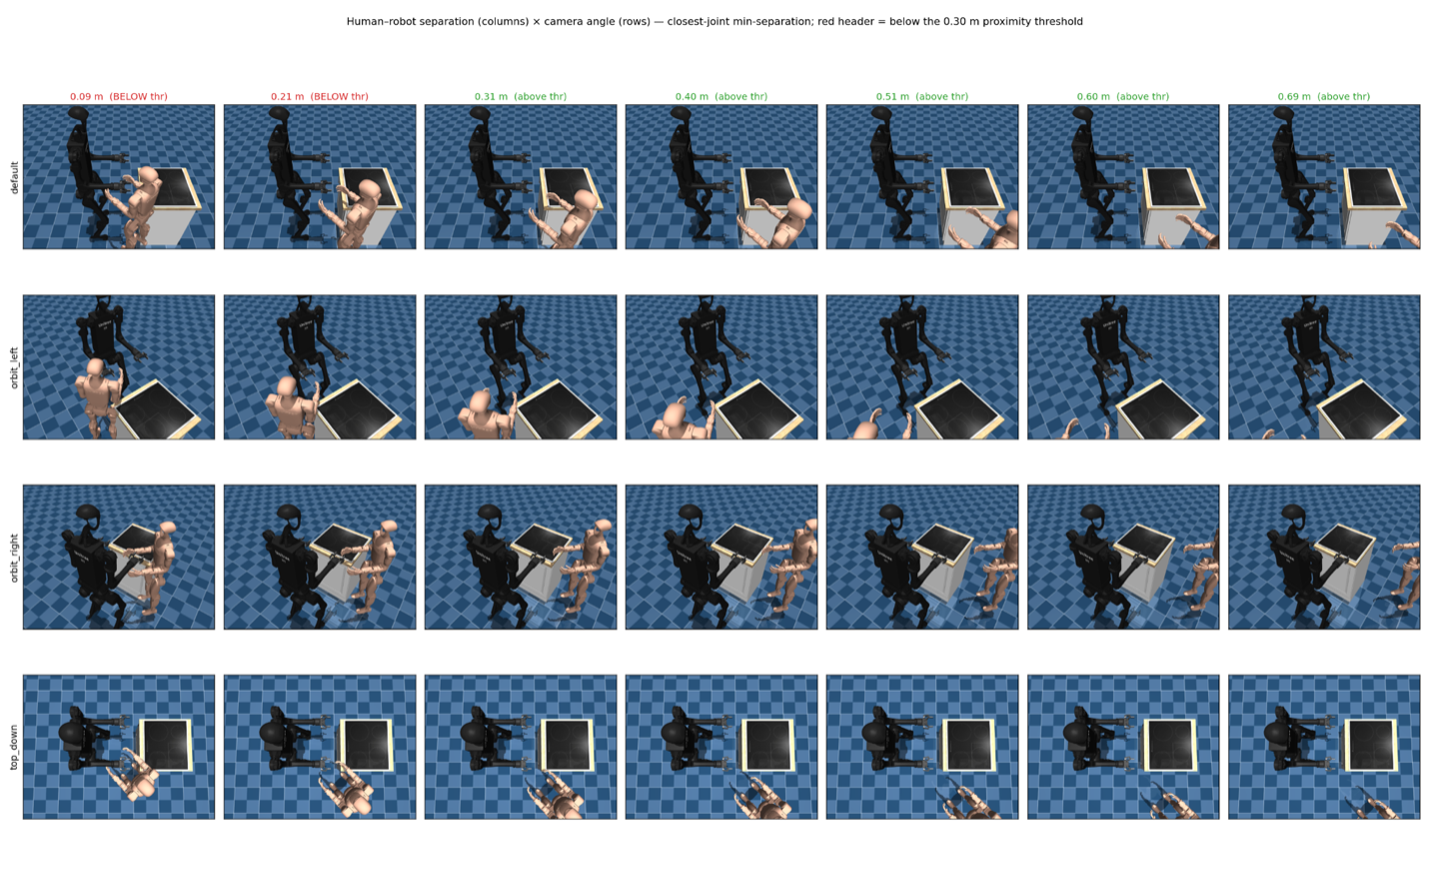
\includegraphics[width=0.62\textwidth]{separation_render_grid.png}
\caption{Contact-geometry calibration of $\tau_{\mathrm{prox}}$. The
H1 robot (dark) and the G1 coworker (light) are rendered at seven
controlled closest-joint separations (columns) from four camera angles
(rows), with the \texttt{saucepan\_to\_hob} table between them. Red
column headers are below the $0.30$\,m proximity threshold: at $0.09$
and $0.21$\,m the body geometries visibly interpenetrate, whereas by
$0.31$\,m (green) a clear gap has opened. This confirms that $0.3$\,m
sits just above the physical contact band, so a proximity violation
fires \emph{before} contact.}
\label{fig:separation-scale}
\end{figure}

\paragraph{Empirical distribution.}
The second check uses the observed distribution of closest-pair
separations. For any threshold $\tau$, the proximity-violation rate is
the empirical cumulative distribution function (CDF)
$P(\min\text{-separation} < \tau)$. In plain terms, it is the fraction
of steps whose closest separation is below $\tau$.

Table~\ref{tab:prox-calib} reports this fraction for a representative
unconstrained robot policy with the G1 coworker used during benchmark calibration
(3 seeds, 20 episodes, 30{,}000 steps). The rate rises gradually from
$0.2$ to $0.3$\,m, then starts to absorb more benign mid-range
proximity as the threshold moves to $0.5$ and $1.0$\,m. This supports
$0.3$\,m as an early-warning threshold: it captures near-contact
behaviour without counting most ordinary co-location as a violation.

\begin{table}[htbp]
\centering
\small
\caption{Proximity-violation rate as a function of the threshold
$\tau$ (the empirical CDF of $\min$-separation on a representative
unconstrained robot policy with the G1 coworker, 3 seeds $\times$ 20 episodes,
30{,}000 steps). A $0.3$\,m threshold captures the near-contact band
without absorbing as much benign mid-range proximity as $0.5$\,m or
$1.0$\,m.}
\label{tab:prox-calib}
\begin{tabular}{lccccccc}
\toprule
$\tau$ (m) & 0.20 & \textbf{0.30} & 0.40 & 0.50 & 0.60 & 0.75 & 1.00 \\
\midrule
Violation rate & 20.1\,\% & \textbf{25.3\,\%} & 29.9\,\% & 35.8\,\% & 39.5\,\% & 47.0\,\% & 62.9\,\% \\
\bottomrule
\end{tabular}
\end{table}

We fix $\tau_{\mathrm{prox}} = 0.3$\,m. It is above the contact band,
but still close enough to focus on near-contact behaviour. Because the
threshold is purely geometric, it is independent of robot speed. The
same proximity-violation rate can therefore be compared across
policies, tasks, and disruption bands. This threshold is held fixed in
every experiment in the report.

\section{Continuous Cost Signals}
\label{sec:bench:cost}

The wrapper computes two continuous, anticipatory cost signals from
the \iso{} margins:
\begin{align}
  c^{\ssm}_t  &= \max\!\left(0,\; 1 - \frac{m^{\ssm}_t}{d_{\mathrm{buffer}}}\right),
    \label{eq:c-ssm} \\
  c^{\pfl}_t  &= \max\!\left(0,\; f^{\mathrm{ratio}}_t - 0.8\right),
    \label{eq:c-pfl} \\
  c_t         &= \min\!\left(1,\; \max(c^{\ssm}_t,\, c^{\pfl}_t)\right),
    \label{eq:c-total}
\end{align}
where $m^{\ssm}_t$ is the instantaneous \ssm{}-actual margin
(positive when safe, negative when violating), $d_{\mathrm{buffer}}
= 0.3$\,m is the anticipation buffer, and $f^{\mathrm{ratio}}_t$ is
the force-ratio from Equation~\ref{eq:iso-pfl-ratio}. The
aggregator takes the worst-case across both criteria and saturates
at $c_t = 1$.

\paragraph{Why continuous rather than binary.}
A binary indicator $c_t \in \{0,1\}$ on violation supplies only
\emph{post-hoc} gradient signal. The policy learns that crossing
the threshold is bad but receives no information about how close to
the threshold it is approaching. The continuous formulation in
Equations~\ref{eq:c-ssm}--\ref{eq:c-pfl} gives a non-zero cost
before violations occur: a \ssm{}-actual margin of $0.15$\,m carries
a cost of $\sim$0.5, and any margin beyond the $0.3$\,m buffer
carries zero. We adopt it for this gradient richness. We note in
advance, however, that the cost-signal \emph{form} turns out
\emph{not} to be the operative variable: Experiment~E3.1
(Section~\ref{sec:results:cost-signal}) shows that at a tight budget
both the continuous and the binary forms collapse, because the
binding quantity is the Lagrangian budget relative to the task's
inherent cost, not the encoding of the cost. The continuous form is
retained as the more principled design, not because it is shown to
dominate the binary one.

The choice of $d_{\mathrm{buffer}} = 0.3$\,m matches the typical
\iso{}~\ssm{} robot-stopping contribution at the H1's observed
end-effector speeds. The 0.8 threshold in Equation~\ref{eq:c-pfl}
matches the 20\,\% headroom that \iso{} Annex~A motivates for
``approaching the limit''.

\paragraph{The \pfl{} contact-detection limitation.}
\pfl{} flag computation reads MuJoCo's \texttt{data.ncon} for
human--robot contact pairs. \bigym{}'s runtime robot-attachment in
\textsc{mojo} currently produces \texttt{data.ncon = 0} for these
pairs despite geometric overlap, so $c^{\pfl}_t \equiv 0$ throughout
the project. The wrapper exposes a \texttt{use\_pfl} flag wired
through every component. The flag can be flipped on once the
contact-detection issue is resolved without architectural change.
\textbf{All quantitative compliance claims in this report are
qualified as \ssm{}/proximity-only}
(Section~\ref{sec:disc:pfl-bug}).

\section{The \coworker{} Disruption: Design and Rationale}
\label{sec:bench:coworker}

The dominant deployment pattern for human-aware manipulation is
\emph{sustained co-working}. The human is in the workspace for the
whole task, not only for a one-shot intrusion. This is the situation a
household robot in a kitchen would face. The original \bigym{}
distribution had no human at all. Earlier \sbigym{} disruption types
encoded only one intrusion event per episode, which is too narrow for
this setting. We introduce \textsc{Disruption.coworker} as the primary
distribution for both training and evaluation.

\subsection{Design Goals}
\label{sec:bench:coworker:design}

The \coworker{} disruption was designed against three concrete
targets:

\begin{enumerate}[topsep=2pt,itemsep=2pt]
\item \emph{Realism.} The human's behaviour should resemble what a
  real co-worker would do in a shared kitchen: enter the workspace,
  approach the task area, occasionally reach toward the task object
  or toward the robot's own arm, and occasionally step
  away for a moment. Episodes should feel like minutes of
  collaboration, not seconds of intrusion.
\item \emph{Sufficient disruption to expose unsafe behaviour.} If
  the human's reaches are rare or always far from the robot, a
  fast-but-careless policy is safe by luck and the benchmark cannot
  discriminate. The \coworker{} band tightens the closest
  \emph{pelvis-to-pelvis} approach (0.60--0.95\,m) and the
  \textsc{near} dwell (9--14\,s). This distance is measured between
  body centres, not between the closest body parts. When the coworker
  reaches, the arm can move well inside the pelvis-to-pelvis distance,
  so closest-pair separations can still enter the
  $\tau_{\mathrm{prox}} = 0.3$\,m zone. The
  resulting baseline
  \texttt{ep\_proximity\_violation\_rate} of $0.296$
  (Section~\ref{sec:results:baseline}) is high enough to expose a
  $20+\,\%$ improvement as statistically significant.
\item \emph{Compositional disruption modes.} A real co-worker
  exhibits at least three distinct behaviours over a session:
  staying put while reaching; walking in then staying; walking in,
  leaving briefly, and returning. The \coworker{} sampler covers all
  three but weights them unequally, drawing the most demanding mode
  (patrol) the large majority of the time so that the training
  distribution concentrates on the hardest behaviour while still
  exercising the simpler ones.
\end{enumerate}

\subsection{Three Trajectory Modes}
\label{sec:bench:coworker:traj}

A \coworker{} scenario samples one of three trajectory modes. The
patrol mode is drawn $\sim$90\,\% of the time. The two simpler modes
share the remaining $\sim$10\,\%:

\begin{description}[leftmargin=2em,topsep=2pt,itemsep=2pt]
\item[\textsc{stationary}] G1 spawns at \textsc{near} distance and
  stays put. Arm reaches throughout the episode.
\item[\textsc{approach-loiter-depart}] G1 spawns far, walks in to
  \textsc{near}, stays put. Arm reaches after arrival.
\item[\textsc{coworker-patrol}] G1 walks in to \textsc{near}, then
  cyclically departs to an \textsc{away} position (90°--270°
  offset, $\sim$2--3\,m), loiters, returns to a \emph{new}
  \textsc{near} position (different angle, slightly different
  distance), and repeats. Arm reaches only while at \textsc{near}.
\end{description}

The patrol mode is the dominant mode at full strength because it
creates a realistic rhythm of interruption and opportunity. When the
coworker is near, the robot must handle close co-working. When the
coworker departs to the \textsc{away} position, the robot has a window
to continue the task. The two simpler modes are retained as occasional
variety in the headline distribution and as the bulk of the earlier
curriculum stages (Section~\ref{sec:method:curriculum}), which ramp up
to the patrol-dominant mixture.

Appendix~\ref{app:patrol-episode} (Figure~\ref{fig:coworker-patrol})
walks through one complete patrol episode frame by frame: the reach
cycles at \textsc{near} drive the closest-pair separation below
$\tau_{\mathrm{prox}}$, the \textsc{away} excursion restores a safe
margin, and the return starts the cycle again.

\subsection{Arm State Machine and Reach Gate}
\label{sec:bench:coworker:arm}

Independently of trajectory, the G1's reaching arm runs a four-state
cycle, \textsc{extend} $\to$ \textsc{hold} $\to$ \textsc{retract}
$\to$ \textsc{idle} (fractions $0.15/0.20/0.15/0.50$ of a period
$T \in [1.3, 2.2]$\,s in the train band), sampling per cycle whether
to reach for the robot's end-effector or the task object
(\texttt{target\_mix\_p\_ee}), with the target re-resolved each step
so the reach tracks a moving robot. A \emph{reach gate} suppresses
the IK during patrol's \textsc{away} phase. Because the arm idles
half of each cycle and patrol periodically vacates the \textsc{near}
zone, the task remains completable throughout: the success-rate axis
rewards progress in those windows over a trivial ``freeze until the
human leaves'' strategy.

\subsection{Train and Eval Parameter Spaces}
\label{sec:bench:coworker:params}

Five \coworker{} axes are exposed as continuous
\texttt{ParameterSpace} ranges, with train and eval distributions
configured separately for the OOD generalisation experiment (E5.2):

\begin{table}[htbp]
\centering
\small
\caption{The \coworker{} train and eval \texttt{ParameterSpace}.
Train is moderately tight, deliberately set to produce a high
baseline violation rate (so a $20+\,\%$ safety improvement is
statistically detectable). Eval is wider, capturing the
generalisation question. Closest approach is measured pelvis to pelvis.
The 0.60\,m floor is the smallest body-centre distance that keeps the
G1 mocap-pelvis collision capsule clear of the H1 pelvis collision
capsule. Proximity violations below 0.3\,m are still possible because
the reaching arm can move inside this body-centre distance.}
\label{tab:coworker-params}
\begin{tabular}{lcc}
\toprule
Axis & Train (\texttt{coworker\_train}) & Eval (\texttt{coworker\_eval}) \\
\midrule
Closest-approach distance     & $0.60$--$0.95$\,m  & $0.6$--$1.8$\,m  \\
Reach period $T$              & $1.3$--$2.2$\,s    & $3.0$--$9.0$\,s  \\
$P(\text{reach EE})$          & $0.45$--$0.72$     & $0.1$--$0.9$     \\
Near-loiter dwell time        & $9.0$--$14.0$\,s   & $4$--$16$\,s     \\
Walk speed                    & $1.0$--$1.4$\,m/s  & $0.6$--$2.2$\,m/s\\
\bottomrule
\end{tabular}
\end{table}

\section{The Task Suite: Three Tasks, Two Co-location Regimes}
\label{sec:bench:task}

The evaluation uses three \bigym{} tasks:
\texttt{saucepan\_to\_hob}, \texttt{dishwasher\_close}, and
\texttt{drawers\_open\_all}. They are all treated as full benchmark
tasks. The suite was chosen to satisfy three requirements:

\begin{enumerate}[topsep=2pt,itemsep=2pt]
\item \textbf{Long horizon for violation opportunity.}
  The tasks last long enough for the coworker to approach, reach,
  leave, and return. Short reach-target tasks often end before the
  coworker has cycled enough to expose representative unsafe
  behaviour.
\item \textbf{Workspace overlap with the coworker.} The saucepan
  pickup, dishwasher handle, and drawer handles all lie inside the
  H1's manipulation workspace. They are also plausible targets for the
  coworker's reaching arm. Episode trajectories therefore pass through
  the same volume the coworker occupies, exposing meaningful \ssm{}
  and proximity violations rather than incidental closeness.
\item \textbf{\bigym{}-RL competence.} Of the four candidate
  \bigym{} tasks we screened, these three support competent
  unconstrained \cqnas{} baselines after the curriculum
  (Section~\ref{sec:method:curriculum}). This matters because any
  safety improvement should be measured against a policy that can
  already do the task, not against a failing controller. \cqnas{}
  task-performance on \bigym{} is documented in~\cite{seo2024cqnas}.
\end{enumerate}

\paragraph{Two co-location regimes.}
Although all three tasks run under the same \coworker{} distribution,
their geometry produces different co-location patterns. This
difference turns out to govern which safety mechanism works
(Chapter~\ref{ch:eval}). On \texttt{saucepan\_to\_hob}, the
coworker's reach destination overlaps the robot's working volume for
most of the episode. The co-location is \emph{persistent}: the closest
geometry pair sits inside the interaction envelope almost
continuously. On \texttt{dishwasher\_close} and
\texttt{drawers\_open\_all}, close encounters arrive in \emph{bursts}.
The coworker's patrol cycle and the appliance-facing geometry leave
genuinely-safe windows between approaches. This is \emph{intermittent}
co-location. The distinction is not asserted from task descriptions
alone. Section~\ref{sec:results:boundary} measures it using the
activity rate of a separation-triggered runtime filter. That is the
operational definition used throughout: persistent means the filter
would be active most of the time, while intermittent means it would
not.
Figure~\ref{fig:task-suite} shows the three settings at a
close-approach instant.

\begin{figure}[htbp]
\centering

\includegraphics[width=\textwidth]{task_suite}
\caption{The three-task suite, photographed mid-episode from live
task executions under the
\coworker{} disruption: the Unitree H1 manipulator (black) shares
its working volume with the Unitree G1 human-coworker stand-in
(light) in the \bigym{} kitchen. Left: \texttt{saucepan\_to\_hob},
whose pick-and-place trajectory and the coworker's reach destination
coincide, so co-location is \emph{persistent}. Centre and right:
\texttt{dishwasher\_close} and \texttt{drawers\_open\_all}, where
close encounters arrive in bursts separated by genuinely-safe
windows (\emph{intermittent} co-location). The annotated separation
is the environment's ground-truth closest-pair distance at the
pictured instant; the same coworker distribution drives all three
tasks, so the regime is a property of the task--coworker pair, not
of the disruption.}
\label{fig:task-suite}
\end{figure}

\section{Mock \bodyslampp{}: Calibrated Perception Noise}
\label{sec:bench:perception}

Real robots do not know the human's true position. They estimate it
from sensors. To model this perception gap, \sbigym{} exposes a
configurable \texttt{BodySLAMWrapper} with three modes:

\begin{description}[leftmargin=2em,topsep=2pt,itemsep=2pt]
\item[\texttt{off}] No human-state channel in the observation.
\item[\texttt{oracle}] Ground-truth human position is injected as
  \texttt{human\_pos\_estimate} (6D: position + occluded flag +
  staleness counter + confidence).
\item[\texttt{noisy}] The full mock-\bodyslampp{} pipeline is calibrated
  against the published noise characteristics ~\cite{henning2023bodyslampp}.
\end{description}

The noisy mode applies four effects:
\begin{enumerate}[topsep=2pt,itemsep=1pt]
\item Temporally-correlated position noise
  ($\alpha = 0.9$, $\sigma = 0.05$\,m, stationary std $\approx
  0.115$\,m), calibrated against \bodyslampp{}'s reported
  positional accuracy~\cite{henning2023bodyslampp}.
\item 3-step latency buffer ($\approx 60$\,ms at 50\,Hz control,
  matching the 15+\,FPS perception clock typical of monocular
  visual-inertial pose estimation).
\item Stochastic tracking dropout ($p = 0.02$/step) with staleness
  counter; OU state continues to update during dropout, so
  recovery is smooth rather than discontinuous.
\item Optional ray-cast occlusion from the H1's head camera.
\end{enumerate}

\paragraph{Demo-replay path.}
Cached \bigym{} demonstrations~\cite{chernyadev2024bigym} were
recorded \emph{without} a coworker. Their
\texttt{human\_pos\_estimate} channel would therefore be missing if
read live. The wrapper supports a \texttt{mode=demo\_replay} path that
synthesises \texttt{human\_pos\_estimate} from an
\texttt{AMASSDemoPositionProvider}~\cite{mahmood2019amass} playing
back a real motion clip. Behaviour-cloning pretraining therefore sees
realistic human state at training time without a train--evaluation
distribution shift on this channel.

\section{Demonstrations and the Demo-Conversion Pipeline}
\label{sec:bench:demos}

\cqnas{}~\cite{seo2024cqnas} needs demonstrations. Without them,
long-horizon manipulation runs rarely discover the sparse task reward.
The benchmark therefore includes a demo-conversion path.

The conversion has three steps. First, it loads the cached \bigym{}
demonstrations from the raw, non-safety-wrapped environment, which is
the format expected by \bigym{}'s \texttt{DemoStore}. Second, it
converts each demonstration into the \texttt{ExtendedTimeStep} format
used by \cqnas{}. Third, it adds the human-state channel expected by
\sbigym{}. The original demos contain no coworker, so the converter
synthesises \texttt{human\_pos\_estimate} from an AMASS motion clip and
sets a safe-side placeholder cost $c_t = 0$.

One implementation detail is important for reproducibility. \cqnas{}
normalises actions using statistics computed from demonstrations. The
live environment must use those same demo-derived statistics. If it
does not, the policy learns one action scale from the demos and
executes another scale during rollout. Section~\ref{sec:impl:integration}
describes this integration fix.
% =============================================================================
% PART III: A HYBRID SAFETY ARCHITECTURE (the solution)
% =============================================================================

% =============================================================================
\chapter{Methods: The Two Parts of the Hybrid Safety Critic}
\label{ch:method}
% =============================================================================

\section{Overview: Two Parts, One Open Question}
\label{sec:method:overview}

Chapter~\ref{ch:benchmark-env} introduced \sbigym{} as the
benchmark and Section~\ref{sec:bench:why} listed six concrete
properties the benchmark is designed to test. The unconstrained
\cqnas{}~\cite{seo2024cqnas} baseline that ships with \bigym{}
fails almost all six: it has no representation of human position,
no \ssm{} margin, no constraint that would distinguish a
task-completing trajectory from one that endangers the coworker,
and Section~\ref{sec:results:baseline} will show that it registers
proximity violations on $\approx$30\,\% of steps (mean separation only
$0.13$\,m, with the worst approaches within a few millimetres), far
above what any plausible co-working deployment would accept.

This chapter presents the Hybrid Safety Critic, the architecture used
to close that gap. It turns the unconstrained imitation-or-RL policy
into an \iso{}-aware collaborator. The architecture has two mechanisms
with different roles:

\begin{enumerate}[topsep=2pt,itemsep=2pt]
\item A \textbf{training-time mechanism} that \emph{internalises}
  safety into the policy via a value-based Lagrangian formulation
  of the continuous cost signal. At deployment, the policy is
  used as-is; the safety knowledge is baked into the learned
  $Q$-functions (Section~\ref{sec:method:lagrangian}).
\item A \textbf{deployment-time mechanism}: a runtime \emph{filter
  slot} that intercepts the policy's proposed actions. The slot is
  mechanism-agnostic. We evaluate four ways to fill it: an
  offline-trained, frozen safety value function (SVF) used as a veto
  (Section~\ref{sec:method:filter}); two closed-form alternatives, a
  graded \iso{} speed-scaling rule and a model-based geometric dodge
  (Section~\ref{sec:method:filter:closedform}); and
  \emph{critic-gated speed-scaling}. In the last design, the SVF
  decides \emph{when} to intervene and the graded scaler decides
  \emph{how} (Section~\ref{sec:method:filter:gated}).
\end{enumerate}

Both mechanisms share a network shape and an observation interface.
This keeps the two safety critics comparable and leaves SVF reuse
available as an option. In the reported runs, however, the constrained
policy's cost critic is cold-started
(Section~\ref{sec:method:lagrangian:warmstart}). The mechanisms differ
in training objective and operational role. Figure~\ref{fig:hybrid-overview}
sketches the deployment pipeline. This chapter leaves one question
open: \emph{which mechanism should carry the safety burden in a given
deployment?} The results answer that question with the regime map.

Table~\ref{tab:method-final-choices} summarises the final design
choices. The rest of this chapter explains the alternatives that were
tested before reaching these choices.

\begin{table}[htbp]
\centering
\small
\caption{Final architecture choices used in the headline evaluations.
The alternatives are still described because they are part of the
evidence for the regime map.}
\label{tab:method-final-choices}
\renewcommand{\arraystretch}{1.15}
\begin{tabular}{@{}
    >{\raggedright\arraybackslash}p{0.19\textwidth}
    >{\raggedright\arraybackslash}p{0.35\textwidth}
    >{\raggedright\arraybackslash}p{0.34\textwidth}@{}}
\toprule
Component & Final choice & Why \\
\midrule
Policy-side safety & Dual reward/cost critics & Uses reward and safety cost without an actor network \\
Multiplier & Fixed $\lambda = 0.1$ & More stable than PID at the feasible budget boundary \\
Runtime backstop & Speed-scaling, optionally critic-gated & Slows smoothly instead of hard-vetoing actions \\
Persistent regime & Constrained policy carries exposure safety & Filters fire too often and freeze or flee \\
Intermittent regime & Critic-gated speed-scaling carries velocity safety & Safe windows let the gate preserve throughput \\
\bottomrule
\end{tabular}
\end{table}

\begin{figure}[htbp]
\centering
\resizebox{\textwidth}{!}{%
\begin{tikzpicture}[
  >=Latex, node distance=10mm and 11mm,
  box/.style={draw, rounded corners, align=center, inner sep=4pt,
              minimum height=11mm, font=\small},
  env/.style={box, fill=black!5},
  pol/.style={box, fill=blue!8, draw=blue!55, minimum width=42mm},
  filt/.style={box, fill=orange!12, draw=orange!70, minimum width=34mm},
  trn/.style={box, dashed, fill=black!3, draw=black!45, align=center,
              font=\footnotesize, text=black!75, minimum height=10mm},
  flow/.style={->, thick},
  tflow/.style={->, thick, dashed, black!55},
]
% deployment row
\node[env] (env) {Environment\\[-1pt]{\footnotesize \textsc{BiGym} $+$ G1 coworker}};
\node[box, right=of env] (obs) {Observation $s_t$\\[-1pt]{\footnotesize proprio.\ $+\ \hat p_{\mathrm{human}}$}};
\node[pol, right=of obs] (pol) {Policy $\pi$\\[2pt]$a^{\mathrm{nom}}=\mathrm{argmax}_{a}[\,Q_r-\lambda Q_c\,]$};
\node[filt, right=of pol] (filt) {Runtime filter\\[2pt]$Q_{\mathrm{safe}}(s,a^{\mathrm{nom}})\ge R$\,?};
\node[box, right=of filt] (exec) {Execute $a_t$};

\draw[flow] (env) -- (obs);
\draw[flow] (obs) -- (pol);
\draw[flow] (pol) -- (filt);
\draw[flow] (filt) -- node[above,font=\footnotesize]{pass}
                      node[below,font=\footnotesize]{$a_t{=}a^{\mathrm{nom}}$} (exec);

% veto branch
\node[box, fill=orange!5, draw=orange!55, font=\footnotesize,
      minimum height=8mm, below=9mm of filt] (fb) {fallback $a^{\mathrm{fb}}$};
\draw[flow] (filt.south) -- node[right,font=\footnotesize]{veto} (fb.north);
\draw[flow] (fb.east) -| (exec.south);

% feedback loop
\draw[flow] (exec.north) -- ++(0,7mm) -| (env.north);

% training band
\node[trn, below=15mm of pol] (lag)
  {trained \emph{online}: value-based\\ Lagrangian on cost $c_t$
   $\;\Rightarrow\; Q_r,Q_c$};
\node[trn, below=15mm of fb] (cql)
  {trained \emph{offline} (CQL),\\ frozen at deployment
   $\;\Rightarrow\; Q_{\mathrm{safe}}$};
\draw[tflow] (lag) -- (pol);
\draw[tflow] (cql.north) -- (filt.west);
\end{tikzpicture}%
}
\caption{The Hybrid Safety Critic at deployment: a two-part
architecture. At each step the Lagrangian-trained policy proposes the
nominal action
$a^{\mathrm{nom}} = \mathrm{argmax}_a\,[Q_r(s,a) - \lambda Q_c(s,a)]$;
a runtime filter slot passes it through when its safety check holds
and otherwise modifies or replaces it (veto, dodge, graded
speed-scaling, or critic-gated speed-scaling,
Sections~\ref{sec:method:filter}--\ref{sec:method:filter:gated}). The
two parts have different jobs: the constrained policy
internalises safety \emph{proactively} during training, while the
filter is a \emph{reactive} runtime mechanism. Chapter~\ref{ch:eval}
shows that which part carries the safety burden is governed by the
co-location regime: under persistent co-location only the policy
reduces exposure gracefully
(Table~\ref{tab:e4.1-feature-incremental}), while under intermittent
co-location the critic-gated filter is the working part
(Section~\ref{sec:results:r2-gated}).}
\label{fig:hybrid-overview}
\end{figure}

\section{The Offline Safety Value Function}
\label{sec:method:filter}

\subsection{Dataset and Labelling}
\label{sec:method:filter:data}

The SVF is trained offline on transitions collected by rolling out
\cqnas{} policy snapshots from the base-policy curriculum
(Section~\ref{sec:method:curriculum}). Collection uses the
\coworker{} distribution and the \texttt{noisy} observation mode.
Earlier critics mixed random-policy and demonstration transitions. The
current critic uses policy snapshots alone. This is because the filter
must be accurate in the regions a deployed policy actually visits.
Snapshot rollouts sample that distribution, including the mistakes a
competent-but-imperfect policy makes under sustained co-working. The
filter is \emph{noisy-native}: it is trained and evaluated on
\texttt{noisy} human-state estimates. On ground-truth
(\texttt{oracle}) input its $Q$-estimates collapse and it intervenes
almost everywhere. For that reason, all filtered evaluations are
reported on \texttt{noisy}
(Section~\ref{sec:setup:perception-mode}). The current critic contains
37{,}883 transitions. Of these, $16.8\,\%$ are labelled unsafe
($r^{\mathrm{safe}} = 0$) at the $\tau = 0.3$\,m proximity threshold.
The full figures are in the repository's filter-training write-up.

Each transition is labelled with the binary safety reward
\begin{equation}
  r^{\mathrm{safe}} \;=\; 1 - \mathbb{1}[\texttt{proximity\_violation}],
  \label{eq:r-safe}
\end{equation}
using the geometric proximity-violation flavour of
Section~\ref{sec:bench:metrics:flavours} at the calibrated threshold
$\tau_{\mathrm{prox}} = 0.3$\,m (the calibration is derived in
Section~\ref{sec:bench:proximity-threshold}). We label on
\texttt{proximity\_violation} rather than
\texttt{ssm\_violation\_actual} for two reasons. First, the
conservative-ISO \ssm{} flag is saturated. It fires on $\sim$93\,\% of
random rollouts and remains high even for competent policies, because
it assumes the worst-case human velocity. It carries almost no useful
gradient for a value function. Second, labelling on geometry keeps the
two safety mechanisms separate. The runtime filter is responsible for
the \emph{geometric} danger of being too close. The velocity-dependent
\ssm{} response is left to the cost signal and the constrained policy
(Section~\ref{sec:method:lagrangian}). If the filter's label depended
on instantaneous velocity, it would also depend on the action the
filter is meant to judge. That would conflate ``how dangerous is this
configuration'' with ``how fast is the robot moving''. The latter is a
policy decision.

Because the violating class is the minority, a
\texttt{WeightedRandomSampler} over-samples it to a $1{:}1$ ratio of
safe to violating transitions per batch, so the critic is not
dominated by the safe majority.

\paragraph{A shared critic for the intermittent-co-location tasks.}
\texttt{dishwasher\_close} and \texttt{drawers\_open\_all} use a
second SVF trained once across both tasks. This critic is
\emph{task-agnostic}: its inputs are robot proprioception, the
estimated human position, and the proposed action. They do not include
the task name. The same input format is valid on both tasks, so a
single critic can learn a local safety question: ``is this action
dangerous given where the human is?''

This shared critic is used only as a \emph{gate} for speed-scaling in
the intermittent regime. Its job is not to label every moment of close
co-location as bad. Its job is to identify near-contact moments where
the speed-scaler should switch on. For that reason it is labelled at
$0.10$\,m rather than at the benchmark's $0.30$\,m proximity threshold.
The $0.30$\,m threshold remains the report's exposure metric
(Section~\ref{sec:bench:proximity-threshold}). The tighter $0.10$\,m
label makes the gate more selective, so safe close-passing windows can
still be used for task progress. The dataset contains 52{,}794
transitions collected from curriculum-policy rollouts on both tasks
under \coworker{} disruption. Ablations with earlier-warning
$0.20$\,m and $0.30$\,m labels confirm that the selective near-contact
label is the better gate (Section~\ref{sec:results:r2-ablations}).

\subsection{Architecture and Training}
\label{sec:method:filter:arch}

The safety critic is a 3-layer MLP with hidden sizes
$[256, 256, 256]$ and ReLU activations. The input is the
concatenation of robot proprioception, the mock-\bodyslampp{} 6D
human-position estimate, and the proposed action. The output is
bounded to $[0, q_{\max}]$ with $q_{\max} = 1/(1-\gamma)$ via a
scaled sigmoid, which \emph{mathematically} prevents Bellman
overestimation: $Q$ cannot exceed the maximum possible discounted
return of a safe trajectory.

Training combines a Bellman residual with the
\textsc{CQL}~\cite{kumar2020cql} regulariser:
\begin{equation}
  \mathcal{L} \;=\; \mathcal{L}_{\mathrm{Bellman}}
  \;+\; \alpha_{\mathrm{CQL}} \cdot
  \left(\mathbb{E}_{a \sim \mathrm{uniform}}\!\left[Q(s,a)\right]
       - \mathbb{E}_{a \sim \mathcal{D}}\!\left[Q(s,a)\right]\right),
  \label{eq:cql-loss}
\end{equation}
with $\alpha_{\mathrm{CQL}} = 5.0$ as the headline value, Polyak
target update $\tau = 0.005$. Full training hyperparameters in
Appendix~\ref{app:hparams:svf}.

\subsection{No-Pixel Critic: Justification}
\label{sec:method:filter:nopixels}

The filter does not consume RGB, for three reasons: \emph{compute}
(a pure-MLP critic costs $\sim$0.3\,ms per forward against a
$\sim$20\,ms control budget, versus a substantial CNN-encoder
fraction); \emph{robustness} (no lighting/texture domain shift, only
the upstream pose estimator's
calibration~\cite{henning2023bodyslampp}); and
\emph{compositionality} (a no-pixel filter wraps any policy whose
observation includes proprioception, the human-position estimate,
and the proposed action).

\subsection{Runtime Wrapper}
\label{sec:method:filter:runtime}

At deployment, the \texttt{SafetyFilterWrapper} intercepts the
proposed action and compares the safety value against a threshold
$R$:
\begin{equation}
  a^{\mathrm{exec}}_t \;=\;
  \begin{cases}
    a^{\mathrm{nom}}_t   & \text{if } Q_{\mathrm{safe}}(s_t, a^{\mathrm{nom}}_t) \ge R, \\
    a^{\mathrm{fb}}_t    & \text{otherwise.}
  \end{cases}
  \label{eq:filter-rule}
\end{equation}
$R$ is calibrated by sweep over a held-out validation set
(Experiment~E2.3, Section~\ref{sec:results:filter-pareto}); the
headline operating point for the G1 critic on the \coworker{}
distribution is $R = 2.25$. The intended role of the veto at this
operating point is an \iso{}~\ssm{} \emph{velocity backstop} rather
than a proximity reducer: much of the residual proximity is the
human walking up to an otherwise stationary robot, which no veto of
robot actions can prevent; Section~\ref{sec:results:filter-pareto}
quantifies the resulting limits.

The veto's fallback is zero-velocity braking on the floating base
and on every joint velocity actuator. This can produce abrupt
motion mid-trajectory; proportional damping is the natural upgrade
and is deferred to future work (Section~\ref{sec:fw:fallback}).

\section{Closed-Form Runtime Filters: Speed-Scaling and Geometric Dodge}
\label{sec:method:filter:closedform}

The filter slot in Figure~\ref{fig:hybrid-overview} is
mechanism-agnostic. Any rule that maps the state and proposed action
$(s_t, a^{\mathrm{nom}}_t)$ to an executed action can occupy it. The
learned SVF veto above is the learned version. Two \emph{closed-form}
mechanisms complete the reactive taxonomy evaluated in
Chapter~\ref{ch:eval}: stop (veto), slow (speed-scaling), and move
away (dodge). Both closed-form filters consume the same
$\hat{p}^{\mathrm{human}}$ estimate as the SVF and contain no learned
component.

The point of this section is to define the runtime options that are
tested later. Table~\ref{tab:runtime-options} gives the comparison set.
The final runtime mechanism is not assumed here; it is selected by the
results.

\begin{table}[htbp]
\centering
\small
\caption{Runtime filter options evaluated in the report. They differ
in what they do after detecting risk.}
\label{tab:runtime-options}
\begin{tabular}{lll}
\toprule
Option & Response & Purpose of the test \\
\midrule
SVF veto & stop & tests a learned binary override \\
Speed-scaling & slow & tests the graded \ssm{} response \\
Geometric dodge & move away & tests whether reactive retreat helps \\
Critic-gated speed-scaling & decide when, then slow & tests selective use of the graded response \\
\bottomrule
\end{tabular}
\end{table}

\subsection{Graded \iso{} Speed-Scaling}
\label{sec:method:filter:speedscale}

\iso{}~\ssm{}'s intent is graded: the robot should \emph{slow} as
separation shrinks, not merely stop at a threshold. The speed-scaling
filter implements this directly. At each step a scale factor is
computed from the closest-pair human--robot separation
$\mathrm{sep}_t$,
\begin{equation}
  \sigma_t \;=\; \mathrm{clip}\!\left(
    \frac{\mathrm{sep}_t - d_{\mathrm{stop}}}
         {d_{\mathrm{slow}} - d_{\mathrm{stop}}},\; 0,\; 1\right),
  \qquad
  a^{\mathrm{exec}}_t \;=\; q_t + \sigma_t \,
    \bigl(a^{\mathrm{nom}}_t - q_t\bigr),
  \label{eq:speed-scale}
\end{equation}
where $q_t$ is the current joint position for the absolute-mode arm
dimensions (so the per-step \emph{motion} from the current pose is
scaled) and zero for the delta-mode floating base (so the commanded
increment is scaled directly). Above $d_{\mathrm{slow}}$ the filter
is the identity ($\sigma_t = 1$, the action is unchanged); at or
below $d_{\mathrm{stop}} = 0.15$\,m the robot holds position
($\sigma_t = 0$); in between, speed falls linearly with separation.
The slow radius $d_{\mathrm{slow}}$ is the single operating-point
knob, swept over $[0.25, 0.60]$\,m with the headline at $0.40$\,m;
an intervention is any step with $\sigma_t < 1$. Unlike the veto,
this filter preserves the \emph{direction} of the policy's motion
and modulates only its magnitude, which is why it can maintain the
graded velocity margin the standard prescribes where a binary
stop-or-go veto cannot
(Section~\ref{sec:results:headline-feature-table}).

\subsection{Model-Based Geometric Dodge}
\label{sec:method:filter:dodge}

The second closed-form mechanism is a geometric
control-barrier-style fallback: when the closest-pair separation
falls below a target $d_{\mathrm{target}}$, the filter adds a
correction step directed \emph{away} from the human, proportional to
the violation depth $(d_{\mathrm{target}} - \mathrm{sep}_t)$ and
capped per step. Two variants differ in which part of the robot
dodges: the \emph{base-dodge} pushes the floating base along the
escape direction and leaves the arm untouched, while the
\emph{end-effector retract} (``flinch'') keeps the base planted and
retracts the end-effector along the escape direction via a
damped-Jacobian step. $d_{\mathrm{target}}$ is swept over
$[0.30, 0.55]$\,m. These variants exist to test whether a
\emph{dodging} reactive response escapes the limits of the
\emph{stopping} one; Section~\ref{sec:results:reactive-taxonomy}
shows it does not (it trades the veto's freeze for a flee). The
veto and the dodges are reported as taxonomy points
(Table~\ref{tab:filter-taxonomy}), with operating-point values for
all mechanisms in Appendix~\ref{app:hparams:hybrid}.

\subsection{Critic-Gated Speed-Scaling: The Runtime Mechanism}
\label{sec:method:filter:gated}

The unconditional speed-scaler of
Section~\ref{sec:method:filter:speedscale} pays its task cost at
\emph{every} close approach. This includes cases that are genuinely
safe: the human may be close but stationary, moving away, or near a
barely moving robot. The learned SVF of
Section~\ref{sec:method:filter} can distinguish some of these cases.
The binary veto is the wrong way to use that information. The
\emph{critic-gated speed-scaling} filter therefore splits the decision:

\begin{equation}
  a^{\mathrm{exec}}_t \;=\;
  \begin{cases}
    a^{\mathrm{nom}}_t
      & \text{if } Q_{\mathrm{safe}}(s_t, a^{\mathrm{nom}}_t) \ge R
        \quad\text{(critic says safe: full speed)}, \\
    q_t + \sigma_t\,(a^{\mathrm{nom}}_t - q_t)
      & \text{otherwise}
        \quad\text{(critic flags risk: graded slow-down, Eq.~\ref{eq:speed-scale})}.
  \end{cases}
  \label{eq:gated-rule}
\end{equation}

The critic decides \emph{when} to intervene. The speed-scaler decides
\emph{how}. Both halves matter. Replacing the graded slow-down with a
hard veto breaks the action coherence of a chunked policy
(Section~\ref{sec:results:r2-veto}). Removing the gate makes the
scaler fire on every close approach and pay the full unconditional
task cost. The gate threshold $R$ is the operating-point dial:
$R \to 0$ recovers the unfiltered policy, $R \to \infty$ recovers
unconditional scaling, and intermediate values trace a frontier
between them (Section~\ref{sec:results:r2-gated}). The
regime-dependent question is whether that frontier bends toward a
high-success, low-violation corner or merely slides between its two
endpoints. Section~\ref{sec:results:boundary} answers that question.

\section{The Value-Based Lagrangian Constrained Policy}
\label{sec:method:lagrangian}

\subsection{Why Value-Based}
\label{sec:method:lagrangian:why}

\cqnas{}~\cite{seo2024cqnas} is \emph{critic-only}: the policy is
implicit, $\pi(s) = \mathrm{argmax}_{a \in
\mathcal{A}_{\mathrm{bin}}} Q(s, a)$, over a coarse-to-fine
discretisation of the joint action space. The classical
actor-critic Lagrangian formulation~\cite{ray2019safetygym,
stooke2020pid} updates a policy network $\pi_\theta$ to maximise
$\mathbb{E}[Q_r(s,a)] - \lambda \mathbb{E}[Q_c(s,a)]$, which
presumes that $\pi_\theta$ exists as a separately-trained network.
There is no $\pi_\theta$ in \cqnas{}. The Lagrangian must be
re-expressed in value-based form.

The starting point is the constrained objective
\begin{equation}
  \max_{\pi} J_r(\pi)
  \quad \text{s.t.} \quad
  J_c(\pi) \le d,
  \qquad
  J_r(\pi)=\mathbb{E}_{\pi}\!\left[\sum_t \gamma^t r_t\right],
  \quad
  J_c(\pi)=\mathbb{E}_{\pi}\!\left[\sum_t \gamma^t c_t\right].
  \label{eq:cmdp-objective}
\end{equation}
For any fixed multiplier $\lambda \ge 0$, the Lagrangian relaxation is
$\mathcal{L}(\pi,\lambda)=J_r(\pi)-\lambda(J_c(\pi)-d)$. The
$\lambda d$ term is constant with respect to action choice. A
critic-only policy can therefore implement the same trade-off at
decision time by learning separate action-values
\[
Q_r(s,a)\approx\mathbb{E}\!\left[\sum_t\gamma^t r_t\mid s_0=s,a_0=a\right],
\qquad
Q_c(s,a)\approx\mathbb{E}\!\left[\sum_t\gamma^t c_t\mid s_0=s,a_0=a\right],
\]
and selecting the action that maximises $Q_r-\lambda Q_c$. This is the
key reproducibility point: \emph{the policy improvement step is
changed, not the Bellman target of the reward critic}. The reward and
cost critics can therefore be trained on stationary targets. The
multiplier $\lambda$ acts only as a deployment-time or training-time
selection parameter.

Three options were considered. They are listed from simplest to most
principled. The choice is also tested empirically (Experiment~E3.1).

\subsection{Option A-value: Shaped-Reward Single Critic}
\label{sec:method:lagrangian:A}

The simplest formulation folds the cost into a modified reward and
trains a single critic:
\begin{equation}
  r^{\mathrm{mod}}_t \;=\; r^{\mathrm{task,shaped}}_t \;-\; \lambda \cdot c_t,
  \qquad
  Q(s,a) \approx \mathbb{E}\!\left[\sum_t \gamma^t r^{\mathrm{mod}}_t\right],
  \label{eq:option-A}
\end{equation}
with action selection $a^* = \mathrm{argmax}_a Q(s,a)$. Its weakness is
that the regression target is \emph{non-stationary} in $\lambda$.
The multiplier is itself non-stationary because it tracks rolling
cost. The critic therefore chases a moving target. This option is used
only as a prototype baseline.

\subsection{Option B-value-mean: Dual Q-Functions on Mean Cost (Headline)}
\label{sec:method:lagrangian:Bmean}

Decouple the reward and cost critics:
\begin{align}
  Q_r(s,a) &\approx \mathbb{E}\!\left[\sum_t \gamma^t r^{\mathrm{task,shaped}}_t\right], \\
  Q_c(s,a) &\approx \mathbb{E}\!\left[\sum_t \gamma^t c_t\right],
\end{align}
each regressing toward its own \emph{stationary} target. The action
selection combines them at decision time:
\begin{equation}
  a^* \;=\; \mathop{\mathrm{argmax}}_{a \in \mathcal{A}_{\mathrm{bin}}}
  \Big[\,Q_r(s,a) \;-\; \lambda \cdot Q_c(s,a)\,\Big].
  \label{eq:Bmean-select}
\end{equation}
$\lambda$ now enters only at selection, not at regression. The
cost critic shares its network shape with the offline SVF, so SVF
reuse is available, though here the cost critic is cold-started
(Section~\ref{sec:method:lagrangian:warmstart}). This is the
\textbf{headline architecture} for this work.


\subsection{Option B-value-CVaR: Distributional Cost Critic (future work)}
\label{sec:method:lagrangian:Bcvar}

A natural extension replaces the mean-cost critic with a
distributional one: $Q_c$ is replaced by either a Gaussian
parametrisation $(\mu_c, \sigma_c)$~\cite{yang2021wcsac} or a
quantile head $\{\theta_k\}_{k=1}^K$~\cite{dabney2018qrdqn}, with
action selection
\begin{equation}
  a^* \;=\; \mathop{\mathrm{argmax}}_{a \in \mathcal{A}_{\mathrm{bin}}}
  \Big[\,Q_r(s,a) \;-\; \lambda \cdot \cvar_{\alpha}(Z_c \mid s, a)\,\Big],
\end{equation}
with $\alpha \in \{0.95, 0.99\}$. This would align training with the
\cvar{} evaluation metric and answer the standard critique that
mean-cost methods bound only $\mathbb{E}[Z_c]$; the cost head is
already C51-shaped, but calibrating a rolling-\cvar{} target and
re-verifying the support invariant
(Section~\ref{sec:method:lagrangian:support}) for the cost
distribution requires careful engineering. \textbf{We adopt
B-value-mean as the headline and defer explicit-\cvar{} training to
future work (Section~\ref{sec:fw:cvar})}, evaluating the
mean-policy's \emph{achieved} \cvar{} as a diagnostic
(Section~\ref{sec:results:tail}).

\subsection{The C51 Value-Support Invariant}
\label{sec:method:lagrangian:support}

\cqnas{} uses a C51 distributional reward critic with fixed value
support $[v_{\min}, v_{\max}]$~\cite{bellemare2017c51}. The Bellman
target is projected back onto that support at each update. This matters
for reward shaping. If a dense shaping term can produce a discounted
return outside the support, C51 clips it. Once clipped, very different
bad actions can look equally bad to the critic, because they all sit at
the lower support boundary. The shaping signal then stops being useful.

The design rule is simple: the worst possible discounted shaping
penalty must fit inside the negative side of the value support.

\begin{proposition}[Support-bounding invariant]
\label{lem:support-bound}
Let a C51 distributional critic have value support
$[v_{\min}, v_{\max}]$, discount $\gamma$, and an additive shaped
reward $r^{\mathrm{shaped}}_t \in [-\beta \cdot c_{\mathrm{ws}}, 0]$
with $\beta, c_{\mathrm{ws}} > 0$. The shaped-reward contribution
to the discounted return is bounded by
$\beta \cdot c_{\mathrm{ws}} / (1 - \gamma)$ in magnitude. The
Bellman target clamp is informative (i.e., the support is not
saturated) only if
\begin{equation}
  \beta \cdot c_{\mathrm{ws}} \,/\, (1-\gamma) \;\le\; |v_{\min}|.
  \label{eq:support-invariant}
\end{equation}
\end{proposition}

\begin{proof}
The geometric-series sum of the per-step shaping under the worst
case gives $\sum_{t=0}^\infty \gamma^t \beta c_{\mathrm{ws}} =
\beta c_{\mathrm{ws}} / (1-\gamma)$, and the C51 target clamp
clips below $v_{\min}$. \qed
\end{proof}

\paragraph{How it is used here.}
The benchmark uses the bounded workspace penalty from
Equation~\ref{eq:r-workspace}. We set $c_{\mathrm{ws}} = 1.0$\,m,
$\beta = 0.05$, $\gamma = 0.99$, and widen the reward support to
$[v_{\min}, v_{\max}] = [-6, +2]$. The worst-case shaping contribution
is therefore $0.05 \cdot 1.0 / 0.01 = 5$, which fits inside the
negative support because $5 \le 6$. This check is why the bounded
workspace shaping can be added without saturating the critic. The same
check applies to any distributional critic with dense reward shaping.

\subsection{Per-Env-Step Cost Backup}
\label{sec:method:lagrangian:per-step}

\cqnas{} executes \emph{action sequences} of length $K$ between
policy queries (coarse-to-fine refinement). A natural but subtly
wrong design is to backup the cost critic on the chunk-averaged
cost $\bar{c} = (1/K) \sum_{k} c_{t+k}$. The policy can satisfy a
mean-over-chunk budget while spiking violations \emph{inside} a
chunk. The cost critic must be backed up on \emph{every} env-step's
$c_t$. Our training pipeline preserves $c_t$ through the replay
buffer at per-env-step granularity
(Section~\ref{sec:impl:integration}).

\subsection{PID Lagrange Multiplier Update}
\label{sec:method:lagrangian:pid}

The standard Lagrangian approach tunes the multiplier $\lambda$
automatically. We test the PID controller of
Stooke et al.~\cite{stooke2020pid} because it is a common choice for
safe RL. Here $d$ is the target cost budget: the maximum average
episode cost the policy is meant to stay below. Let $m_t$ be the
rolling per-episode cost mean. The PID update is
\begin{align}
  e_t &= m_t - d, \\
  \lambda_{t+1} &= \mathrm{clip}\!\left(\lambda_t + K_I \cdot e_t
    + K_P \cdot e_t + K_D \cdot (e_t - e_{t-1}),
    \; 0,\; \lambda_{\max}\right).
  \label{eq:pid-lambda}
\end{align}
PID is designed to adjust $\lambda$ upward when recent cost is above
the budget and downward when the policy is safely below it. We use
$K_I = 10^{-3}$, $K_P = 10^{-2}$, $K_D = 0$, and
$\lambda_{\max} = 100$ in the PID ablation.

\paragraph{Why PID is not the headline setting.}
The task's inherent mean cost is $\approx$0.25--0.30. Any budget
$d \le 0.2$ is therefore infeasible, because abandoning the task is the
only way to stay under it. A budget of $d = 0.5$ is slack and drives
$\lambda \to 0$. The single viable budget, $d = 0.3$, sits at the
task's inherent cost. At that boundary, small differences between
training seeds matter. Here, ``seeds'' means independent training runs
with different random initialisation, replay sampling, and environment
randomness.

Across three seeds at $d = 0.3$, PID converged to three very different
multipliers: $\lambda = 0.000$, $0.267$, and $3.855$. These produced an
unconstrained policy, a useful avoidance policy, and a collapsed policy
respectively. Section~\ref{sec:results:budget} presents the evidence
with the budget sweep (Figure~\ref{fig:lambda-regimes}).

For the headline experiments, we therefore do \emph{not} use PID
auto-tuning. We keep the cost critic $Q_c$ and the dual-action
selection rule, but fix $\lambda$ manually. Sweeping fixed values makes
$\lambda$ a clear proximity--success knob, and the headline setting is
$\lambda = 0.1$ (Figure~\ref{fig:fixlam}). The conclusion is not that
PID is a bad algorithm in general. It is that, in this task, the only
useful budget lies too close to the natural cost floor for PID to tune
reliably.

\subsection{Filter During Training (optional)}
\label{sec:method:lagrangian:filter-train}

The runtime safety filter of Section~\ref{sec:method:filter} can
also be applied at training time, interposed between the proposed
action and the environment, vetoing catastrophically unsafe
proposals with the fallback~\cite{cbfrl2024,shield2025}. We report
results without the training-time filter as the default; the
filter-during-training ablation is deferred to future work
(Section~\ref{sec:fw:filter-during-training}).

\subsection{Cost-Critic Initialisation and Policy Warm-Start}
\label{sec:method:lagrangian:warmstart}

Two initialisation choices matter here, and they point in opposite
directions. The actor, the reward critic and the shared visual encoder
are \emph{warm-started} from the unconstrained base policy: the
stage-1 snapshot of the curriculum
(Section~\ref{sec:method:curriculum}) is loaded so that constrained
training begins from a task-competent policy rather than from scratch.
The cost critic $Q_c$, by contrast, is \emph{cold-started} (freshly
initialised).

This is deliberate. Although $Q_c$ shares its network shape with the
offline SVF, the two carry opposite sign conventions ($Q_c$ high
means dangerous, $Q_{\mathrm{safe}}$ high means safe) and different
learning targets (offline CQL value of a binary proximity label vs.\
online expected value of the continuous cost under the current
policy); seeding $Q_c$ from the SVF would initialise it on a surface
the dual-Q selection step would have to unlearn. A
\texttt{warm\_start\_from\_svf} path (with the required sign-flip)
remains in the codebase, unused in the reported runs. One loader
subtlety matters for reproduction: the unconstrained base
snapshot contains no cost-critic keys, so the loader guards them
explicitly, task weights load, $Q_c$ stays freshly initialised.


\section{External Baseline: Worst-Case SAC}
\label{sec:method:wcsac}

To position the value-based Lagrangian against published safe-RL work,
not only against our own ablations, we reimplement
WCSAC~\cite{yang2021wcsac}. WCSAC is the
canonical distributional safe actor-critic. We run it on the same
76-DOF tasks (\texttt{agent=wcsac} on the same training stack). WCSAC
maintains a Gaussian distributional cost critic and constrains
$\cvar_{\alpha}$ of the discounted cost return ($\alpha = 0.9$) to a
budget $d$ through an adaptively tuned multiplier.

The comparison is not like-for-like. Our main agent is
demonstration-driven and value-based. WCSAC is actor-critic and, in its
standard form, does not use the \cqnas{} demonstration warm-start. We
therefore train WCSAC from scratch
($\text{num\_demos} = 0$, 150k frames) and report it as an external
reference point, not as a direct ablation of our architecture. Results
are in Section~\ref{sec:results:r2-lagrangian}.

\section{The Base-Policy Curriculum}
\label{sec:method:curriculum}

Direct training on the full \coworker{} disruption distribution from a
randomly initialised \cqnas{} agent fails. The base policy learns to
evacuate the workspace within 5--10k frames and never attempts the
task. \texttt{ep\_reward} stays at the floor and
\texttt{success\_rate} stays at 0. The cause is a
\emph{distribution-shift cascade}. Cached \bigym{} demonstrations
contain no coworker, so behaviour cloning teaches ``go to the task,
ignore everything''. At runtime, the live coworker physically blocks
the task path and produces off-distribution states. The C51 critic has
no reliable signal in those states, so the policy drifts toward
whatever physics and workspace shaping favour. In practice, that is
away from the human and toward the workspace boundary.

The fix is a three-stage curriculum that resumes from each prior
stage's snapshot~\cite{narvekar2020curriculum}. The environment is
\emph{stateless} with respect to training step, so the curriculum
is implemented as three sequential training runs with snapshot
resume. The \texttt{BodySLAMWrapper} channel and the obs width are
preserved across stages by keeping a coworker in the scene at all
stages (just distant in stage~0), so the architecture and replay
buffer carry over cleanly.

\begin{table}[htbp]
\centering
\small
\caption{The three-stage coworker curriculum. The task stays the same;
only the coworker's behaviour becomes more intrusive.}
\label{tab:curriculum-stages}
\begin{tabular}{llll}
\toprule
Stage & Disruption & Coworker behaviour & Frames \\
\midrule
0 & \texttt{coworker\_idle} & G1 present, distant, no reaching & 30k \\
1 & \texttt{coworker\_easy} & moderate distance, occasional reaches & 30k \\
2 & \texttt{coworker\_train} & full patrol and reach band from Table~\ref{tab:coworker-params} & 40k \\
\bottomrule
\end{tabular}
\end{table}

Stages~0--1 establish task competence before the full coworker
distribution is introduced. Stage~2 then trains and evaluates the base
policy on the real disruption band used by the safety experiments.

\paragraph{Why a curriculum (against alternatives).}
The failure mode is not lack of randomisation. It is that the agent
does not discover the task reward when the full coworker is present
from the first update. Domain randomisation on human speed would make
the human behaviour more varied, but it would not solve this discovery
problem. Curriculum learning is the appropriate tool because it first
teaches the task, then increases the coworker difficulty.

Empirically, stages~0--1 learn the task reliably, with
\texttt{ep\_reward} around $+1.8$. Direct training on the full
\coworker{} band instead diverges and evacuates the workspace. Stage~2
then serves two purposes: it produces the unconstrained baseline on the
real distribution, and it provides the warm-start for the constrained
Lagrangian policy.


\section{Algorithm}
\label{sec:method:algorithm}

\begin{algorithm}[H]
\caption{The value-based Lagrangian training loop (headline
dual-critic, mean-cost formulation). Because the backbone is
critic-only, the constraint enters through action selection on
$Q_r - \lambda Q_c$ rather than through an actor update: both
critics train on stationary Bellman targets, the cost critic is
backed up at per-env-step granularity, and $\lambda$ is fixed in the
headline configuration because PID auto-tuning is seed-unstable at
the feasibility boundary (Section~\ref{sec:results:budget}).}
\label{alg:constrained-rl}
\begin{algorithmic}[1]
\Require Task reward $r^{\mathrm{task,shaped}}_t$ (workspace shaping
  per Equation~\ref{eq:r-workspace}), cost signal $c_t$ per
  Equation~\ref{eq:c-total}, cost budget $d$, PID gains
  $(K_P, K_I, K_D)$, optional offline filter $Q_{\mathrm{safe}}$ +
  threshold $R$
\State Warm-start the actor, reward critic $Q_{r,\phi_r}$ and
  encoder from the stage-1 curriculum snapshot; initialise the cost
  critic $Q_{c,\phi_c}$ from scratch (cold start)
\State Initialise replay buffer, demo replay buffer; load
  $\text{num\_demos}$ demonstrations
\State $\lambda \leftarrow \lambda_0$ \Comment{headline: fixed
  $\lambda_0 = 0.1$ (PID gains zero); PID-tuned only in the
  seed-instability ablation}
\For{each environment step $t$}
  \State $a^{\mathrm{nom}}_t \leftarrow \mathrm{argmax}_{a \in
  \mathcal{A}_{\mathrm{bin}}}\!\big[Q_r(s_t,a) - \lambda \cdot
  Q_c(s_t,a)\big]$
  \If{using training-time filter \textbf{and}
  $Q_{\mathrm{safe}}(s_t, a^{\mathrm{nom}}_t) < R$}
    \State $a_t \leftarrow a^{\mathrm{fb}}_t$ \Comment{fallback}
  \Else
    \State $a_t \leftarrow a^{\mathrm{nom}}_t$
  \EndIf
  \State Step env; store $(s_t, a_t, r^{\mathrm{task,shaped}}, c,
    s_{t+1})$ in replay
  \State Sample batch (demos + replay)
  \State Update $\phi_r$: C51 Bellman regression on
    $r^{\mathrm{task,shaped}}$ per-env-step
  \State Update $\phi_c$: Bellman regression on $c$ per-env-step
  \If{episode end \textbf{and} PID-tuning $\lambda$ (ablation only)}
    \State $m \leftarrow$ rolling mean cost over recent episodes;
      \quad $e \leftarrow m - d$
    \State $\lambda \leftarrow \mathrm{clip}(\lambda + K_I e
      + K_P e + K_D (e - e_{\mathrm{prev}}),\; 0,\; \lambda_{\max})$
  \EndIf
  \Statex \hspace{\algorithmicindent}\textit{(headline runs keep
    $\lambda \equiv \lambda_0$; see
    Section~\ref{sec:method:lagrangian:pid})}
\EndFor
\end{algorithmic}
\end{algorithm}


% =============================================================================
% (merged) The sections below were formerly Chapter 6 "Implementation
% Details". They are now the implementation half of this chapter.
% =============================================================================

\section{Software Architecture and Metric Provenance}
\label{sec:impl:arch}
\label{sec:impl:metrics}

Table~\ref{tab:software-architecture} summarises the implementation.
The important provenance point is that every reported number comes from
the same snapshot-evaluation harness. The training loop writes costs
into replay at per-environment-step granularity, and the benchmark
harness later produces one CSV row per evaluation cell.

\begin{table}[htbp]
\centering
\small
\caption{Software components relevant to the reported experiments.}
\label{tab:software-architecture}
\begin{tabular}{lll}
\toprule
Component & Main files / module & Role in the report \\
\midrule
Benchmark env & \texttt{safety\_bigym/envs} & H1 robot, G1 coworker, task wrapper \\
Safety signals & \texttt{safety\_bigym/safety} & \ssm{}, proximity, and \pfl{} metric schema \\
Perception wrapper & \texttt{BodySLAMWrapper} & oracle/noisy human-position estimates \\
Offline filter & \texttt{safety\_bigym/filters} & SVF dataset, critic, runtime wrapper \\
\cqnas{} agent & \texttt{safety\_bigym/agents/cqn\_as} & adapter, reward critic, cost critic \\
Training entrypoint & \texttt{train\_cqn\_as.py} & curriculum and Lagrangian training \\
Evaluation harness & \texttt{benchmark\_policy.py} & canonical CSV rows for all result tables \\
\bottomrule
\end{tabular}
\end{table}

Configuration is managed with Hydra. Weights \& Biases (W\&B) is used
as the experiment-tracking website: training curves, evaluation
success, safety metrics, run names, tags, and checkpoints are logged
there so runs can be compared while experiments are still in progress.
For reproducibility, W\&B is not treated as the sole source of truth.
Each run also writes local JSONL metric dumps, and the benchmark
harness writes CSV rows for the final reported numbers. Training
targets a single NVIDIA A100 40\,GB GPU, and every script has a
CPU-only smoke gate.

\section{\cqnas{} Vendor Integration}
\label{sec:impl:integration}

The upstream \cqnas{}~\cite{seo2024cqnas} implementation was adapted
so that the same agent can train and evaluate inside \sbigym{}. The
integration has three report-relevant requirements:

\begin{enumerate}[topsep=2pt,itemsep=2pt]
\item \textbf{API compatibility.} \bigym{} exposes a Gym-style
  environment, while \cqnas{} expects \texttt{ExtendedTimeStep}
  objects. The adapter converts observations, rewards, discounts,
  actions, and costs into the format used by the agent.
\item \textbf{Human-state compatibility.} Cached \bigym{}
  demonstrations contain no coworker. Demo replay therefore injects a
  synthetic \texttt{human\_pos\_estimate} channel, so pretraining and
  live rollout have the same observation keys.
\item \textbf{Cost provenance.} The adapter carries per-step safety
  cost into replay as \texttt{ExtendedTimeStep.cost}. This is what
  allows the cost critic to train on the same safety signal that the
  benchmark later reports.
\end{enumerate}

Low-level compatibility fixes, version pins, and GPU-specific
diagnostics are documented in the repository. They are not needed to
understand the method, but they make the released code reproducible.

\section{Making the Offline Filter Deployment-Faithful}
\label{sec:impl:svf-faithful}

An offline safety filter must be trained on the same kind of state and
action distribution it will see at deployment. Otherwise, a validation
sweep can look good while the deployed filter behaves differently. For
this reason, SVF dataset collection uses the same control assumptions
as the benchmark harness.

Table~\ref{tab:deployment-faithful} lists the equivalence conditions we
enforce. They are methodological safeguards, not separate algorithmic
contributions.

\begin{table}[htbp]
\centering
\small
\caption{Deployment-faithfulness conditions for offline filter
collection. The filter is evaluated only after these conditions match
the benchmark harness.}
\label{tab:deployment-faithful}
\begin{tabular}{ll}
\toprule
Condition & Why it matters \\
\midrule
Same action scaling & The critic must score the actions the policy will actually execute \\
Same action execution mode & \cqnas{} uses action sequences and temporal ensembling at deployment \\
Same control frequency & Action effects and coworker motion depend on the control timestep \\
Same coworker scenario YAML & The collection distribution must match the reported benchmark distribution \\
Same noisy observation mode & The filter must see deployment-like human-state estimates \\
\bottomrule
\end{tabular}
\end{table}

The check is simple: with the filter disabled ($R = 0$), the SVF sweep
should reproduce the unfiltered benchmark baseline. It does:
the sweep proximity rate is $0.286$, close to the deployment benchmark
baseline of $0.296$. This agreement is the provenance check for the
filter results in Chapter~\ref{ch:eval}.



% =============================================================================
% PART IV: EVALUATION
% =============================================================================

% =============================================================================
\chapter{Evaluation Methodology: Tasks, Metrics, and Protocol}
\label{ch:protocol}
% =============================================================================

\section{Tasks}
\label{sec:setup:tasks}

The evaluation uses the three \bigym{} tasks introduced in
Section~\ref{sec:bench:task}. They are all full benchmark tasks. The
suite spans the two co-location regimes used by the regime map:
persistent co-location and intermittent co-location. Table~\ref{tab:eval-tasks}
summarises the tasks and their unconstrained baseline performance.

\begin{table}[htbp]
\centering
\small
\caption{Evaluation task suite. Baseline success is measured for the
unconstrained \cqnas{} policy under \coworker{} disruption and
\texttt{noisy} perception.}
\label{tab:eval-tasks}
\begin{tabular}{llll}
\toprule
Task & Manipulation type & Co-location regime & Baseline success \\
\midrule
\texttt{saucepan\_to\_hob} & pick, carry, place on hob & persistent & $0.85$ \\
\texttt{dishwasher\_close} & close appliance door & intermittent & $0.77$ \\
\texttt{drawers\_open\_all} & open drawers & intermittent & $0.82$ \\
\bottomrule
\end{tabular}
\end{table}

Unless stated otherwise, all headline evaluation uses the
\coworker{} distribution and \texttt{noisy} perception.

\section{Disruption Distributions}
\label{sec:setup:disruptions}

Training uses \texttt{Disruption.coworker} sampling from the
\texttt{coworker\_train} \texttt{ParameterSpace}
(Table~\ref{tab:coworker-params}). Evaluation uses the same
distribution for all in-distribution numbers and the wider
\texttt{coworker\_eval} distribution for the held-out
out-of-distribution (OOD) generalisation check
(Section~\ref{sec:results:ood}).

\section{Perception Mode (oracle vs.\ noisy)}
\label{sec:setup:perception-mode}

The \texttt{BodySLAMWrapper} of Section~\ref{sec:bench:perception}
defines three human-state observation modes: \texttt{off},
\texttt{oracle}, and \texttt{noisy}. The deployment-relevant setting is
\texttt{noisy}, so headline benchmark numbers use noisy evaluation.
Table~\ref{tab:perception-protocol} records the exact protocol.

\begin{table}[htbp]
\centering
\small
\caption{Perception protocol used in evaluation. WCSAC is flagged as
an external upper-bound reference because it is evaluated with oracle
human state.}
\label{tab:perception-protocol}
\begin{tabular}{lll}
\toprule
Component & Training / collection mode & Evaluation mode \\
\midrule
Constrained \cqnas{} policy & \texttt{oracle} & \texttt{noisy} \\
Offline SVF filter and gated sweeps & \texttt{noisy} & \texttt{noisy} \\
Perception ablation (E3.6) & same checkpoints & \texttt{oracle} and \texttt{noisy} \\
WCSAC external reference & \texttt{oracle} & \texttt{oracle} \\
\bottomrule
\end{tabular}
\end{table}

Training the policy on \texttt{oracle} isolates the effect of the
safety constraint. Training and evaluating filters on \texttt{noisy}
matches the deployment condition a runtime filter would face.

\section{Baselines and Configurations}
\label{sec:setup:baselines}

The results chapter evaluates four groups of configurations, all using
the same task and safety metrics.

\begin{description}[leftmargin=2em,style=nextline,itemsep=2pt]
\item[Persistent co-location: \texttt{saucepan\_to\_hob}.]
We compare the unconstrained baseline, the fixed-$\lambda$ constrained
policy, speed-scaling on the baseline, SVF vetoes, geometric dodges,
and the policy--filter composition. This tests whether safety has to
be trained into the policy.
\item[Intermittent co-location: \texttt{dishwasher\_close} and
\texttt{drawers\_open\_all}.]
We compare the unconstrained baseline, Lagrangian budget sweeps, SVF
vetoes, unconditional speed-scaling, and critic-gated speed-scaling.
This tests whether a runtime backstop can improve safety while
preserving throughput.
\item[Boundary test.]
We apply critic-gated speed-scaling to \texttt{saucepan\_to\_hob}, the
persistent task where the coworker stays near the robot's working
volume for much of the episode. This tests whether the
intermittent-regime recipe transfers.
\item[External reference.]
We evaluate WCSAC from scratch as a published safe-RL reference point.
\end{description}

\section{The Two Safety Axes and the Evaluation Protocol}
\label{sec:setup:metrics}

\subsection{The Exogenous Decomposition of Proximity}
\label{sec:setup:metrics:primary}
\label{sec:exogenous}

The protocol separates two safety axes. The first is
\texttt{ep\_proximity\_violation\_rate}: the fraction of steps with
closest human--robot separation below $0.3$\,m. The second is
\texttt{ep\_ssm\_violation\_actual\_rate}: the velocity-adaptive
\ssm{} violation rate under the realised human and robot velocities.

The split is needed because proximity is not fully robot-controlled. A
frozen-robot sweep shows that making the robot stop on every step
removes only $\approx$58\,\% of time-in-proximity
(Figure~\ref{fig:exogenous-decomposition}). The remaining
$\approx$42\,\% is the coworker approaching a robot that is already
stationary. Runtime filters cannot remove that part. They can,
however, control whether the robot moves too fast when the human is
near. Every results table therefore reports both proximity and
velocity-adaptive \ssm{}.

This floor is a limit on robot-controlled \emph{proximity}, not a
direct estimate of injury risk. Some exogenous close approaches may be
benign if the robot is stationary and contact forces stay below
\pfl{} limits. Because the current simulator does not expose reliable
human--robot contact forces, this report cannot determine which part of
the exogenous proximity floor would also be a \pfl{} violation.

\begin{figure}[htbp]
\centering
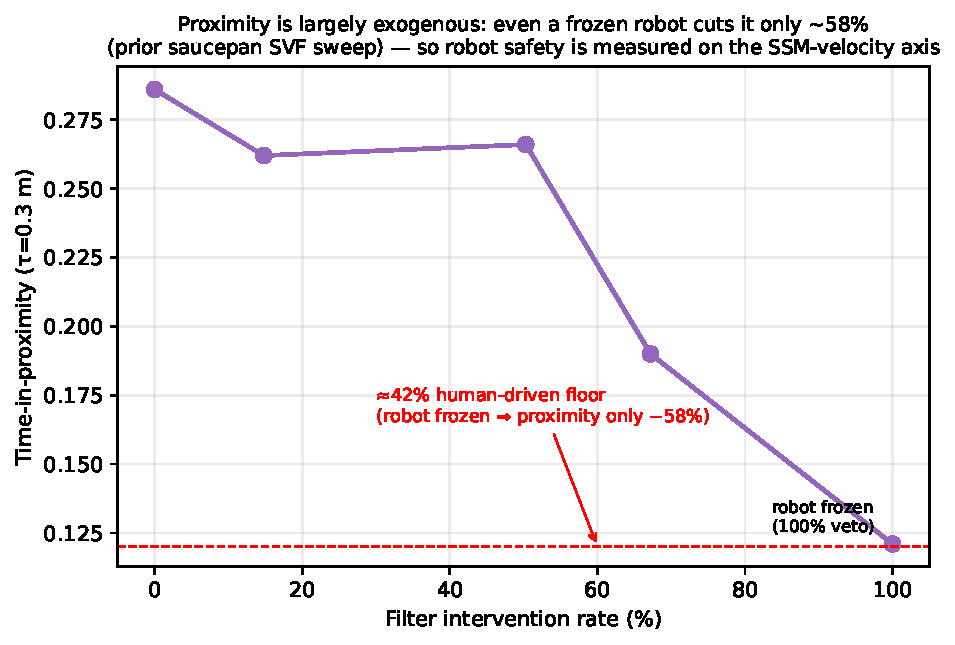
\includegraphics[width=0.62\textwidth]{fig4_exogenous_proximity}
\caption{The exogenous decomposition of proximity (the protocol's organising
measurement). Sweeping the runtime filter's intervention rate from
$0$ to $100\,\%$ (a fully frozen robot) removes only $\approx$58\,\%
of time-in-proximity; the residual $\approx$42\,\% is the coworker
approaching a stationary robot, a floor outside robot control. This is
a proximity floor, not a direct contact-injury estimate, because
\pfl{} forces are not available in the current simulator.
Provenance: this sweep is the \emph{prior} \texttt{saucepan\_to\_hob} SVF threshold
sweep, run before the intermittent-co-location experiments existed;
the two-axis protocol was fixed on its basis, not after seeing the
later results.}
\label{fig:exogenous-decomposition}
\end{figure}

\subsection{Axis Ownership}
\label{sec:setup:metrics:iso}

Table~\ref{tab:evaluation-metrics} gives the metrics used throughout
the results chapter. The conservative worst-case
\texttt{ep\_ssm\_violation\_rate} is kept for traceability, but it is
not the main decision metric because it saturates at $\sim$93\,\% on
random rollouts (Section~\ref{sec:bench:metrics:flavours}).

\begin{table}[htbp]
\centering
\small
\caption{Evaluation metrics and how they are interpreted.}
\label{tab:evaluation-metrics}
\resizebox{\textwidth}{!}{%
\begin{tabular}{llll}
\toprule
Axis & Metric & Main owner & Interpretation \\
\midrule
Task success & \texttt{success\_rate} & policy & terminal task completion \\
Task cost & \texttt{steps\_to\_completion} & policy/filter & slower but successful execution \\
Exposure & \texttt{ep\_proximity\_violation\_rate} & policy & fraction of steps below $0.3$\,m \\
Robot-controllable safety & \texttt{ep\_ssm\_violation\_actual\_rate} & runtime filter & robot moving too fast for the realised separation \\
Tail risk & $\cvar_{0.95}$ of \texttt{ep\_min\_separation} & diagnostic & worst-case closest approaches \\
Filter cost & \texttt{intervention\_rate} & runtime filter & fraction of steps modified by the filter \\
\bottomrule
\end{tabular}%
}
\end{table}

Three decision rules were fixed before the corresponding sweeps ran
(Table~\ref{tab:decision-rules}). They prevent the results from being
judged by a moving target.

\begin{table}[htbp]
\centering
\small
\caption{Pre-registered decision rules used to interpret the main
sweeps.}
\label{tab:decision-rules}
\renewcommand{\arraystretch}{1.2}
\begin{tabular}{@{}p{0.28\textwidth}p{0.36\textwidth}p{0.28\textwidth}@{}}
\toprule
Experiment & Rule & Purpose \\
\midrule
Observation ablation & $\geq 20\,\%$ \ssm{} reduction & tests whether observation alone helps \\
\addlinespace[3pt]
Reactive-filter sweep & $\geq 30\,\%$ proximity-violation reduction at $\leq 25\,\%$ intervention & tests graceful filtering \\
\addlinespace[3pt]
Boundary test on \texttt{saucepan\_to\_hob} & success $\geq 0.60$ and \ssm{}-actual $\leq 0.08$ & tests whether gating recovers throughput \\
\bottomrule
\end{tabular}
\renewcommand{\arraystretch}{1.0}
\end{table}

\subsection{Task Performance and the Safety Tax}
\label{sec:setup:metrics:task}

The safety tax is measured by comparing task performance against the
unconstrained baseline. The primary measure is
\texttt{success\_rate}. The secondary measure is
\texttt{steps\_to\_completion}, computed only among successful
episodes. A policy can be safe but slow, so both numbers are needed.

\texttt{episode\_reward} (sum of $r^{\mathrm{task,shaped}}_t$ over
the episode) is reported in appendix tables as a tertiary axis
that combines task progress and the workspace-shaping signal.

\subsection{Tail Risk}
\label{sec:setup:metrics:tail}

Tail-risk metrics ask whether the worst episodes remain dangerous even
when the mean improves. We report $\cvar_{0.95}$ of
\texttt{ep\_cost\_integral}, $\cvar_{0.95}$ of
\texttt{ep\_min\_separation}, and the 99\textsuperscript{th}
percentile of \texttt{ep\_min\_separation}. Each is computed over the
60 evaluation episodes in a cell unless a table states otherwise.
Contact-force tail metrics are not reported because of the open \pfl{}
contact-detection limitation (Section~\ref{sec:bench:cost}).

\subsection{Policy / Filter Interaction}
\label{sec:setup:metrics:interaction}

For runtime mechanisms, we also record \texttt{intervention\_rate}.
Its complement is passthrough rate: the fraction of steps where the
policy action is executed unchanged. During the internalisation
experiment, this rate is measured across intermediate policy
checkpoints to test whether the policy is learning to avoid situations
that trigger the filter.

\section{Statistical Methodology}
\label{sec:setup:stats}

Table~\ref{tab:experiment-overview} summarises the experiments before
the results chapter reports them. Appendix~\ref{app:exp-index} gives
the full repository-code mapping.

\begin{table}[htbp]
\centering
\small
\caption{Experiment overview used by the results chapter.}
\label{tab:experiment-overview}
\resizebox{\textwidth}{!}{%
\begin{tabular}{llll}
\toprule
Question & Experiments & Compared methods & Reported in \\
\midrule
Does human observation alone help? & E1.1 & behaviour cloning with/without human state & Section~\ref{sec:results:obs-bc} \\
Can constrained RL reduce exposure? & E3.1--E3.2, E4.1 & cost forms, budgets, fixed $\lambda$ & Section~\ref{sec:results:r1} \\
What can reactive filters do? & E2.1--E2.5, E4.3 & SVF veto, speed-scaling, dodge & Sections~\ref{sec:results:filter-pareto}--\ref{sec:results:interaction} \\
What works in intermittent co-location? & E3.3, E3.7, E2.6 & Lagrangian, WCSAC, gated speed-scaling & Section~\ref{sec:results:r2} \\
Where is the regime boundary? & E4.4 & critic-gated speed-scaling transferred to \texttt{saucepan\_to\_hob} & Section~\ref{sec:results:boundary} \\
Does the result survive noise/OOD/tails? & E3.6, E5.1--E5.2 & perception and distribution checks & Sections~\ref{sec:results:obs-rl}--\ref{sec:results:ood} \\
\bottomrule
\end{tabular}%
}
\end{table}

Every evaluation cell runs 20 episodes per evaluation seed across
three evaluation seeds (60 episodes), sampled from the relevant
\texttt{ParameterSpace}. Configurations involving a \emph{trained}
policy additionally pool three independently trained seeds, giving
180 episodes for the headline \texttt{saucepan\_to\_hob} policy and composition rows
and for every row of the boundary-condition sweep; each table states
which applies. 95\,\% bootstrap confidence intervals (CIs; 10{,}000
resamples over episodes) are reported for the headline safety
metric of each table. Directional claims are assessed by
bootstrap-CI overlap rather than parametric tests: episode-level
safety metrics are bounded, zero-inflated and heavily non-Gaussian,
so $t$-statistics would be poorly calibrated, whereas the CI
criterion is conservative and assumption-free. Two deliberate
exceptions to the three-trained-seed rule are flagged where they
occur: the intermittent-co-location Lagrangian budget sweep trains a
single seed per budget cell (six cells; the persistent-task sweep had already
established the seed-instability finding that would make per-cell
seed replication uninformative), and the WCSAC external reference is
a single seed per (task, budget) cell at 30 evaluation episodes,
reported with that caveat (Section~\ref{sec:results:wcsac}).

\label{sec:setup:smoke}%
Every script also carries a \texttt{--smoke} flag (a 5-minute CPU
validation); no multi-hour training was launched without passing the
relevant smoke gate first.

\section{Compute Budget}
\label{sec:setup:compute}

All training ran on single NVIDIA A100 (40\,GB) GPUs. The
persistent-co-location arc cost $\approx$220\,GPU-hours
(log-reconstructed), dominated by eighteen 40k-frame Lagrangian
fine-tunes at $\approx$9\,h each across the cost-form, budget, PID,
and fixed-$\lambda$ grids, plus the three-stage curriculum, the
confound control, the offline SVF pipeline, and snapshot evaluation.
The intermittent-co-location arc adds $\approx$230--280\,h, of which
the six 150k-frame from-scratch WCSAC runs dominate
($\approx$120--180\,h, estimated rather than log-reconstructed,
since they ran on a shared multi-GPU dispatcher). The project total
is roughly $450$--$500$\,GPU-hours; the carbon accounting
($\approx$40\,kg~CO\textsubscript{2}e under the 2024 UK grid
emissions factor) is derived in Appendix~\ref{app:sustainability}.


\section{The Unconstrained Baselines: Task-Competent, Not Compliant}
\label{sec:results:baseline}

This section establishes the unconstrained baseline against which later
improvements are measured. The baseline is task-competent on all three
tasks, but not safety-compliant under sustained co-working
(Table~\ref{tab:results:baseline}). The persistent task has the
highest success, but also substantial proximity and \ssm{} violations.

% [H]: pinned in place — as the last float of the chapter, [htbp] gets
% flushed by the \chapter pagebreak onto a lone, vertically-centred
% float page.
\begin{table}[H]
\centering
\caption{Unconstrained \cqnas{} baselines under \coworker{} disruption
and \texttt{noisy} perception. These are the ``before'' rows used for
all safety comparisons. Each cell uses 60 evaluation episodes.}
\label{tab:results:baseline}
\small
\begin{tabular}{lccc}
\toprule
Task & Success & Prox.\ viol. & \ssm{}-actual viol. \\
\midrule
\texttt{saucepan\_to\_hob}      & $0.85$ & $0.296$ & $0.146$ \\
\texttt{dishwasher\_close}      & $0.77$ & $0.246$ & $0.176$ \\
\texttt{drawers\_open\_all}     & $0.82$ & $0.211$ & $0.100$ \\
\bottomrule
\end{tabular}
\end{table}

\textbf{Reading.} The unconstrained baseline is the floor: a
task-competent policy that is \emph{not} \iso{} compliant under
sustained co-working. The deployment posture that \cqnas{}
ships with~\cite{seo2024cqnas} on \bigym{} would, under \sbigym{}'s
\coworker{} distribution, be within $0.3$\,m of the coworker on
$\approx$30\,\% of steps on the persistent task. Every reduction
reported below is relative to the relevant task's baseline.


% =============================================================================
% PART IV-B: RESULTS
% =============================================================================

% =============================================================================
\chapter{Results: Two Regimes, One Boundary}
\label{ch:eval}
% =============================================================================

\section{The Shape of the Evidence}
\label{sec:results:ablation-map}

This chapter reports the evaluation in three parts. The first
(Section~\ref{sec:results:r1}) studies the persistent-co-location
task, \texttt{saucepan\_to\_hob}. The second
(Section~\ref{sec:results:r2}) repeats the comparison on
\texttt{dishwasher\_close} and \texttt{drawers\_open\_all}. The third
(Section~\ref{sec:results:boundary}) tests the boundary between the
two regimes by transferring the intermittent-regime winner back to
\texttt{saucepan\_to\_hob}.

The evaluation is ablation-led. Each major component is removed,
replaced, or retuned to test whether it contributes. Table~\ref{tab:results-evidence-map}
summarises the logic of the chapter.

\begin{table}[htbp]
\centering
\small
\caption{How the main result is built from ablations. Each row tests a
specific explanation before the final regime map is stated.}
\label{tab:results-evidence-map}
\begin{tabular}{@{}p{0.23\textwidth}p{0.17\textwidth}p{0.27\textwidth}p{0.24\textwidth}@{}}
\toprule
Question & Experiment(s) & Key result & Conclusion \\
\midrule
Does human-state observation help by itself? & E1.1 & no cell meets the safety bar & safety needs a cost signal \\
What makes constrained RL bind? & E3.1--E3.2 & budget matters more than cost form & use fixed $\lambda$ near feasible cost \\
Can reactive filters reduce exposure? & E2.1--E2.3 & cheap vetoes do not reduce exposure & policy must handle persistent exposure \\
Which runtime action is usable? & E2.4--E2.5 & veto breaks; speed-scaling works & slow smoothly, do not hard-veto \\
Can a gate save throughput? & E2.6, E4.4 & yes when windows exist; no when persistent & co-location regime decides \\
\bottomrule
\end{tabular}
\end{table}

\section{Persistent Co-location: Safety Must Be Trained In}
\label{sec:results:r1}

This section covers the persistent-co-location side of the regime map. On
\texttt{saucepan\_to\_hob} the coworker occupies the robot's working
volume nearly continuously: a separation-triggered filter would be
active on $\approx$44--62\,\% of steps (measured directly in
Section~\ref{sec:results:boundary}). The claim this section
establishes is the first half of the regime map: \emph{where
co-location is persistent, no runtime mechanism reduces exposure
gracefully, but a fixed-multiplier constrained policy does}. It cuts
the proximity-violation rate by $23\,\%$ at $0.76$ success, reproducibly
across seeds. The evidence proceeds in order. Observation alone is not
a safety mechanism. The budget, not the cost form, makes the
constraint bind. Reactive filters help on the velocity axis but not on
the exposure axis. The headline comparison then shows the division of
labour and the composition's ceiling. The final subsections test the
result under perception noise, a held-out coworker distribution, and
the worst-case tail.

Here and below, a \emph{training seed} means an independent training run
with different random initialisation, replay sampling, and environment
randomness. A 95\,\% confidence interval (CI) is a bootstrap interval
over evaluation episodes.

\subsection{Human-State Observation Alone Is Not a Safety Mechanism}
\label{sec:results:obs-bc}

Here, ``observation'' means adding a human-state channel to the policy
input. The policy can either receive no human state
(\texttt{off}), ground-truth human state (\texttt{oracle}), or noisy
mock-\bodyslampp{} state (\texttt{noisy}). The experiment asks whether
this input alone makes a behaviour-cloned policy safer, before any
safety cost or constraint is added.

The result is negative. No observation setting met the pre-set success
criterion of a $20\,\%$ reduction in \ssm{} violations. The best case,
on \texttt{drawers\_open\_all}, reduced violations by only $13.7\,\%$.
On \texttt{saucepan\_to\_hob}, the oracle human-state channel made the
\ssm{} violation rate worse ($0.135 \to 0.203$), even though task
success improved ($0.22 \to 0.58$).

This shows that human-state observation is useful for task completion,
but not automatically for safety. The behaviour-cloned policy can use
the human channel to route around obstructions, yet it has no reason to
keep distance from the human. Safety needs an explicit cost or
constraint, not just an extra observation channel.

\subsection{The Cost Budget, Not the Cost Form, Is the Operative Variable}
\label{sec:results:cost-signal}
\label{sec:results:budget}

Two ablations locate what makes the constraint bind. E3.1 changes the
\emph{form} of the per-step cost: continuous graded cost versus a
binary indicator. Both are trained at a very tight budget,
$d=0.01$. Both collapse to $0\,\%$ task success. This means the failure
is not caused by the cost encoding. It is caused by the budget being
infeasible.

The reason is the exogenous cost floor. About $42\,\%$ of the
baseline's $0.296$ proximity-violation rate is caused by the human
approaching the robot (Section~\ref{sec:exogenous}). That alone implies
an achievable floor of roughly $0.12$, before considering any
robot-driven risk. A budget of $d=0.01$ is therefore impossible for any
useful task policy. The Lagrange multiplier grows, the cost term
dominates the task reward, and the policy abandons the task.

E3.2 then sweeps the budget $d$, the average cost target used by the
Lagrangian multiplier. Tight budgets
$d \in \{0.001, 0.05, 0.1\}$ again collapse task success
($0.00$, $0.00$, and $0.13$). The only useful region is near
$d=0.3$, close to the task's natural cost. At that boundary, PID
auto-tuning becomes seed-unstable: the three seeds converge to
$\lambda=0.000$, $0.267$, and $3.855$, producing an unconstrained
policy, a useful avoidance policy, and a collapsed policy. This is why
the headline policy fixes $\lambda$ manually instead of relying on PID
auto-tuning.

\begin{figure}[htbp]
\centering
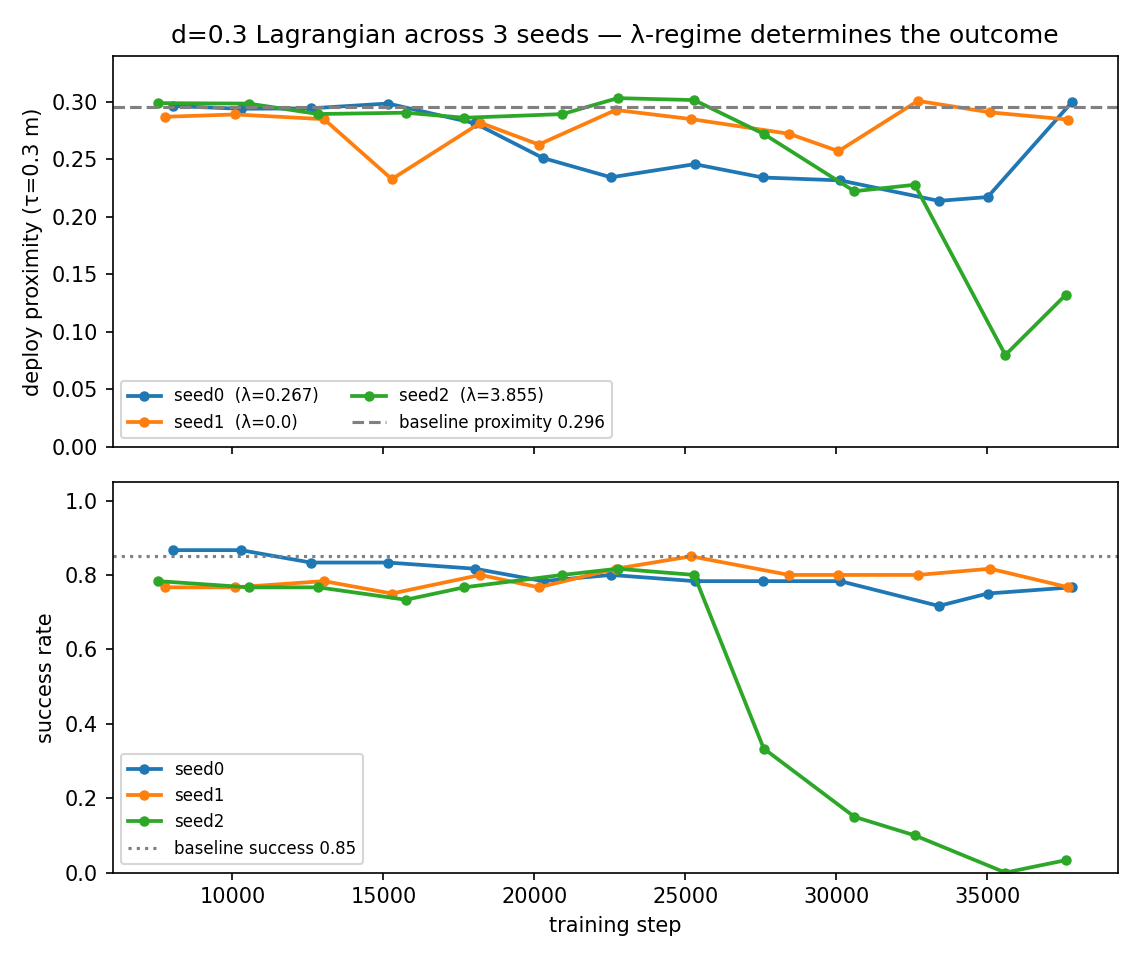
\includegraphics[width=0.55\textwidth]{d0p3_3seed_lambda_regimes.png}
\caption{The budget-feasibility experiment (E3.2; RQ1).
PID-Lagrangian at the only feasible
budget $d = 0.3$, three seeds. Top: deployment proximity-violation
rate ($\tau = 0.3$\,m) versus training step; bottom: task success. The
seeds converge to $\lambda = 0.000$ (seed~1, unconstrained, flat at
the baseline $\approx$0.30), $\lambda = 0.267$ (seed~0, a graceful
sub-0.26 avoidance basin), and $\lambda = 3.855$ (seed~2, windup
collapse, success $\to 0$). Because $d = 0.3$ coincides with the
task's inherent cost, the dual variable carries too little signal to
auto-tune stably, motivating the fixed-$\lambda$ headline.}
\label{fig:lambda-regimes}
\end{figure}

\subsection{The Reactive-Filter Pareto Frontier}
\label{sec:results:filter-pareto}

The offline SVF was trained at $\alpha_{\mathrm{CQL}} = 5.0$ and
swept over the veto threshold $R$ on a held-out validation set (three
seeds, 20 episodes each). With the filter disabled ($R = 0$) the
swept \texttt{ep\_proximity\_violation\_rate} is $0.286$, which
matches the unconstrained benchmark baseline of $0.296$ to within
sampling error; this agreement is the validation check that the
sweep environment reproduces the deployment environment.

The sweep does \emph{not} expose an operating point that reduces the
proximity-violation rate cheaply: $R = 2.25$ cuts the rate by only
$\approx$8\,\% at $\approx$15\,\% intervention, a one-third
reduction needs $\approx$67\,\% intervention, and even vetoing
\emph{every} step caps the reduction at $\approx$58\,\%, the
decomposition of Section~\ref{sec:exogenous} seen from the filter
side. We therefore pin the operating point at the light backstop
$R = 2.25$ and read the veto as an \iso{}~\ssm{} velocity backstop,
not a proximity-violation-rate reducer; proactive exposure reduction is delegated
to the constrained policy
(Section~\ref{sec:results:headline-feature-table}).

\paragraph{The reactive-fallback dilemma.}
A natural objection is that a more aggressive fallback would let the
filter reduce the proximity-violation rate directly. A fallback sweep on the
unconstrained baseline at matched intervention rates rules this out.
Zero-velocity braking holds station: it trims mean robot speed (the
velocity-backstop effect) but leaves the proximity-violation rate unchanged
($0.296 \to 0.303$), because the robot simply dwells while the human
approaches. An aggressive retreat cuts the proximity-violation rate sharply
($0.296 \to 0.095$) but only by having the robot flee: success
collapses from $0.85$ to $0.18$, mean speed rises sixfold
($0.29 \to 1.70$\,m/s), and the \ssm{}-actual rate \emph{worsens}
($0.147 \to 0.180$) because a fast-retreating robot is itself an
\ssm{} hazard. A gentle retreat does neither job. No reactive
setting buys geometric separation at acceptable success and speed:
against an approaching human, reducing the proximity-violation rate requires sustained,
anticipatory robot motion, which a one-step reactive filter cannot
supply. The veto remains independently useful as a deployment
backstop that trims mean speed without any retraining, but the
graded margin \iso{} prescribes needs the speed-scaling filter
(Section~\ref{sec:results:reactive-taxonomy}). This is the empirical
case for assigning the exposure axis to the policy part, revisited in
Section~\ref{sec:disc:filter-role}.

\subsection{The Headline Comparison: A Division of Labour}
\label{sec:results:headline-feature-table}

\textbf{Main comparison.} The central question is which mechanism
reduces which \iso{} axis, and how the mechanisms compose. The answer
is a \emph{division of labour}. The proactive constrained-RL policy
owns the exposure axis. A complementary runtime filter owns
the velocity (\ssm{}-actual) axis.
Table~\ref{tab:e4.1-feature-incremental} reports the four
configurations that establish this. The two reactive-veto
configurations are covered in
Section~\ref{sec:results:reactive-taxonomy}. The both-axis composition
is analysed in Section~\ref{sec:results:joint-coverage}.

\paragraph{The proactive policy reduces the proximity-violation rate, reproducibly.}
The fixed-$\lambda$ ($\lambda = 0.1$) Lagrangian policy reduces
\texttt{ep\_proximity\_violation\_rate} from the baseline $0.296$ to
$0.228$. This is a $22.8\,\%$ reduction (95\,\% CI
$[0.194, 0.264]$) at $0.76$ task success (95\,\% CI $[0.70, 0.82]$), pooled
over three seeds and 180 episodes. Each seed's selected operating
point is below the baseline. The velocity-adaptive \ssm{}-actual rate
also improves ($0.146 \rightarrow 0.112$, $-23\,\%$), while mean robot
velocity rises only $\sim$8\,\%. This is the kind of graceful
proximity-violation reduction the reactive filter could not achieve
(Section~\ref{sec:results:filter-pareto}). The magnitude is bounded by
the $\approx$42\,\% exogenous floor (Section~\ref{sec:exogenous}). It
captures roughly $40\,\%$ of the \emph{reducible}, robot-driven
proximity-violation rate. The absolute change is modest, but the reactive filter
captured essentially none of this component at acceptable cost.

\begin{table}[htbp]
\centering
\caption{Experiment E4.1 (\textbf{the headline}). The division of
labour between the proactive policy and a complementary-axis runtime
filter on \texttt{saucepan\_to\_hob} under \texttt{coworker\_train},
\texttt{noisy} perception. Rows 1 and 3 evaluate the single stage-2
baseline policy over 60 episodes (3 evaluation seeds $\times$ 20);
rows 2 and 4 pool three independently trained seeds (180 episodes).
Brackets are 95\,\% bootstrap CIs. The policy owns the
exposure axis ($\tau = 0.3$\,m proximity-violation rate); the graded speed-scaling
filter owns the velocity-adaptive \ssm{}-actual axis; only their
composition reduces both at once, at a multiplicative success cost.
$\Delta$ columns are relative to the unconstrained baseline (negative
is safer). The two SVF-veto configurations are in
Table~\ref{tab:filter-taxonomy}.}
\label{tab:e4.1-feature-incremental}
\small
\setlength{\tabcolsep}{4pt}
\resizebox{\textwidth}{!}{%
\begin{tabular}{lcccccc}
\toprule
Configuration & \texttt{succ.} & prox.-viol.\ rate & $\Delta$ prox.-viol.\ & \texttt{ssm-act.} & $\Delta$ ssm.\ & Interv.\ \\
\midrule
Unconstrained baseline                 & $0.85$ & $0.296\,[0.23, 0.37]$ & --       & $0.146\,[0.10, 0.19]$ & --       & -- \\
Proactive policy ($\lambda{=}0.1$)     & $0.76$ & $\mathbf{0.228}\,[0.19, 0.26]$ & $\mathbf{-23\,\%}$ & $0.112\,[0.09, 0.13]$ & $-23\,\%$ & -- \\
Speed-scaling filter (on baseline)     & $0.53$ & $0.273\,[0.21, 0.35]$ & $-8\,\%$ & $\mathbf{0.048}\,[0.03, 0.07]$ & $\mathbf{-67\,\%}$ & $45\,\%$ \\
\textbf{Policy $+$ speed-scaling (composition)} & $\mathbf{0.44}$ & $0.250\,[0.21, 0.29]$ & $-15\,\%$ & $0.065\,[0.05, 0.08]$ & $-55\,\%$ & $40\,\%$ \\
\bottomrule
\end{tabular}%
}
\end{table}

\paragraph{Operating-point selection must be safety-aware.}
A methodological point underwrites the policy row. At the feasible
budget the avoidance does not live at the peak-success checkpoint:
\texttt{snapshot\_best} (peak success) and the final checkpoint both
deploy at approximately the baseline proximity-violation rate ($\approx$0.30), because
selecting on task success picks \emph{against} the cost constraint. The
avoidance lives in a mid-training basin ($\sim$20k--35k steps, several
consecutive checkpoints at $0.21$--$0.25$ with success $0.72$--$0.80$
and \ssm{}-actual improved). The operating point must therefore be
chosen by a \emph{safety-aware} rule (lowest deployment
proximity-violation rate at a
success floor), not by peak success; selecting on success produced two
false-null results before the basin was found. Each seed's selected
basin checkpoint is shown in Figure~\ref{fig:fixlam}; that the basin
appears consistently across all three seeds under fixed $\lambda$ is
what makes the reduction reproducible, in contrast to the PID
instability of Figure~\ref{fig:lambda-regimes}.

\paragraph{The basin is constraint-driven, not selection noise.}
Selecting a checkpoint by a deployment metric invites the objection
that the ``basin'' is evaluation noise harvested by the rule. Four
observations rule this out: the $\lambda = 0$ seed, processed by the
\emph{same} rule, shows no basin (flat at $\approx$0.30 with
isolated dips); the basin is a \emph{run} of consecutive checkpoints
at $0.21$--$0.26$ proximity-violation rate with success $0.72$--$0.80$
(Figure~\ref{fig:fixlam}), not a single dip; \ssm{}-actual
co-improves inside it, which uncorrelated proximity noise would not
produce; and the selected point also sits below the
\emph{no-shaping} baseline at matched success (the $-12\,\%$
comparison below). When $\lambda$ engages, the constraint does work;
when it is slack, no selection rule manufactures a basin.

\begin{figure}[htbp]
\centering
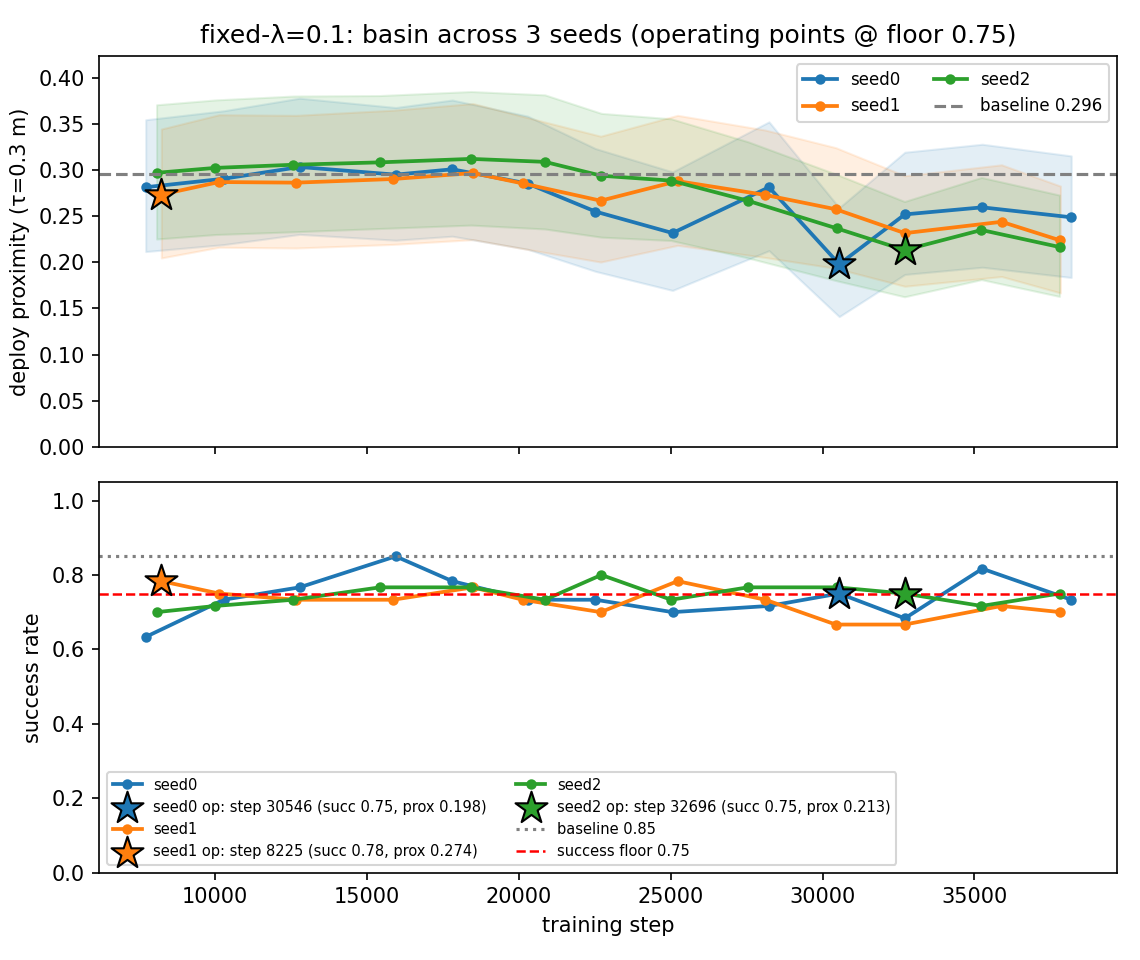
\includegraphics[width=0.55\textwidth]{fixlam0p1_3seed_floor075.png}
\caption{The fixed-$\lambda = 0.1$ policy across three seeds (stars
mark the safety-aware operating point at a success floor of $0.75$).
Top: deployment proximity-violation rate; bottom: success. Unlike the
PID runs (Figure~\ref{fig:lambda-regimes}), all three seeds behave
consistently and each reaches a sub-baseline proximity-violation-rate basin in
mid-training, giving the pooled $0.228$ at $0.76$ success. Fixing
$\lambda$ removes the ill-conditioned budget loop that made the PID
controller seed-unstable.}
\label{fig:fixlam}
\end{figure}

Appendix~\ref{app:walk-lagrangian}
(Figure~\ref{fig:lagrangian-vs-baseline}) shows the two behaviours
frame by frame: the baseline working through the coworker's reach
window in repeated proximity violation, and the constrained policy
yielding away and returning once the coworker departs.

\paragraph{Controlling for the workspace-shaping confound.}
The unconstrained baseline carries a mild workspace-distance reward
($\beta = 0.05$, Section~\ref{sec:bench:workspace}) that anchors the
end-effector in the task workspace. A natural objection is that this
inflates the baseline's proximity-violation rate and hence the constrained policy's apparent
reduction. Ablating it: the no-shaping baseline is $0.75$ success /
$0.258$ proximity-violation rate, versus the shaping baseline's $0.85$ / $0.296$. So
shaping is a \emph{task-success aid that incidentally raises
proximity-violation rate} (it keeps the robot where the coworker reaches), not a
safety term. Crucially, the Lagrangian policy ($0.228$ at $0.76$) sits
below the no-shaping baseline too, a $-12\,\%$ proximity-violation
rate reduction at
matched success, so the headline $-23\,\%$ (against the matched-recipe
baseline) is not an artefact of an inflated reference. We report both:
$-23\,\%$ (isolated constraint effect, shaping held fixed) and
$-12\,\%$ (confound-controlled, against the vanilla baseline).

\paragraph{The velocity axis is the filter's, and only a graded filter
reaches it.}
A runtime filter's canonical \iso{} role is the velocity axis. The
graded speed-scaling filter delivers it: on the baseline it drives
\ssm{}-actual from $0.146$ to $0.048$ ($-67\,\%$) at its optimum
($d_{\mathrm{slow}} = 0.40$\,m), with proximity-violation rate essentially unchanged
($0.296 \rightarrow 0.273$). It is the only filter in the taxonomy
that meaningfully reduces \emph{any} \iso{} axis on its own terms;
the binary veto, despite also slowing the robot, leaves
\ssm{}-actual at $0.148 \approx$ baseline, a stop-or-go veto does not
maintain the graded margin the standard prescribes. The success
cost, however, is not an artefact of the $0.40$\,m setting: even the
gentlest swept point ($d_{\mathrm{slow}} = 0.25$\,m) intervenes on
$37\,\%$ of steps, co-location is persistent, so some part of the
robot is nearly always inside the slow radius, and still costs a
third of task success at \emph{less} velocity-axis gain. The
reactive cost is paid at every operating point; only its exchange
rate moves.

\paragraph{The composition is the only both-axis-compliant
configuration, and it costs success.}
Composing the policy with the speed-scaling filter is the \emph{only}
configuration that reduces both \iso{} axes at once: geometric
proximity-violation rate $0.250$ (retained from the policy's $0.228$, CIs overlap)
\emph{and} \ssm{}-actual $0.065$ ($-42\,\%$ against the policy's
$0.112$, the filter's contribution). Each component alone leaves the
\emph{other} axis near baseline (policy: \ssm{}-actual $0.112$;
filter-alone: proximity-violation rate $0.273 \approx$ baseline). The cost is task
success: $0.85 \rightarrow 0.44$. The proactive cost ($0.85 \to 0.76$,
$\times 0.89$) and the reactive cost ($\times 0.58$) stack
\emph{multiplicatively}, and the composition beats neither specialist
on that specialist's own axis (the policy still wins proximity-violation rate
$0.228 < 0.250$; the filter still wins velocity $0.048 < 0.065$). The
composition is the joint-coverage compromise, not a per-axis champion.
Both measured safety axes are improved in this regime only by composing
the proactive policy with a complementary runtime filter, and that
composition makes the safety--throughput trade explicit, with a cost
dial tunable through $\lambda$ and $d_{\mathrm{slow}}$
(Section~\ref{sec:results:joint-coverage}).

\paragraph{Sim-to-real perception.}
The whole table is evaluated under \texttt{bodyslam=noisy}, the
realistic deployment condition and the filter's native distribution
(Section~\ref{sec:setup:perception-mode}). The constrained policy's reduction
survives this noisy, lagged perception unchanged (E3.6,
Section~\ref{sec:results:obs-rl}): the architecture claim is reported
under deployment-relevant perception, not only under oracle state.

\subsection{The Reactive-Filter Taxonomy: Freeze versus Flee}
\label{sec:results:reactive-taxonomy}

The headline filter is the graded speed-scaling one. The architecture
was originally built around a learned \textsc{CQL} safety value
function used as a veto, so that design is evaluated too. We tested
every reactive modality available, learned and model-based. None
reaches the proactive policy's graceful operating point. The reason is
structural. A reactive filter acts only \emph{once the human is already
close}. At that point the robot can either \emph{freeze} and dwell in
the danger zone, or \emph{flee} and abandon the task.
Table~\ref{tab:filter-taxonomy} summarises the taxonomy;
Appendix~\ref{app:walk-veto} (Figure~\ref{fig:svf-veto-anatomy})
illustrates one veto event frame by frame — the safe/unsafe
classification, both fallbacks branched from the same vetoed state, and
the no-filter counterfactual. The claim is
scoped carefully: \emph{no reactive filter gracefully reduces the
proximity-violation rate under persistent co-location}. It is a
statement about the exposure axis in this regime, not about reactive
filtering in general.
Section~\ref{sec:results:r2} shows what reactive mechanisms can
deliver on the velocity axis when co-location is intermittent and
genuinely-safe windows exist.

\begin{table}[htbp]
\centering
\caption{The reactive-filter taxonomy on \texttt{saucepan\_to\_hob}
(\coworker{}, \texttt{noisy}); every row is 60 evaluation episodes,
and rows involving the constrained policy use the seed-0 trained
policy (the pooled three-trained-seed policy numbers are in
Table~\ref{tab:e4.1-feature-incremental}). Every reactive modality,
learned or model-based, is bounded by the freeze-versus-flee dilemma:
it either freezes (and the proximity-violation rate does not fall) or
flees (and task success collapses). None reaches the proactive policy's
frontier (success $0.75$, proximity-violation rate $0.198$ at seed~0;
$0.76$/$0.228$ pooled).
The SVF veto applied to the \emph{policy} (the architecture's
original composition design) is worse than the policy alone.}
\label{tab:filter-taxonomy}
\small
\begin{tabular}{llccc}
\toprule
Filter & Mechanism & Prox.\ viol.\ rate & Success & Interv.\ \\
\midrule
Learned veto (SVF), on baseline   & velocity backstop (freeze) & $0.303$ & $0.78$ & $15\,\%$ \\
Learned veto (SVF), on policy     & freeze $\to$ dwell         & $0.265$ & $0.62$ & $48\,\%$ \\
Model-based base-dodge (CBF)      & flee (retreat base)        & $0.150$ & $0.57$ & $1.3\,\%$ \\
Model-based EE-retract (CBF)      & flee (retract arm)         & $0.155$ & $0.50$ & $5.8\,\%$ \\
\textbf{Proactive policy ($\lambda{=}0.1$)} & \textbf{anticipatory avoid} & $\mathbf{0.198}$ & $\mathbf{0.75}$ & -- \\
\bottomrule
\end{tabular}
\end{table}

\paragraph{The learned veto freezes.}
On the baseline, the SVF veto with a zero-velocity fallback
($R = 2.25$, $15\,\%$ intervention) does not reduce the proximity-violation rate
($0.296 \rightarrow 0.303$, within noise); it only trims mean robot
velocity ($-8\,\%$), acting as an \ssm{} \emph{velocity backstop}
(Section~\ref{sec:results:filter-pareto}). Applied on top of the
already-avoiding policy, it is \emph{counterproductive}: the proximity-violation rate
worsens ($0.198 \rightarrow 0.265$) and success falls
($0.75 \rightarrow 0.62$), at a $48\,\%$ intervention rate (versus
$15\,\%$ on the baseline). The mechanism is distribution shift: the SVF
critic was collected on \emph{baseline} rollouts, so it is out of
distribution on the avoiding policy and over-vetoes, and each veto
zeroes robot velocity, re-introducing the freeze/dwell failure. A
threshold sweep confirms this is not mis-thresholding, $R \in [1.0,
2.25]$ gives $39$--$48\,\%$ intervention and proximity-violation rate $0.27$--$0.28$ at
every setting, and re-collecting the critic on the policy's own
rollouts (on-policy) still yields no graceful operating point: at
$\le 25\,\%$ intervention every threshold \emph{increases} the
proximity-violation rate, and the rate falls only at $65$--$100\,\%$
intervention where the robot
is essentially frozen. Neither critic meets the pre-registered
gracefulness bar ($\geq 30\,\%$ proximity-violation reduction at $\leq 25\,\%$
intervention, Section~\ref{sec:setup:metrics}). Both the
baseline-trained and on-policy critics fail at every threshold, so the
limit is the reactive paradigm, not the critic's calibration.

\paragraph{The model-based filter flees.}
A geometric control-barrier-style ``directional-dodge'' filter (no
learned critic) \emph{does} reduce the proximity-violation rate where the veto cannot,
$0.198 \rightarrow 0.150$ at $d_{\mathrm{target}} = 0.35$\,m and only
$1.3\,\%$ intervention, but by \emph{fleeing}: the base retreats,
episodes stretch from $\sim$450 to $620$--$770$ steps, and success
falls to $0.57/0.43/0.35$ as $d_{\mathrm{target}} = 0.35/0.45/0.55$,
with the proximity-violation rate flooring at $\approx$0.14 regardless (the exogenous
floor). There is no harmless-backstop setting: even at the minimal
$d_{\mathrm{target}} = 0.30$\,m ($1.1\,\%$ intervention) success
falls $0.75 \rightarrow 0.58$, because even rare dodges land at
task-critical moments. The same flee appears whichever part of the
robot dodges: retracting the \emph{end-effector} (an arm ``flinch''
via a damped-Jacobian step) is worse in the useful regime ($0.50$
success at $d = 0.35$; the EE is the closest pair, so it intervenes
far more often, and retracting the arm \emph{is} pausing the task).
The flee is structural: the task and the hazard are co-located, so a
separation barrier is satisfiable only by radial retreat, which is
retreat from the workspace. Eliminating the flee requires
anticipation, which is exactly what the constrained policy provides;
``fixing'' the flee inside a reactive filter amounts to reinventing
the policy.

\subsection{Joint ISO Coverage: The Composition and Its Ceiling}
\label{sec:results:joint-coverage}

The two preceding subsections separate cleanly onto the two \iso{} axes
(Figure~\ref{fig:axis-division}). Figure~\ref{fig:velocity-axis} makes
the velocity axis explicit. On \ssm{}-actual, the speed-scaling filter
is the specialist ($\rightarrow 0.048$). The policy also helps through
avoidance ($\rightarrow 0.112$), because keeping further from the human
lowers the required margin. The SVF veto does not help
($0.148 \approx$ baseline). Figure~\ref{fig:joint-coverage} plots both
axes together. Only the policy-plus-speed-scaling composition reaches
the both-safe corner: low proximity and low \ssm{}-actual. It is also
strictly better than the SVF-veto composition, which degrades proximity
with no velocity gain. A complementary, model-based filter composes
additively. A redundant, out-of-distribution learned filter does not.

The composition's success cost ($0.85 \to 0.44$, analysed in
Section~\ref{sec:results:headline-feature-table}) should be read as
\emph{the persistent-co-location regime's ceiling}, not as a defect of
the composition: when the coworker is co-located most of the time,
any separation-triggered speed response is active most of the time
(measured directly in Section~\ref{sec:results:boundary}), so the
reactive cost is paid almost everywhere and stacks with the
proactive cost. Under this regime, both-axis \iso{} safety is
purchasable only at stacked cost; whether a smarter trigger
(a learned critic gating the scaler) can avoid that cost is exactly
the question the intermittent-co-location chapter answers in the
affirmative, and Section~\ref{sec:results:boundary} answers in the
negative \emph{for this regime}.
Appendix~\ref{app:walk-speedscale}
(Figure~\ref{fig:speedscale-mechanism}) shows the scaling law acting
frame by frame: full speed while the coworker is clear, a graded
slow-down as separation closes.

\begin{figure}[htbp]
\centering
\begin{subfigure}[t]{0.48\textwidth}
  \centering
  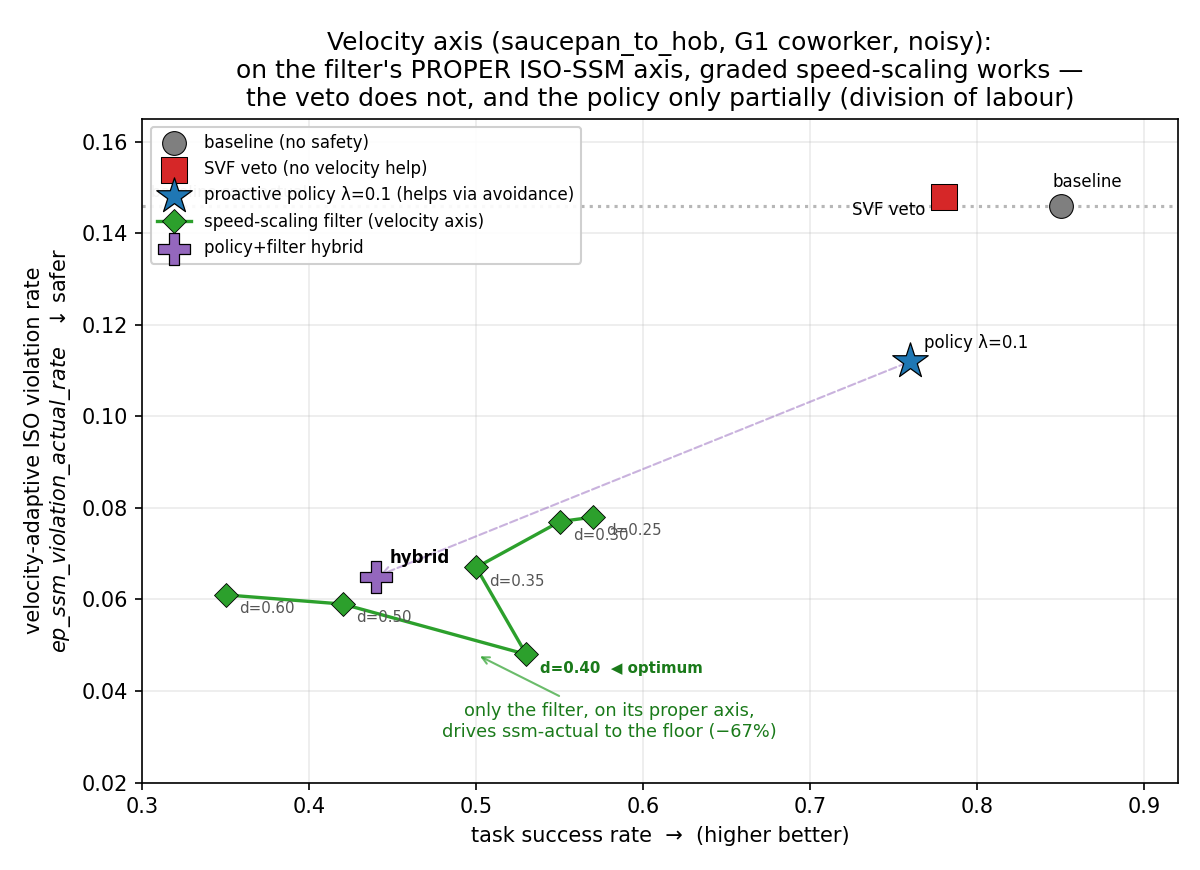
\includegraphics[width=\linewidth]{velocity_axis.png}
  \caption{The velocity (\ssm{}-actual) axis: the graded
  speed-scaling filter is the specialist; the policy also reduces it
  via avoidance; the veto does not maintain the graded margin and
  leaves it at baseline.}
  \label{fig:velocity-axis}
\end{subfigure}\hfill
\begin{subfigure}[t]{0.48\textwidth}
  \centering
  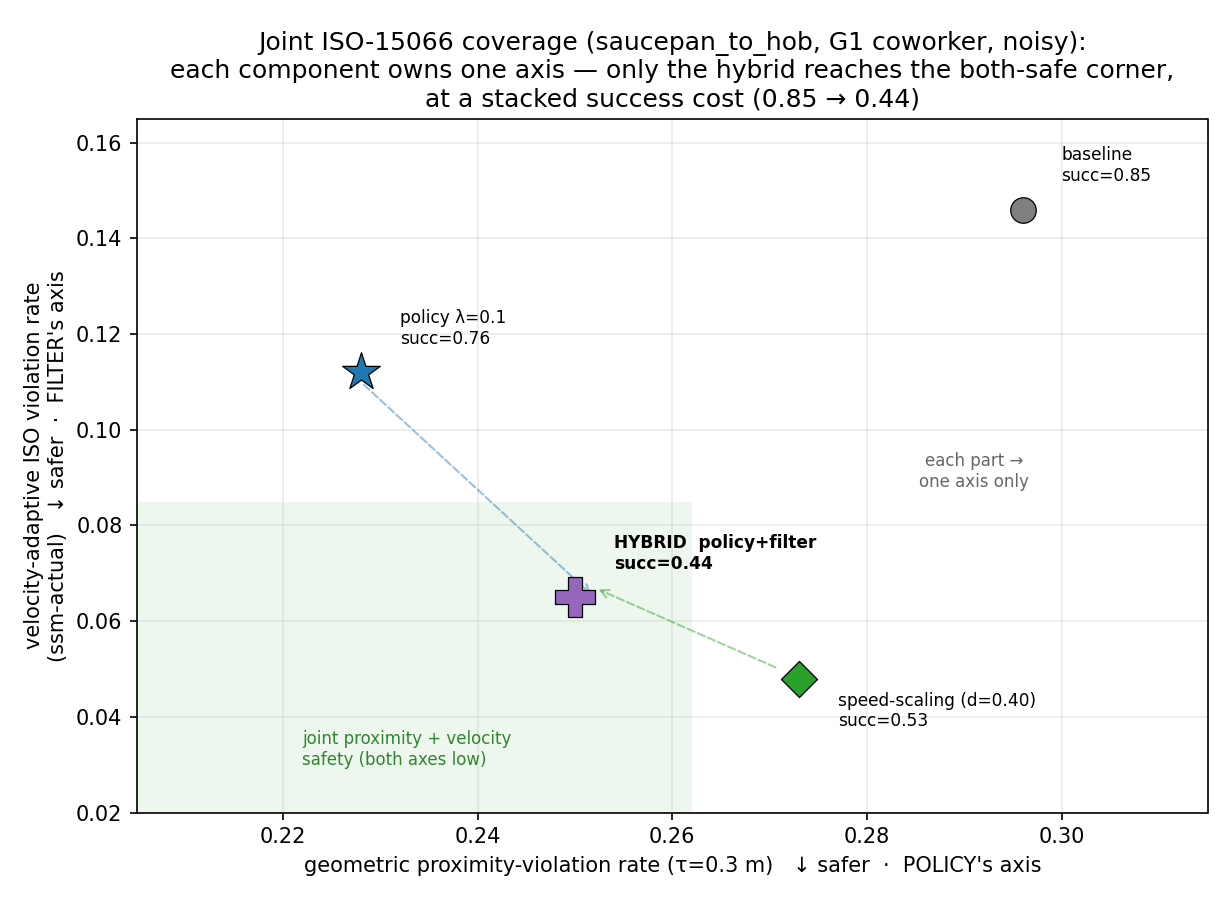
\includegraphics[width=\linewidth]{joint_coverage.png}
  \caption{Joint coverage: proximity-violation rate ($x$, policy's axis) vs.\
  \ssm{}-actual ($y$, filter's axis). Only the composition reaches
  the both-safe corner, at success $0.44$; it beats neither
  specialist on that specialist's own axis.}
  \label{fig:joint-coverage}
\end{subfigure}
\caption{The two-axis division of labour on
\texttt{saucepan\_to\_hob} (60-episode cells, \texttt{noisy}
perception, \coworker{} distribution) and what composing the
specialists buys. The policy owns the proximity-violation axis, the graded
speed-scaling filter owns the velocity axis, and only their
composition reaches the corner where both \iso{} axes improve at
once, at a success cost ($0.85 \to 0.44$) that
Section~\ref{sec:results:boundary} shows to be the persistent
regime's ceiling rather than a tuning defect.}
\label{fig:axis-division}
\end{figure}

\subsection{The Policy Does Not Internalise the Filter}
\label{sec:results:interaction}

If the policy and the SVF veto were complementary in the originally
hypothesised sense, the filter's required intervention rate would
\emph{fall} as the Lagrangian policy is trained, the policy
progressively taking over the filter's job. E4.3 evaluates the SVF
veto's intervention rate on intermediate snapshots of the
fixed-$\lambda$ policy across training. It does \emph{not} fall: it
stays at $\sim$40--60\,\% throughout (mean $\sim$49\,\%, Figure~\ref{fig:e4.3-internalisation}),
\emph{higher} than the $\sim$15\,\% intervention on the unconstrained
baseline, not lower. The reason is the distribution shift of
Section~\ref{sec:results:reactive-taxonomy}: the constrained policy's
state--action distribution is precisely where the baseline-collected
critic is least calibrated, so as the policy avoids \emph{more}, the
critic vetoes \emph{more}. This is the corroborating mechanism behind
the counterproductive veto composition: there is no internalisation
curve to report because the baseline-calibrated filter never becomes
redundant in the benign direction; it becomes \emph{more} active and
counterproductive.

\begin{figure}[htbp]
\centering
\begin{tikzpicture}
\begin{axis}[
  width=0.66\textwidth, height=0.36\textwidth,
  xlabel={Lagrangian training step},
  ylabel={SVF-veto intervention rate},
  xmin=0, xmax=40000, ymin=0, ymax=0.65,
  scaled x ticks=false, xtick={0,10000,20000,30000,40000},
  xticklabels={0,10k,20k,30k,40k},
  grid=both, grid style={black!10},
  tick label style={font=\footnotesize}, label style={font=\small},
  legend style={font=\footnotesize, at={(0.97,0.30)}, anchor=north east, draw=black!20},
]
\addplot[blue!70, thick, mark=*, mark size=1pt] coordinates {
  (2940,0.492)(5169,0.513)(7711,0.607)(10278,0.529)(12780,0.535)(15942,0.454)(17805,0.393)(20285,0.488)(22521,0.449)(25058,0.491)(28234,0.528)(30546,0.414)(32706,0.506)(35257,0.460)(38185,0.575)
};
\addlegendentry{SVF veto on constrained policy ($\lambda{=}0.1$, seed 0)}
\addplot[red!60, dashed, thick, no marks] coordinates {(0,0.15)(40000,0.15)};
\addlegendentry{SVF veto on unconstrained baseline}
\end{axis}
\end{tikzpicture}
\caption{Experiment E4.3. The SVF veto's intervention rate on the
constrained policy does \emph{not} fall during training; it stays at
$\sim$40--60\,\% (blue), above the $\sim$15\,\% it requires on the
unconstrained baseline (red dashed). A complementary filter would show
a falling curve; this flat, elevated curve is direct evidence that the
baseline-collected critic is out of distribution on the avoiding
policy and over-vetoes, the mechanism behind the counterproductive
SVF-veto composition
(Section~\ref{sec:results:reactive-taxonomy}).}
\label{fig:e4.3-internalisation}
\end{figure}

The deployment implication inverts the originally intended one: a
filter intended to compose with a learned policy must either be
collected on that policy's rollouts (still insufficient here,
Section~\ref{sec:results:reactive-taxonomy}) or operate on an axis
the policy does not move along, which is exactly why the graded
speed-scaling filter, on the velocity axis, composes where the veto
does not.

\subsection{The Avoidance Survives Realistic Perception}
\label{sec:results:obs-rl}

To test whether the learned avoidance depends on perfect state
estimation, we re-evaluated the \emph{same} fixed-$\lambda$ constrained policy
(fixed-$\lambda$, Section~\ref{sec:results:headline-feature-table})
under two perception regimes: \texttt{oracle} (ground-truth human
pose) and \texttt{noisy} (the calibrated mock-\bodyslampp{} estimate
with measurement noise and a 3-step latency). The avoidance is
\emph{not} perception-bottlenecked: the proximity-violation rate is
statistically indistinguishable across regimes ($0.236$ oracle vs.\
$0.198$ noisy), both far below the unconstrained baseline's
$\approx$0.30, and task success is comparable ($0.82$ vs.\ $0.75$).
The baseline, by contrast, shows \emph{no} oracle--noisy gap ($0.302$
vs.\ $0.296$): it does not use the human channel to avoid, so
perception quality cannot help it. The fixed-$\lambda$ constrained
policy keeps its proximity-violation-rate reduction under noisy, lagged
perception. This suggests that the avoidance behaviour is robust, not
an artefact of perfect simulator state (Table~\ref{tab:e3.6-obs-rl}).

\begin{table}[htbp]
\centering
\caption{Experiment E3.6. The constrained policy (seed-0 trained)
and the unconstrained baseline re-evaluated under \texttt{oracle} and
\texttt{noisy} perception (\texttt{saucepan\_to\_hob},
\texttt{coworker\_train}; each cell is 60 episodes, 3 evaluation
seeds $\times$ 20). The constrained policy's proximity-violation-rate reduction is preserved
under realistic noisy, lagged perception (bootstrap CIs across modes
overlap: $0.236\,[0.17, 0.30]$ oracle vs.\ $0.198\,[0.14, 0.26]$
noisy), and the baseline shows no oracle--noisy gap because it does
not use the channel to avoid. The headline E4.1 table reports the
pooled three-trained-seed \texttt{noisy} numbers.}
\label{tab:e3.6-obs-rl}
\small
\begin{tabular}{lcccc}
\toprule
 & \multicolumn{2}{c}{Unconstrained baseline} & \multicolumn{2}{c}{Constrained policy ($\lambda{=}0.1$)} \\
\cmidrule(lr){2-3}\cmidrule(lr){4-5}
Perception & \texttt{succ.} & prox.-viol.\ rate & \texttt{succ.} & prox.-viol.\ rate \\
\midrule
\texttt{oracle} & $0.77$ & $0.302$ & $0.82$ & $0.236$ \\
\texttt{noisy}  & $0.85$ & $0.296$ & $0.75$ & $0.198$ \\
\bottomrule
\end{tabular}
\end{table}

A third, ``perception-off'' mode is architecturally inapplicable
(removing the channel changes the input size, $288 \to 264$, so the
trained weights cannot run); a genuine no-human-observation
condition is the separately trained behaviour-cloning ablation
(Section~\ref{sec:results:obs-bc}). The perception sweep is thus a
two-mode comparison by construction.

\subsection{The Worst-Case Tail Is Exogenous and Uncontrollable}
\label{sec:results:tail}

\iso{} compliance is a worst-case rather than an average property, so
the tail of the per-episode separation distribution is the
safety-relevant quantity. The central tail finding is that the policy
lowers the \emph{mean} and \emph{frequency} of proximity but
\emph{not} the worst-case tail. Mean separation improves modestly
(baseline $0.132$\,m $\rightarrow$ policy $0.140$\,m), but the
worst-5\,\% closest approach is essentially unchanged across the
unconstrained baseline, the no-shaping baseline, and the constrained
policy alike: $\cvar_{0.95}$ of \texttt{ep\_min\_separation}
$\approx 0.005$\,m and the single worst approach
$\approx 0.002$\,m in every configuration
(Table~\ref{tab:e5.1-tail}).

This does not mean that the whole exogenous tail is necessarily an
injury-level violation. It is a closest-distance tail. If the robot is
stationary, some close approaches may remain benign under \pfl{} if
contact forces stay below biomechanical limits. The current report
cannot test that distinction because reliable human--robot contact
forces are not available (Section~\ref{sec:disc:pfl-bug}).

\begin{table}[htbp]
\centering
\caption{Experiment E5.1. Separation statistics across the headline
configurations (\coworker{}, \texttt{noisy}). The policy improves the
\emph{mean} separation but the worst-case tail ($\cvar_{0.95}$ and the
single worst approach) is unchanged, because the closest approach is
the coworker's lunge toward a robot it is co-located with, an
\emph{exogenous} event no robot-action policy or filter can remove.
The controllable quantity is the dwell and frequency of proximity violations, not
the single worst-case approach. The table reports distance tails, not
\pfl{} force violations.}
\label{tab:e5.1-tail}
\small
\begin{tabular}{lccc}
\toprule
Configuration & mean sep.\ (m) & $\cvar_{0.95}$ min-sep (m) & worst min-sep (m) \\
\midrule
Unconstrained baseline             & $0.132$ & $\approx 0.005$ & $\approx 0.002$ \\
Proactive policy ($\lambda{=}0.1$) & $0.140$ & $\approx 0.005$ & $\approx 0.002$ \\
\bottomrule
\end{tabular}
\end{table}

This is the exogenous decomposition of
Section~\ref{sec:exogenous} seen from its tail end:
$\approx$58\,\% of proximity-violation time is robot-driven (suppressible by
avoidance) and $\approx$42\,\% is human-driven, and the worst single
approach lives entirely in the human-driven remainder. The policy
captures roughly $40\,\%$ of the reducible part; no robot-side
mechanism, and no configuration evaluated anywhere in this report,
policy, veto, dodge, speed-scaling, or composition, moves
$\cvar_{0.95}$ of the closest approach. Honest reporting of this
floor is what makes the $-22.8\,\%$ headline a real, bounded number
rather than an over-claim, and it motivates the
Power-and-Force-Limiting collision-brake future work
(Section~\ref{sec:fw:pfl}), the only mechanism class that could
address the exogenous near-contact tail.

\subsection{Generalisation to a Held-Out Coworker Distribution}
\label{sec:results:ood}

Re-evaluating on a held-out coworker distribution (E5.2;
\texttt{coworker\_eval}: broader and gentler, closest
$0.6$--$1.8$\,m, reach $3$--$9$\,s, walk $0.6$--$2.2$\,m/s) tests
whether the fixed-$\lambda$ constrained policy's reduction is specific to the training coworker.
It is not: the reduction \emph{generalises}, and is proportionally
larger on the gentler distribution. The absolute proximity is much
lower there because the gentler coworker approaches less, but the
policy still cuts it by $31\,\%$ ($0.084 \rightarrow 0.058$, against
the in-distribution $0.296 \rightarrow 0.228$). The success cost is
\emph{larger} ($0.92 \rightarrow 0.70$) because $\lambda = 0.1$ was
tuned for the harder training coworker and over-constrains the
gentler one: the operating point is task- and distribution-specific,
but the qualitative result holds out of distribution. The SVF-veto
composition is again worse than the policy alone here ($54\,\%$
intervention), consistent with the in-distribution finding.

A third generalisation axis, \emph{cross-task} transfer of the full
pipeline (base curriculum $\rightarrow$ Lagrangian $\rightarrow$
eval) to \texttt{dishwasher\_close} and \texttt{drawers\_open\_all}
(E5.3), resolved \emph{negative}: the \texttt{saucepan\_to\_hob}
recipe does not replicate there, no budget binds usefully, and the best constrained
operating point is a marginal, within-noise improvement
(Section~\ref{sec:results:r2-lagrangian}). The word
``reproducibly'' in this chapter's headline therefore means
\emph{across the three \texttt{saucepan\_to\_hob} training seeds}, not across tasks.
The cross-task story is the regime map of
Section~\ref{sec:results:boundary}, and the failure of this transfer
is one side of the regime map rather than an unexplained null.

\section{Intermittent Co-location: Gate the Runtime Backstop}
\label{sec:results:r2}

This section covers the other side of the regime map. The coworker
distribution is unchanged (\coworker{}, \texttt{noisy}, 3 evaluation
seeds $\times$ 20 episodes per cell), but the close encounters arrive
in bursts. The co-location measurement of
Section~\ref{sec:results:boundary} puts a separation-triggered gate's
activity at $19$--$27\,\%$ of steps, compared with $51$--$63\,\%$ on
\texttt{saucepan\_to\_hob}. The claim is the regime map's second half: \emph{where close
encounters are separated by genuinely-safe windows, constrained RL has
nothing useful to bind on, and a learned critic gating a graded
speed-scaling backstop halves \ssm{} violations at a fraction of the
unconditional filter's success cost}. The persistent-regime recipe
fails in both directions. The fixed-$\lambda$ constrained policy that
reduced exposure on \texttt{saucepan\_to\_hob} finds no feasible budget
here (E3.3). The
runtime-filter family that was only a backstop there becomes, once
gated by the learned critic, the best safety--throughput operating
point in the evaluation (E2.6). This section works through that
reversal mechanism by mechanism.

\subsection{Constrained RL Finds No Feasible Budget (WCSAC Corroborates)}
\label{sec:results:r2-lagrangian}

The first budget sweep on these tasks bracketed the policies' natural
rolling cost ($\approx$0.25 on the \ssm{}-margin cost signal) from
above, with budgets $d \in \{0.1, 0.3, 0.5\}$: budgets above the
natural cost left $\lambda = 0$ (constraint inert, baseline
behaviour), and $d = 0.1$ drove $\lambda \to 21.5$ and $0\,\%$
success (task-fatal). E3.3 re-targets the budget \emph{into} the
unsampled window just below the natural cost,
$d \in \{0.16, 0.19, 0.22\}$ on both tasks, to test whether a
binding-but-feasible operating point exists at all
(Table~\ref{tab:e3.3-budget-sweep}).

\begin{table}[htbp]
\centering
\small
\caption{Experiment E3.3. Cost-budget retarget sweep on the
intermittent-co-location tasks (40k frames, single training seed per
cell, warm-started from the stage-2 curriculum snapshot; cost is the
graded \ssm{}-margin signal). Re-targeting makes the constraint
\emph{bind} ($\lambda > 0$ everywhere), but the rolling cost floors
at $\approx$0.21--0.25, at or above every budget, so $\lambda$
integrates upward and the task collapses. There is no budget that
both binds and preserves the task; even the floor budget has no
\emph{stable} feasible point (\texttt{dishwasher\_close} $d{=}0.22$ was at $1.00$
success at 37k frames, $\lambda = 0.69$, and collapsed to $0.30$ by
40k as $\lambda$ reached $1.5$).}
\label{tab:e3.3-budget-sweep}
\begin{tabular}{llcccl}
\toprule
Task & Budget $d$ & Final $\lambda$ & Rolling cost & In-train success & Outcome \\
\midrule
\texttt{dishwasher\_close} & 0.16 & 13.8 & 0.225 & 0.30 & binds hard, collapsed \\
\texttt{dishwasher\_close} & 0.19 & 9.3  & 0.235 & 0.10 & binds hard, collapsed \\
\texttt{dishwasher\_close} & 0.22 & 1.5  & 0.252 & 0.30 & binds late, collapsed \\
\texttt{drawers\_open\_all} & 0.16 & 10.4 & 0.209 & 0.00 & binds hard, collapsed \\
\texttt{drawers\_open\_all} & 0.19 & 5.2  & 0.231 & 0.30 & binds hard, collapsed \\
\texttt{drawers\_open\_all} & 0.22 & 1.3  & 0.236 & 0.60 & binds late, partial \\
\bottomrule
\end{tabular}
\end{table}

\paragraph{Deployment of the best cells confirms the cliff.}
Benchmarking each $d = 0.22$ cell's best $\lambda$-active basin
checkpoint and its final checkpoint under the deployment-faithful
harness (\texttt{noisy}, 60 episodes): on \texttt{dishwasher\_close} the basin
checkpoint is statistically the baseline (success $0.82\,[0.72,
0.92]$, proximity-violation rate $0.243\,[0.15, 0.34]$ vs.\ baseline $0.246$, a
$-1\,\%$ change), and the final checkpoint trades $-7\,\%$ proximity-violation rate
for success $0.48$. On \texttt{drawers\_open\_all} the single best feasible point in the
whole sweep, the $d = 0.22$ basin, reaches $-13\,\%$ proximity
violation rate ($0.211 \to 0.184\,[0.14, 0.24]$) at $-5$\,pt success, with a confidence interval that
overlaps the baseline: a marginal, within-noise improvement, not a
robust win. The relationship is a monotonic trade: the proximity-violation rate falls
only as success falls, with no graceful elbow anywhere in the swept
range.

\paragraph{When $\lambda$ binds, the robot gets \emph{faster}, not more careful.}
The mechanism of the collapse matters for what it rules out. Under a
binding multiplier the \texttt{dishwasher\_close} policy's mean velocity rises from
$0.44$ to $0.79$\,m/s and its max from $2.46$ to $4.14$\,m/s: the
cost pressure degrades action selection into fast, erratic motion
rather than producing careful slowing. A scalar penalty on
\emph{expected} cost evidently cannot, on these tasks, separate
task-necessary proximity from gratuitous risk; it can only destroy
the behaviour that incurs cost, which here is the task itself.

\paragraph{The trainability confound, stated honestly, and the external check.}
\label{sec:results:wcsac}
These are sparse-reward tasks on which the base policy is fragile
without the demonstration warm-start and curriculum, so ``constrained
RL fails here'' could in principle mean ``RL barely trains here.''
The WCSAC external baseline (E3.7, Section~\ref{sec:method:wcsac})
speaks to both readings at once (Table~\ref{tab:e3.7-wcsac}).
Trained from scratch, WCSAC \emph{learns \texttt{dishwasher\_close}} ($0.47$ success
at the tightest \cvar{} budget, proximity-violation $3.6\,\%$), so
the external reference is non-degenerate and the pipeline sound; but
it reaches $0\,\%$ on \texttt{drawers\_open\_all} at \emph{every} budget, corroborating
base-task fragility (its low violation numbers there are trivial: a
policy that never engages the task stays far from the human). The
verdict is therefore \emph{no feasible budget exists on these
tasks}, compounded by base-task fragility, not \emph{constrained RL
is universally ineffective}: the \texttt{saucepan\_to\_hob} policy of
Section~\ref{sec:results:r1} is the
counterexample, and the regime-level account of the flip is
taken up in Section~\ref{sec:results:boundary}.

\begin{table}[htbp]
\centering
\small
\caption{Experiment E3.7. WCSAC~\cite{yang2021wcsac} external
reference, reimplemented faithfully and trained from scratch (150k
frames, no demonstrations, single seed per cell; 30 evaluation
episodes, \texttt{oracle} human-state, so these are upper bounds with
respect to perception). WCSAC is non-degenerate on \texttt{dishwasher\_close} but
fails to learn \texttt{drawers\_open\_all} at any budget; the apparent budget ordering on
\texttt{dishwasher\_close} ($d{=}30$ at $0.03$) is within single-seed from-scratch
SAC variance and is not interpreted further. From-scratch WCSAC also
sits well below the demo-warm-started value-based Lagrangian
($0.47$ vs.\ $0.82$ peak on \texttt{dishwasher\_close}), quantifying how much of
task competence on these tasks comes from the demonstration prior.}
\label{tab:e3.7-wcsac}
\begin{tabular}{llcccc}
\toprule
Task & Budget & Final $\lambda$ & Success & Prox.\ viol. & Worst min-sep (m) \\
\midrule
\texttt{dishwasher\_close} & 5  & 100 (max) & 0.47 & 0.036 & 0.025 \\
\texttt{dishwasher\_close} & 15 & 4.5       & 0.43 & 0.102 & 0.009 \\
\texttt{dishwasher\_close} & 30 & 0         & 0.03 & 0.021 & 0.031 \\
\texttt{drawers\_open\_all} & 5  & 92        & 0.00 & 0.000 & 1.31 \\
\texttt{drawers\_open\_all} & 15 & 0         & 0.00 & 0.016 & 0.035 \\
\texttt{drawers\_open\_all} & 30 & 0         & 0.00 & 0.000 & 0.015 \\
\bottomrule
\end{tabular}
\end{table}

\subsection{A Binary Veto Breaks a Chunked Policy}
\label{sec:results:r2-veto}

The learned safety critic itself is sound here. The shared
\texttt{dishwasher\_close}/\texttt{drawers\_open\_all} SVF (Section~\ref{sec:method:filter}) separates safe
from unsafe transitions in-sample (mean $Q$ of $3.14$ on safe vs.\
$2.26$ on near-contact transitions; at $R = 2.75$ it catches
$92\,\%$ of near-contact transitions while vetoing $22\,\%$ of safe
ones). What fails is the \emph{intervention}: a binary veto that
zeroes velocity mid-chunk interacts destructively with the
temporal-ensemble action execution of the \cqnas{} policy
(Section~\ref{sec:impl:svf-faithful}). The robot stops inside a
blended action chunk, the ensemble's open-loop state runs ahead, and
when the veto lifts the policy fires a large catch-up action.
Max velocity \emph{rises}, $2.46 \to 3.77$\,m/s at $R = 2.25$ and to
$6.03$\,m/s at $R = 3.0$ (where the veto is active on $84\,\%$ of
steps and success has collapsed to $0.12$); the minimum \ssm{} margin
goes sharply negative ($0.16 \to -1.69$, $-6.84$); and the
\ssm{}-violation rate it was meant to reduce does \emph{not} improve
($0.176 \to 0.174$ on \texttt{dishwasher\_close}; $0.100 \to 0.130$, worse, on
\texttt{drawers\_open\_all}, where success falls $0.82 \to 0.43$). The override
\emph{form} is the design axis that matters
(Section~\ref{sec:bg:safe:recovery}): a hard switch is the wrong
intervention for chunked visuomotor policies, independent of how
good the critic that triggers it is.

\subsection{Unconditional Speed-Scaling Owns the Velocity Axis, at Heavy Cost}
\label{sec:results:r2-uncond}

Replacing the veto with the graded \iso{} speed-scaler
(Equation~\ref{eq:speed-scale}) removes the overshoot by
construction: it scales motion \emph{magnitude} while preserving the
policy's action direction, and max velocity is identical to the
baseline's ($2.46 \to 2.46$\,m/s). Applied unconditionally it is the first
mechanism in this entire research programme to substantially improve
the robot-controllable axis: \ssm{}-violation falls $0.176 \to 0.087$
($-50\,\%$) on \texttt{dishwasher\_close} and $0.100 \to 0.059$ ($-41\,\%$) on
\texttt{drawers\_open\_all}, with the minimum stopping margin improved on both. The cost
is indiscriminate: it slows the robot at \emph{every} close approach,
safe or not, and success falls $0.77 \to 0.52$ and $0.82 \to 0.38$.
That cost profile is exactly what a gate should fix, where the task
structure leaves the gate something to find.

\subsection{Critic-Gated Speed-Scaling: The When/How Split Recovers the Task}
\label{sec:results:r2-gated}

The critic-gated filter (Equation~\ref{eq:gated-rule}) assigns each
part of the decision to the component suited to it. The SVF decides
\emph{when} to intervene, firing only when
$Q_{\mathrm{safe}} < R$. The graded scaler decides \emph{how}, slowing
smoothly rather than vetoing. On these tasks, genuinely-safe windows
exist for the critic to find, so the split works
(Figure~\ref{fig:r2-method-comparison}, Table~\ref{tab:r2-methods}).
On \texttt{dishwasher\_close}, the gated filter at $R = 2.75$ retains the unconditional
scaler's full $-50\,\%$ \ssm{}-violation reduction at less than half
its success cost ($0.67$ vs.\ $0.52$, against a $0.77$ baseline). On
\texttt{drawers\_open\_all}, the recommended aggressive point
($R = 3.0$, $d_{\mathrm{slow}} = 0.8$) reaches $-22\,\%$ at $-0.09$
success. A near-free point ($R = 2.75$, $d_{\mathrm{slow}} = 0.8$)
gives $-10\,\%$ at $-0.02$ success. The gate-active fractions confirm
the mechanism. The gate fires on $27\,\%$ of steps on \texttt{dishwasher\_close} and
$19$--$27\,\%$ on \texttt{drawers\_open\_all}, depending on the threshold. Most steps
therefore pass at full speed.

\begin{table}[htbp]
\centering
\small
\caption{The intermittent-co-location method comparison (60 episodes
per cell, \texttt{noisy}, \coworker{}; both safety axes reported per
the two-axis protocol). $\Delta$ columns are relative to each task's
unconstrained baseline. The Lagrangian rows are the best basin
checkpoints from the seed-unstable budget sweep and carry that caveat
(Section~\ref{sec:results:r2-lagrangian}); WCSAC rows are the
external from-scratch reference at its best budget (single seed,
\texttt{oracle} perception). Only critic-gated speed-scaling reduces
the \ssm{}-velocity axis substantially while keeping success within
$0.10$ of baseline.}
\label{tab:r2-methods}
\setlength{\tabcolsep}{4pt}
\resizebox{\textwidth}{!}{%
\begin{tabular}{llccccc}
\toprule
Task & Method & Success & $\Delta$ succ. & \ssm{}-actual & $\Delta$ \ssm{} & Prox.\ viol. \\
\midrule
\texttt{dishwasher\_close} & Baseline (unconstrained)        & 0.77 & --      & 0.176 & --       & 0.246 \\
\texttt{dishwasher\_close} & Lagrangian (best basin, E3.3)   & 0.82 & $+0.05$ & 0.184 & $+5\,\%$ & 0.243 \\
\texttt{dishwasher\_close} & SVF veto ($R{=}2.25$)           & 0.63 & $-0.14$ & 0.174 & $-1\,\%$ & --    \\
\texttt{dishwasher\_close} & Speed-scale (unconditional)     & 0.52 & $-0.25$ & 0.087 & $-50\,\%$ & --   \\
\texttt{dishwasher\_close} & \textbf{Critic-gated ($R{=}2.75$)} & \textbf{0.67} & $\mathbf{-0.10}$ & \textbf{0.088} & $\mathbf{-50\,\%}$ & -- \\
\texttt{dishwasher\_close} & \emph{WCSAC (external, $d{=}5$)} & \emph{0.47} & \emph{$-0.30$} & -- & -- & \emph{0.036} \\
\midrule
\texttt{drawers\_open\_all} & Baseline (unconstrained)            & 0.82 & --      & 0.100 & --       & 0.211 \\
\texttt{drawers\_open\_all} & Lagrangian (best basin, E3.3)       & 0.77 & $-0.05$ & 0.082 & $-18\,\%$ & 0.184 \\
\texttt{drawers\_open\_all} & SVF veto ($R{=}2.25$)               & 0.43 & $-0.39$ & 0.130 & $+30\,\%$ & --   \\
\texttt{drawers\_open\_all} & Speed-scale (unconditional)         & 0.38 & $-0.44$ & 0.059 & $-41\,\%$ & --   \\
\texttt{drawers\_open\_all} & \textbf{Critic-gated ($R{=}3.0$, $d_{\mathrm{slow}}{=}0.8$)} & \textbf{0.73} & $\mathbf{-0.09}$ & \textbf{0.078} & $\mathbf{-22\,\%}$ & -- \\
\texttt{drawers\_open\_all} & Critic-gated, near-free ($R{=}2.75$, $d_{\mathrm{slow}}{=}0.8$) & 0.80 & $-0.02$ & 0.090 & $-10\,\%$ & -- \\
\texttt{drawers\_open\_all} & \emph{WCSAC (external, $d{=}5$)}     & \emph{0.00} & \emph{$-0.82$} & -- & -- & \emph{0.000} \\
\bottomrule
\end{tabular}%
}
\end{table}

\begin{figure}[htbp]
\centering
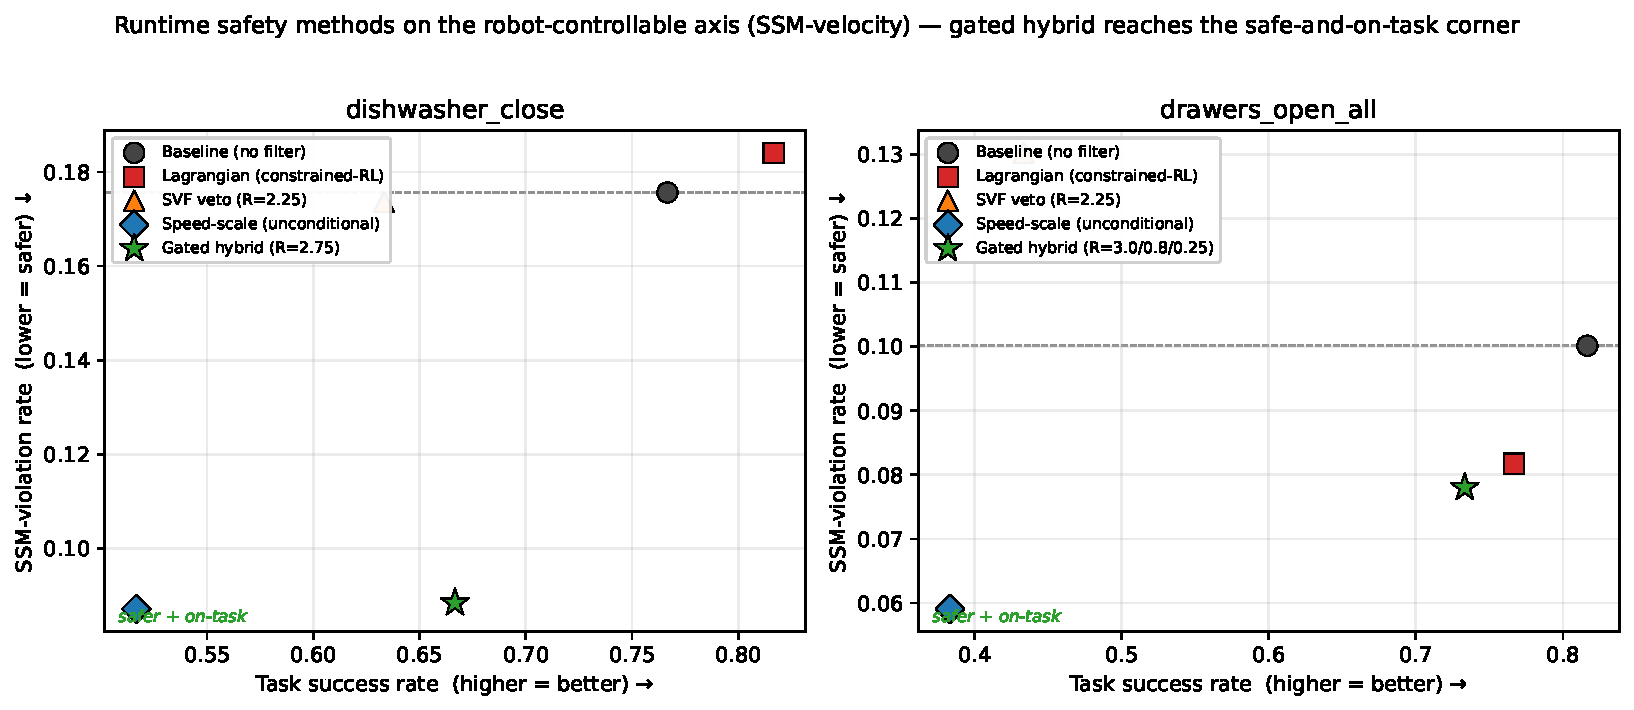
\includegraphics[width=0.75\textwidth]{fig1_method_comparison}
\caption{The intermittent-co-location headline: each method on the
success (x) / \ssm{}-violation (y) plane; the desirable corner is
bottom-right (high success, low violation), and only the
critic-gated filter reaches it on both tasks. Two points need their
context. The \emph{\texttt{drawers\_open\_all} Lagrangian} point sits near the gated
one, but it is a basin-selected checkpoint from seed-unstable,
single-seed training on which no feasible budget exists
(PID-$\lambda$ is inert or task-fatal across the budget sweep);
gating-on-Lagrangian $\approx$ gating-on-baseline (ablation~3,
Section~\ref{sec:results:r2-ablations}) shows it learned no
genuinely proactive avoidance; and it offers no deployable dial,
whereas the gate threshold $R$ traces a tunable frontier
(Figure~\ref{fig:r2-tradeoff}). The \emph{unconditional speed-scale}
points reach the lowest violation rates but at $2.5$--$5\times$ the
gated filter's success cost.}
\label{fig:r2-method-comparison}
\end{figure}

\begin{figure}[htbp]
\centering
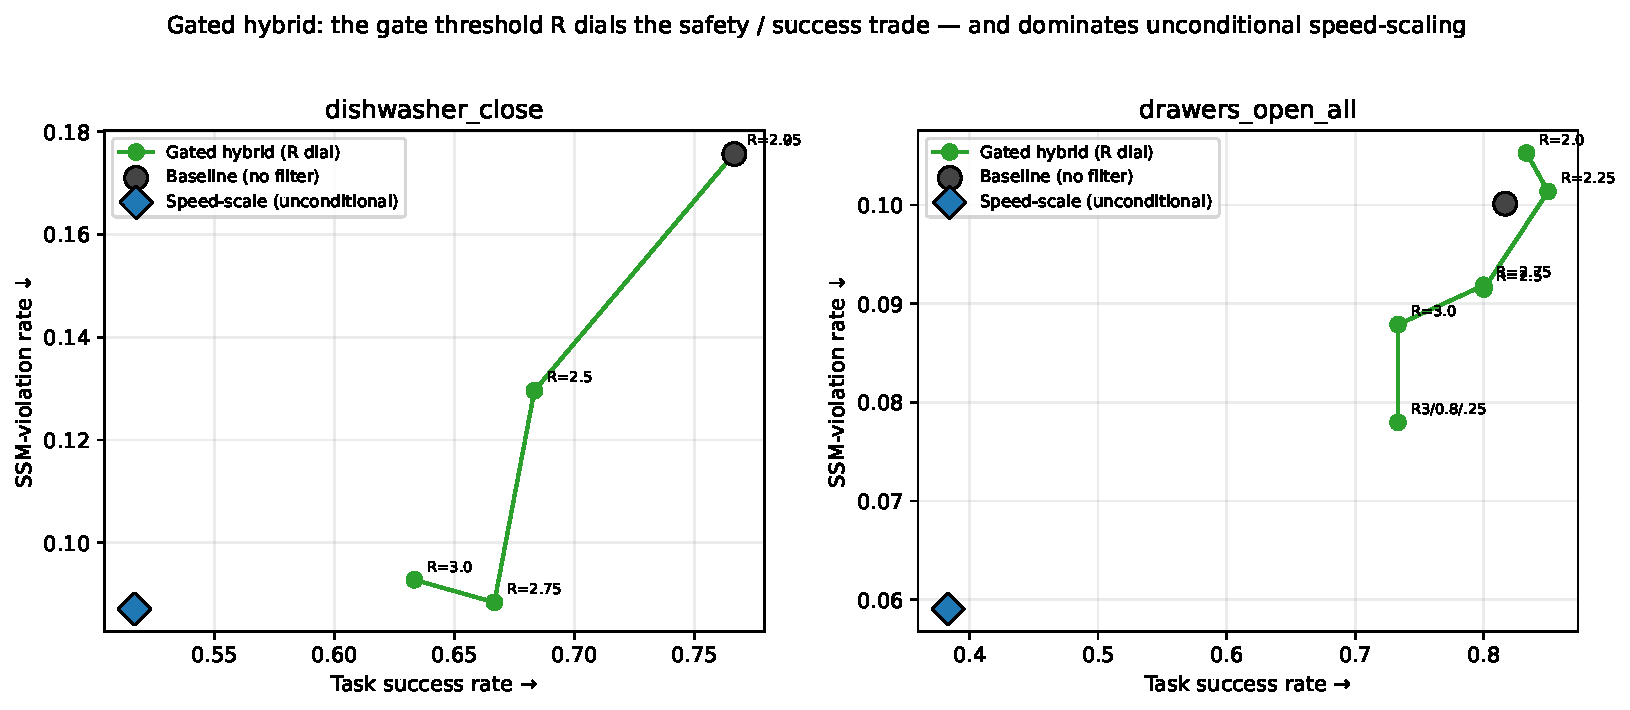
\includegraphics[width=0.7\textwidth]{fig2_tradeoff_curve}
\caption{The gate threshold $R$ is a clean operating-point dial: low
$R$ is selective (near-baseline success, small \ssm{} gain), high $R$
approaches unconditional scaling. The dominance claim is
task-scoped, per the two-axis protocol: on \emph{\texttt{dishwasher\_close}} the gated
frontier matches unconditional scaling's \ssm{}-violation at
strictly higher success; on \emph{\texttt{drawers\_open\_all}} the gated frontier never
reaches unconditional's absolute floor ($0.059$ vs.\ best gated
$0.078$) but pays far less success at every \emph{shared}
\ssm{}-violation level.}
\label{fig:r2-tradeoff}
\end{figure}

The gated result should be read with its scope attached: the gate
recovers throughput \emph{where genuinely-safe windows exist for the
critic to find}. That scope is not a rhetorical hedge; it is the
regime variable, and Section~\ref{sec:results:boundary} measures it
and tests it on a third task.

\subsection{Gate Ablations: Four Refinements Confirm the Recipe}
\label{sec:results:r2-ablations}

Four follow-ups probed whether a better configuration was being
missed; all four converge back on the recommended recipe, and each
yields a portable lesson.

\begin{enumerate}[topsep=2pt,itemsep=2pt]
\item \emph{Pareto surface ($d_{\mathrm{slow}} \times R$,
  \texttt{dishwasher\_close}).} Across $d_{\mathrm{slow}} \in \{0.4, 0.5, 0.6,
  0.8\}$\,m, the gate threshold $R$ is the dominant dial and
  $d_{\mathrm{slow}}$ is secondary ($R = 2.75$ gives $-49$ to
  $-51\,\%$ \ssm{} at $0.63$--$0.67$ success regardless). The
  $R$-sweep \emph{is} the frontier. One interaction matters:
  $R = 3.0$ with $d_{\mathrm{slow}} = 0.4$ re-introduces veto-like
  overshoot (max velocity $6.10$), so $d_{\mathrm{slow}} \geq 0.5$
  is kept, an echo of the veto's coherence break
  (Section~\ref{sec:results:r2-veto}) inside the gated filter
  itself.
\item \emph{Anticipatory critic labels.} Re-labelling the critic at
  looser thresholds ($0.20$ / $0.30$\,m, so it warns earlier) does
  not improve the operating point; the earlier-warning critics slide
  along the same success/safety trade (\texttt{dishwasher\_close} $R = 2.75$:
  $0.63$/$-35\,\%$ and $0.63$/$-44\,\%$ vs.\ the $0.10$\,m critic's
  $0.67$/$-50\,\%$). The most \emph{selective} near-contact label is
  the best gate; anticipation belongs to the policy, not the gate.
\item \emph{Gating on the Lagrangian policy.} Running the gated
  backstop on the best Lagrangian basin checkpoint instead of the
  curriculum baseline is a wash (\texttt{dishwasher\_close} $0.70$/$-36\,\%$ vs.\
  $0.67$/$-50\,\%$; \texttt{drawers\_open\_all} $0.77$/$-25\,\%$ vs.\ $0.80$/$-8\,\%$ at
  matched settings; neither dominates). This is the direct evidence
  that the budget-sweep Lagrangian produced no genuinely
  proactive-avoiding policy on these tasks, and it is what licenses
  the \texttt{drawers\_open\_all} Lagrangian caveat on
  Figure~\ref{fig:r2-method-comparison}.
\item \emph{DAgger-style re-collection on filtered rollouts.}
  Retraining the critic on the \emph{filtered} policy's own rollouts,
  the natural ``fix the distribution shift'' move, is null to
  harmful: the re-collected critic \emph{under}-gates (\texttt{dishwasher\_close}
  $-2\,\%$ \ssm{} vs.\ $-50\,\%$), because the filtered distribution
  already looks safe (the filter slowed the robot during
  collection), so the critic rarely fires. A runtime gate must be
  trained on the \emph{unfiltered} policy's behaviour: it has to
  recognise what the raw policy \emph{would} have done.
\end{enumerate}

\section{The Boundary Condition Across Three Tasks}
\label{sec:results:boundary}

The two preceding sections have opposite headlines. On \texttt{saucepan\_to\_hob}, the
constrained policy is the working mechanism and every runtime filter
pays an unacceptable cost. On \texttt{dishwasher\_close} and \texttt{drawers\_open\_all}, the
critic-gated filter is the working mechanism and constrained RL fails.
This section shows that the two headlines are one finding, and that
the deciding variable is measurable. The closing experiment is the
cross-task gating test (E4.4). It runs the exact intermittent-regime
winner, critic-gated speed-scaling, on \texttt{saucepan\_to\_hob}.
The decision rule was fixed in advance: \emph{the gate counts as
recovering throughput iff some threshold reaches success $\geq 0.60$
and \ssm{}-actual $\leq 0.08$}.

\subsection{The Gate Does Not Recover Throughput on Saucepan}

Table~\ref{tab:e4.4-gated-saucepan} reports the full sweep (the
\texttt{saucepan\_to\_hob} SVF critic, $R \in \{0 \ldots 3.0\}$, plus an on-policy
re-collected critic and the unconditional control; 180 episodes per
row). \textbf{No row passes the pre-registered rule.} As $R$ rises,
the operating point moves monotonically from policy-alone
($0.722$ success, $0.138$ \ssm{}-actual) to the unconditional point
($0.433$, $0.072$); the closest rows are $R = 3.0$ ($0.472$/$0.084$,
below the success floor) and $R = 2.5$ ($0.567$/$0.105$, below both
bars). The gated curve \emph{tracks} the unconditional scaler rather
than dominating it; no high-success, low-violation corner opens.
The decision rule failed on \texttt{saucepan\_to\_hob}, and that outcome was the
\emph{predicted} failure mode under the regime map, not an anomaly to
be explained away.

\begin{table}[htbp]
\centering
\small
\caption{Experiment E4.4. Critic-gated speed-scaling on
\texttt{saucepan\_to\_hob} (180 episodes per row, 3 trained seeds;
\texttt{noisy}). The pre-registered rule, success $\geq 0.60$ \emph{and}
\ssm{}-actual $\leq 0.08$, is met by no row: gating slides from
policy-alone toward the unconditional point without opening a
corner. The on-policy re-collected critic does not help
either; at $R = 2.0$ its \ssm{}-actual ($0.149$) is \emph{worse}
than policy-alone ($0.138$), confirming the limit is task structure,
not critic calibration.}
\label{tab:e4.4-gated-saucepan}
\begin{tabular}{llcccl}
\toprule
Critic / filter & $R$ & Success & Prox.\ viol. & \ssm{}-actual & Reads as \\
\midrule
baseline SVF & 0.0  & 0.722 & 0.271 & 0.138 & policy alone (gate never fires) \\
baseline SVF & 1.5  & 0.717 & 0.299 & 0.127 & gate barely active \\
baseline SVF & 2.0  & 0.706 & 0.295 & 0.125 & \\
baseline SVF & 2.5  & 0.567 & 0.282 & 0.105 & success falling \\
baseline SVF & 2.75 & 0.472 & 0.275 & 0.102 & \\
baseline SVF & 3.0  & 0.472 & 0.283 & 0.084 & approaching unconditional \\
unconditional speed-scaling & --   & 0.433 & 0.276 & 0.072 & gate's $R \to \infty$ limit \\
on-policy SVF & 2.0  & 0.733 & 0.297 & 0.149 & no help \\
on-policy SVF & 2.5  & 0.644 & 0.279 & 0.130 & no help \\
\bottomrule
\end{tabular}
\end{table}

\begin{figure}[htbp]
\centering
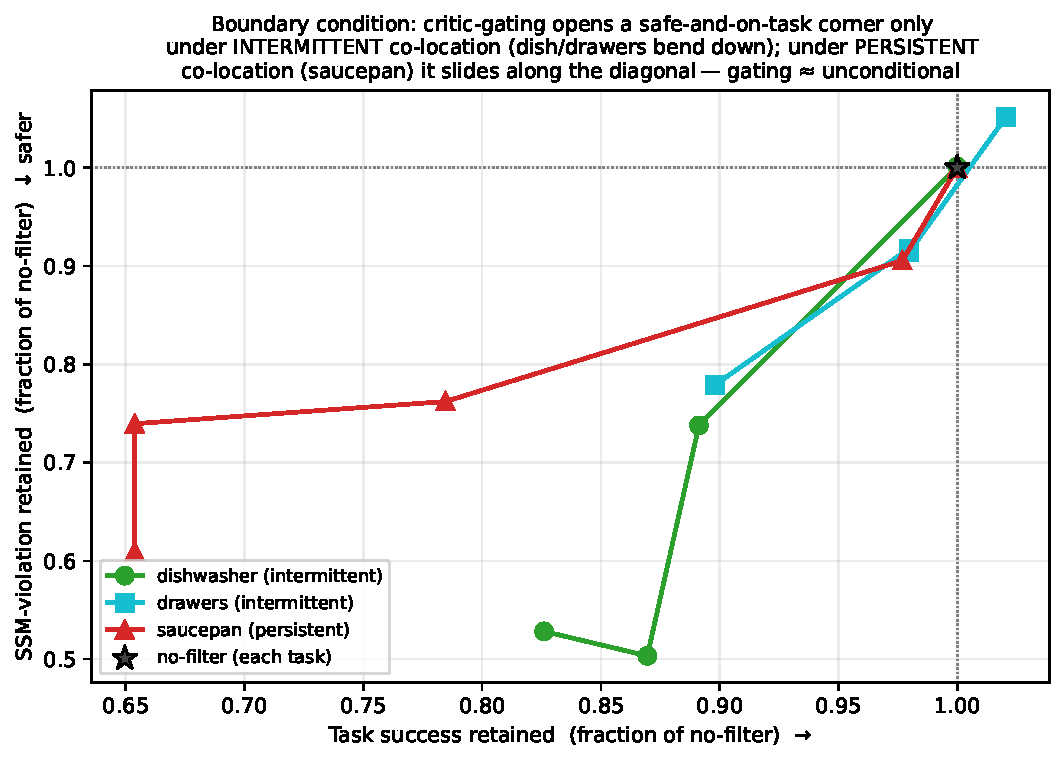
\includegraphics[width=0.72\textwidth]{fig5_cross_task_boundary}
\caption{The boundary condition in one picture: each task's gated
$R$-dial trajectory on the success/\ssm{}-violation plane,
normalised to its own no-filter point. \texttt{dishwasher\_close} and
\texttt{drawers\_open\_all}
\emph{bend down}, \ssm{}-violation falls steeply while success is
retained, because the gate passes the genuinely-safe majority of
steps at full speed. \texttt{saucepan\_to\_hob} \emph{slides along the diagonal}
toward its unconditional endpoint, success and \ssm{}-violation
falling together, because the gate is active on most steps and
gating degenerates to unconditional scaling.}
\label{fig:cross-task-boundary}
\end{figure}

\subsection{The Mechanism, Measured}

The explanation is not asserted from task descriptions. It is measured
from the gate itself (Figure~\ref{fig:gate-activity}). At the matched
threshold $R = 2.75$, the gate is active on $61.5\,\%$
$[57.2, 65.4]$ of steps on \texttt{saucepan\_to\_hob}, versus $26.5\,\%$
$[16.3, 36.7]$ on \texttt{dishwasher\_close} and $19.2\,\%$ $[12.7, 25.3]$ on
\texttt{drawers\_open\_all}; at each task's recommended operating point the contrast is
$51$--$63\,\%$ versus $\approx$27\,\%. On \texttt{saucepan\_to\_hob} the gate fires
\emph{more often} than the unconditional scaler's own proximity
trigger ($44.2\,\%$ of steps within $d_{\mathrm{slow}} = 0.40$\,m):
the critic has no selectivity left to offer, so the ``gated'' filter
is the unconditional filter with extra steps. This is the same
mechanism the persistent-co-location section identified from the
other side, where the
\emph{unconditional} scaler's success floor was traced to a
separation-triggered response that ``fires almost constantly'' under
persistent co-location
(Section~\ref{sec:results:headline-feature-table}). The two arcs of
the two result arcs point to the same boundary condition:

\begin{quote}
\textbf{The boundary condition.} Critic-gated filtering recovers task
throughput when human--robot co-location is intermittent. The gate is
useful because genuinely-safe windows exist and can be passed through
at full speed. Under persistent co-location, those windows disappear.
Every separation-triggered mechanism, gated or not, is active almost
continuously. The remaining lever on the exposure axis is anticipatory
avoidance, which must be trained into the policy.
\end{quote}

\begin{figure}[htbp]
\centering
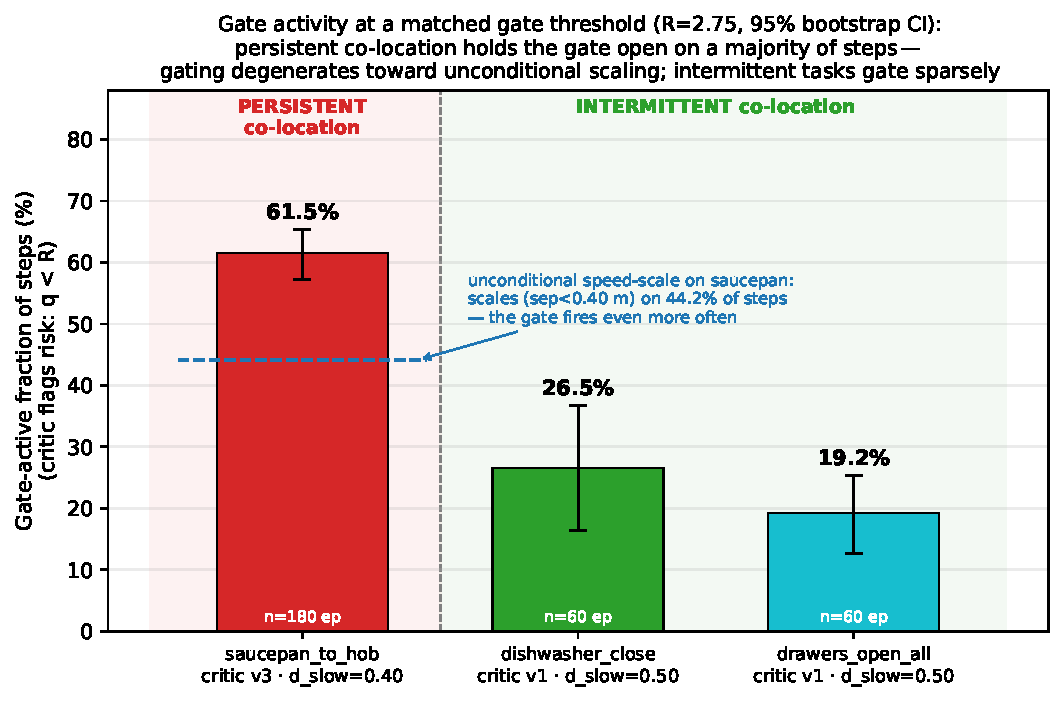
\includegraphics[width=0.58\textwidth]{fig7_gate_activity}
\caption{The regime variable, measured: per-step gate-active
fraction of the critic-gated filter at the matched threshold
$R = 2.75$ (bars; 95\,\% bootstrap CIs; 180/60/60 episodes). The
\texttt{saucepan\_to\_hob} gate fires on $61.5\,\%$ of steps, exceeding even the
unconditional scaler's proximity trigger rate ($44.2\,\%$, dashed),
so gating degenerates to unconditional scaling; on
\texttt{dishwasher\_close}/\texttt{drawers\_open\_all} the gate passes $73$--$81\,\%$ of steps at full
speed, which is exactly the recovered throughput of
Table~\ref{tab:r2-methods}.}
\label{fig:gate-activity}
\end{figure}

\subsection{The Regime Map}

Figure~\ref{fig:regime-map} assembles the full cross-task picture. Two
points matter. First, \textbf{critic-gating does not rescue the
\texttt{saucepan\_to\_hob} composition}. The policy--filter composition's
$0.85 \to 0.44$ success cost (Section~\ref{sec:results:joint-coverage})
stands. An on-policy critic does not change it. E4.4 explains that
ceiling and validates it across tasks, but does not provide a
workaround. Second, the regime map is a deployment rule. Measure or
simulate the co-location pattern first. Then choose the constrained
policy where co-location is persistent, and the critic-gated backstop
where it is intermittent. Do not use a binary veto on a chunked policy.

Table~\ref{tab:recommended-recipes} states the practical recipe implied
by the regime map. A new task should first run a logged or simulated
rollout with the candidate gate and measure the gate-active fraction.
That diagnostic indicates whether the task has enough safe windows for
a runtime gate to preserve throughput.

\begin{table}[htbp]
\centering
\small
\caption{Recommended safety recipe from the regime map. The bands are
empirical ranges from this benchmark, not universal constants.}
\label{tab:recommended-recipes}
\begin{tabular}{lll}
\toprule
Measured gate-active fraction & Regime reading & Recommended mechanism \\
\midrule
$\approx 20$--$30\,\%$ & intermittent co-location & critic-gated speed-scaling \\
$\approx 50$--$65\,\%$ & persistent co-location & train safety into the policy \\
between these bands & uncertain / mixed & sweep both mechanisms and inspect task cost \\
\bottomrule
\end{tabular}
\end{table}

\begin{figure}[htbp]
\centering
\begin{tikzpicture}[
  font=\small,
  regime/.style={draw, rounded corners, align=left, inner sep=7pt,
                 minimum width=0.43\textwidth, text width=0.40\textwidth},
  works/.style={text=green!45!black},
  fails/.style={text=red!60!black},
  lbl/.style={font=\small\bfseries, align=center},
]
\node[regime, fill=blue!4, draw=blue!50] (interm) at (0,0) {%
  \textbf{Intermittent co-location}\\[1pt]
  {\footnotesize \texttt{dishwasher\_close}, \texttt{drawers\_open\_all}}\\[1pt]
  {\footnotesize gate active on $\approx$19--27\,\% of steps}\\[4pt]
  {\footnotesize\textcolor{green!45!black}{\cmark\ critic-gated speed-scaling:
   $-50\,\%$/$-22\,\%$ \ssm{} at $\leq 0.10$ success cost}}\\[2pt]
  {\footnotesize\textcolor{red!60!black}{\xmark\ Lagrangian: no feasible budget
   (inert or task-fatal)}}\\[2pt]
  {\footnotesize\textcolor{red!60!black}{\xmark\ binary veto: chunk-coherence
   break (max vel $2.46 \to 6.03$)}}%
};
\node[regime, fill=orange!6, draw=orange!70!black, right=9mm of interm] (persist) {%
  \textbf{Persistent co-location}\\[1pt]
  {\footnotesize \texttt{saucepan\_to\_hob}}\\[1pt]
  {\footnotesize gate active on $\approx$51--63\,\% of steps}\\[4pt]
  {\footnotesize\textcolor{green!45!black}{\cmark\ constrained policy (fixed
   $\lambda$): $-23\,\%$ prox.-viol.\ at $0.76$ success}}\\[2pt]
  {\footnotesize\textcolor{red!60!black}{\xmark\ reactive proximity filters:
   freeze or flee}}\\[2pt]
  {\footnotesize\textcolor{red!60!black}{\xmark\ critic-gating $\approx$
   unconditional scaling}}\\[2pt]
  {\footnotesize both-axis safety only via composition, at stacked cost
   ($0.85 \to 0.44$)}%
};
% All axis furniture hangs off ONE reference line (the taller box's
% south edge): the boxes have different heights, so anchoring each
% element to its own box slants the arrow and collides the labels.
\coordinate (axL) at (persist.south -| interm.west);
\coordinate (axR) at (persist.south -| persist.east);
\node[font=\scriptsize, anchor=north]
  at ([yshift=-1.5mm]persist.south -| interm.center) {low gate activity};
\node[font=\scriptsize, anchor=north]
  at ([yshift=-1.5mm]persist.south) {high gate activity};
\draw[->, thick, black!60]
  ([yshift=-8.5mm]axL) -- ([yshift=-8.5mm]axR)
  node[midway, below=1mm, font=\footnotesize]
  {co-location persistence (measured: gate-active fraction, Figure~\ref{fig:gate-activity})};
\draw[black!45]
  ([yshift=-17mm]axL) -- ([yshift=-17mm]axR);
\foreach \p/\lab in {0/0\%,0.25/20\%,0.5/40\%,0.75/60\%,1/80\%} {
  \draw[black!45] ($(axL)!\p!(axR)+(0,-17mm)$)
    -- ++(0,-1.2mm)
    node[below,font=\scriptsize] {\lab};
}
\node[lbl, above=3mm of interm.north] {runtime part carries safety};
\node[lbl, above=3mm of persist.north] {policy part carries safety};
\end{tikzpicture}
\caption{The regime map (the thesis in one image). The observable
regime variable, how persistently the coworker is co-located,
measured as the fraction of steps a separation/risk-triggered filter
would be active, determines which part of the Hybrid Safety Critic
carries the safety burden. The boundary was validated by the
pre-registered E4.4 rule, which failed on \texttt{saucepan\_to\_hob} as the
regime map predicted.
Evidence per cell: gated wins
(\S\ref{sec:results:r2-gated}), Lagrangian infeasibility
(\S\ref{sec:results:r2-lagrangian}), veto coherence break
(\S\ref{sec:results:r2-veto}), policy win and composition ceiling
(\S\ref{sec:results:headline-feature-table},
\S\ref{sec:results:joint-coverage}), freeze/flee taxonomy
(\S\ref{sec:results:reactive-taxonomy}), gating $\approx$
unconditional (Table~\ref{tab:e4.4-gated-saucepan}). On the
intermittent tasks the exposure axis itself is left without a
graceful mechanism, bounded by the exogenous floor
(\S\ref{sec:results:r2-lagrangian}).}
\label{fig:regime-map}
\end{figure}

\section{Summary of Results}
\label{sec:results:summary}

\textbf{RQ1, the persistent regime: safety must be trained in.}
Where co-location is persistent, no runtime mechanism reduces
exposure gracefully: vetoes freeze, dodges flee, and every
separation-triggered filter is active on most steps. The
fixed-multiplier constrained policy cuts proximity violations by
$22.8\,\%$ ($0.296 \to 0.228$) at $0.76$ success across three seeds.
The reduction survives noisy, lagged perception and a held-out
coworker distribution ($-31\,\%$ there), while the worst-case
separation tail is exogenous, the coworker's own approach, and is
moved by no mechanism evaluated: proximity \emph{frequency} is
controllable, the single worst approach is not. Both axes at once
are available only by composing policy and graded scaler at a
stacked success cost ($0.85 \to 0.44$), the regime's ceiling.

\textbf{RQ2, the intermittent regime: gate the runtime backstop.}
Where encounters arrive in bursts, constrained RL finds no feasible
budget: the constraint is inert above the natural cost and
task-fatal below it, a binding multiplier makes motion \emph{faster}
(mean velocity $0.44 \to 0.79$\,m/s), and from-scratch WCSAC
corroborates the trainability difficulty externally. A binary veto
breaks chunked-policy coherence (max velocity $2.46 \to 6.03$\,m/s).
The working mechanism is the learned critic gating the graded
speed-scaler: $-50\,\%$ \ssm{}-violation at $-0.10$ success on
\texttt{dishwasher\_close}, $-22\,\%$ at $-0.09$ (or $-10\,\%$ at $-0.02$) on
\texttt{drawers\_open\_all}, with the gate threshold as a deployable dial
(Figure~\ref{fig:r2-reduction-bars}).

\textbf{RQ3, the boundary: co-location persistence decides.} The
gate-active fraction separates the regimes cleanly ($61.5\,\%$ of
steps on \texttt{saucepan\_to\_hob} versus $19$--$27\,\%$ on
\texttt{dishwasher\_close}/\texttt{drawers\_open\_all} at the
matched threshold), it predicts which part carries the safety burden,
and the pre-registered cross-task rule failed where the map
predicts: under persistent co-location, gating degenerates to
unconditional scaling, and constrained-RL feasibility flips across
the same boundary.

\begin{figure}[htbp]
\centering
\begin{tikzpicture}
\begin{axis}[
  ybar,
  width=0.82\textwidth,
  height=0.38\textwidth,
  ymin=0,
  ymax=75,
  ylabel={\ssm{}-actual violation reduction (\%)},
  symbolic x coords={saucepan,dishwasher,drawers},
  xtick=data,
  xticklabels={\texttt{saucepan\_to\_hob},\texttt{dishwasher\_close},\texttt{drawers\_open\_all}},
  x tick label style={rotate=18, anchor=east, font=\footnotesize},
  ymajorgrids=true,
  grid style={black!10},
  nodes near coords,
  nodes near coords style={font=\footnotesize},
  bar width=18pt,
]
\addplot[fill=blue!35, draw=blue!70] coordinates {
  (saucepan,55)
  (dishwasher,50)
  (drawers,22)
};
\end{axis}
\end{tikzpicture}
\caption{Recommended recipe by task, measured on the robot-controllable
\ssm{}-actual axis. \texttt{saucepan\_to\_hob} uses the policy plus
speed-scaling composition ($-55\,\%$ \ssm{}-actual, success
$0.85 \to 0.44$). \texttt{dishwasher\_close} and
\texttt{drawers\_open\_all} use critic-gated speed-scaling
($-50\,\%$ and $-22\,\%$ \ssm{}-actual, success costs $-0.10$ and
$-0.09$ respectively).}
\label{fig:r2-reduction-bars}
\end{figure}
% =============================================================================
% PART V: DISCUSSION, FUTURE WORK, CONCLUSION
% =============================================================================

% =============================================================================
\chapter{Discussion}
\label{ch:disc}
% =============================================================================

\section{What the Answers Mean}
\label{sec:disc:rqs-revisited}

Section~\ref{sec:results:summary} gives the factual answers to the
three research questions. This section adds the interpretation that
does not belong in a results table.

\textbf{On RQ1, the persistent regime.} Two points sit behind the
headline numbers. First, the observation pilot and the perception
sweep together say something sharper than either alone. Adding
human-state observation to an imitation pipeline without a
safety-reward gradient is not a safety mechanism. The channel was
inert or counterproductive under behaviour cloning. Once a constraint
gradient exists, however, the learned avoidance does not depend on
perfect state estimation. It is statistically indistinguishable under
\texttt{oracle} and \texttt{noisy} perception. Imitation methods can
marginalise observations that are uncorrelated with the demonstrated
action. Constrained RL has a use for the channel. Second, the training
lessons travel beyond this benchmark. Fix or schedule the multiplier
when the only feasible budget sits on a feasibility boundary. Select
constrained checkpoints by a safety-aware rule, because peak-success
selection picks \emph{against} the constraint.

\textbf{On RQ2, the intermittent regime.} \emph{Why} the same
constrained method flips from working to inert-or-fatal across
regimes admits a mechanism-level hypothesis, stated as discussion
rather than demonstrated result: persistent co-location makes the
cost signal \emph{dense} (nearly every step carries graded cost, so
the rolling cost moves smoothly and a feasible region exists just
below the inherent cost), while intermittent co-location delivers
cost in sparse bursts, leaving a cliff-shaped budget landscape
(inert on one side, windup on the other) with nothing graded for
the multiplier to push against. Base-task fragility compounds this,
as from-scratch WCSAC corroborates. Both halves are testable, and
the persistence dial (Section~\ref{sec:fw:persistence-dial}) is the
controlled test.

\textbf{On RQ3, the boundary.} The override form decides feasibility.
The gate decides cost. The regime decides whether the gate has
anything to find. The claim is therefore not ``the hybrid dominates''.
It is that each mechanism dominates in its own regime, and that
both-axis safety under persistent co-location has an explicit,
tunable price. No mechanism moves the exogenous tail. Proximity
\emph{frequency} is controllable, but the single closest approach is
not. This is a statement about distance, not necessarily injury risk:
without reliable \pfl{} force measurements, the report cannot say which
exogenous close approaches would exceed contact-force limits. Only a
Power-and-Force-Limiting collision brake (Section~\ref{sec:fw:pfl})
could address that tail. The regime
classification itself rests on three tasks, a limitation examined
below (Section~\ref{sec:disc:regime-threat}).

\section{Threats to Validity}
\label{sec:disc:threats}

This work has well-defined limits. Naming them precisely is part of
the result, because each one bounds where the regime map and the
deployable recipes can be trusted.

\subsection{The \pfl{} Contact-Detection Limitation}
\label{sec:disc:pfl-bug}

\textbf{The \iso{} compliance claim is qualified to ``geometric /
\ssm{}-only.''} The \pfl{} side of the standard requires
biomechanical force monitoring. The project wires the \pfl{} force
limits, cost signal, labeller, and runtime filter end to end. However,
the underlying contact detection mechanism produces
\texttt{data.ncon = 0} for human--robot pairs in MuJoCo despite
geometric overlap. This is a known issue in \bigym{}'s runtime
robot-attachment. Therefore $c^{\pfl}_t \equiv 0$ throughout this
work. Resolving this is the highest-priority infrastructure follow-up
(Section~\ref{sec:fw:pfl}). Without it,
no \pfl{}-side compliance claim in this report is valid. The
contact-force tail metrics originally planned for
Section~\ref{sec:results:tail} are therefore omitted rather than
reported as zero.

This limitation also affects how the exogenous proximity floor should
be read. The floor shows that a robot policy cannot stop a human from
coming close to a stationary robot. It does not prove that every such
close approach is harmful. Some may remain acceptable if contact forces
stay below \pfl{} limits, which this simulator cannot currently
measure.

\subsection{Curriculum Dependence}
\label{sec:disc:curriculum}

The headline results presuppose the three-stage curriculum of
Section~\ref{sec:method:curriculum}. Direct training on the full
\coworker{} disruption collapses to evacuation; every headline
result generalises only to settings where a comparable staged
curriculum is feasible. This is not a fatal limit (curriculum
learning is a standard solution to long-horizon sparse-reward
RL~\cite{narvekar2020curriculum,openai2019solving}), but it
should temper any reading of the architecture as ``trainable from
scratch on arbitrary human-co-located tasks.''

\subsection{Sim-to-Real: Three Orthogonal Gaps}
\label{sec:disc:sim2real}

\textbf{Perception:} the mock-\bodyslampp{} model is calibrated
against published characteristics~\cite{henning2023bodyslampp} but
is not real perception; a rendered-image run feeding a real
estimator is the natural closure
(Section~\ref{sec:fw:realbody}). \textbf{Dynamics:} MuJoCo's H1
differs from the real platform in unmeasured ways. Domain
randomisation~\cite{tobin2017domainrand}
is the standard follow-up and remains the deployed recipe for
real-world humanoid RL~\cite{radosavovic2024humanoid}, and the gap
must be acknowledged before any real-world claim. \textbf{Contact
fidelity:} we found no validation of any rigid-body engine's contact
forces against measured human--robot collision forces.
Simulator validation on real impacts is trajectory-level only and
finds MuJoCo~\cite{todorov2012mujoco} nearly insensitive to its
contact-stiffness parameter~\cite{acosta2022simvalidation}. Industrial
\pfl{} validation relies on physical biofidelic measurement precisely
because simulating constrained contacts is considered
unreliable~\cite{schlotzhauer2022pfl,svarny2020collision}. The
benchmark's contact forces are therefore safety-shaped rather than
safety-validated, even once the \pfl{} detection limitation is
resolved.

\subsection{The Runtime Filter's Role Is Axis- and Regime-Conditional}
\label{sec:disc:filter-role}

The results force a precise statement of what a runtime filter
contributes, narrower than the field's default framing on one side
and broader on the other. \emph{Narrower}: on the proximity
(exposure) axis under persistent co-location, no reactive mechanism
helps gracefully, the fallback sub-study
(Section~\ref{sec:results:filter-pareto}) shows the only
proximity-cutting fallback is a task-abandoning retreat that worsens
the \ssm{}-actual rate, and this freeze-versus-flee limit is one the
runtime-filter literature reaches independently
(Section~\ref{sec:bg:cbf:conservatism}): a worst-case reactive
filter over-restricts to stay safe~\cite{tian2022confidence},
relaxing conservatism is provably benign only for a
least-restrictive filter~\cite{permissivefilter2025}, and trusting a
human-motion model to relax it fails exactly when the human is
unpredictable~\cite{tian2022confidence}, as a co-located coworker
is. The internalisation analysis
(Section~\ref{sec:results:interaction}) adds the composition half: a
learned veto's intervention rate does not fall as the policy learns
to avoid, it rises, because the avoiding policy exits the critic's
calibration distribution. \emph{Broader}: on the velocity axis with
the right override form, the filter is not a backstop but the
\emph{primary} working mechanism wherever co-location is
intermittent, the critic-gated scaler is the best operating point in
the entire evaluation there, and even under persistent co-location
the unconditional scaler is the only route to velocity-axis
compliance, at a price the regime sets. Our contribution is to
establish both halves empirically on a high-DOF manipulator under
\iso{}, and to name the variable that separates them. The reading is
calibrated on the \coworker{} distribution and these base policies; a
distribution with more robot-initiated approaches would shift the
exogenous share and require re-calibrating filter operating points
($R$, $d_{\mathrm{slow}}$) against the deployed policy.

\subsection{Generalisation Scope and the Resolved Cross-Task Transfer}
\label{sec:disc:arch-gen}

The constrained-RL evidence supports the claim that, on the
persistent-co-location task under this backbone, a fixed-$\lambda$
Lagrangian at a feasible budget achieves a reproducible proximity
reduction where both auto-tuned budgets and reactive filters do not
(RQ1). The cost-form ablation bounds the scope: the cost-signal
\emph{form} (continuous vs.\ binary) is not the operative variable,
the budget relative to the task's inherent cost is, so we do not
claim a general ``continuous beats binary'' result. \emph{Cross-task
transfer} of the full \texttt{saucepan\_to\_hob} pipeline (E5.3) resolved
\emph{negative}: on \texttt{dishwasher\_close} and
\texttt{drawers\_open\_all} no budget binds usefully and the best
constrained point is within noise
(Section~\ref{sec:results:r2-lagrangian}). Under the regime map this
negative is informative rather than anomalous, but its converse
limits should be stated equally plainly: ``reproducibly'' in the
persistent-regime headline means across three \texttt{saucepan\_to\_hob} training
seeds, not across
tasks; and whether the fixed-$\lambda$ recipe holds under a
different backbone, a one-shot-intrusion disruption pattern, or a
different embodiment remains untested.

\subsection{External Baseline (WCSAC): Implemented, with Stated Limits}
\label{sec:disc:wcsac-honest}

The WCSAC~\cite{yang2021wcsac} comparison
(Section~\ref{sec:results:wcsac}) is reported with three explicit
limits. (i) \emph{Single seed per cell}: from-scratch SAC is
high-variance, and the anomalous \texttt{dishwasher\_close} $d{=}30$ cell ($0.03$
success at $\lambda = 0$) is best read as that variance, not as a
budget effect; a clean WCSAC trade-off curve needs $\geq 3$ seeds.
(ii) \emph{From-scratch by necessity}: WCSAC is actor-critic and
cannot consume the critic-only warm-start snapshots, so the
comparison conflates ``safe-RL formulation'' with ``demonstration
prior'', which is exactly why it is presented as an external
reference for trainability and not as a like-for-like ablation.
(iii) \emph{Oracle perception at evaluation}, an upper bound with
respect to the noisy condition the project's own methods are
evaluated under. Within those limits the result is robust:
WCSAC's \texttt{dishwasher\_close} success demonstrates the external method is
viable on the easier task, and its uniform \texttt{drawers\_open\_all} failure
corroborates the base-task-fragility reading of the budget-retarget
result (Section~\ref{sec:results:r2-lagrangian}).

\subsection{Evaluation on More Tasks}
\label{sec:disc:regime-threat}

The regime map is supported by three tasks. That is enough to show a
clear pattern, but not enough to claim that the boundary is universal.
More tasks are needed, especially tasks whose co-location pattern lies
between the two regimes studied here.

The main constraint was GPU access. Each additional task requires a
curriculum baseline, safety-filter data, constrained-RL sweeps, runtime
filter sweeps, and snapshot evaluation. The clean follow-up is the
\emph{persistence dial} (Section~\ref{sec:fw:persistence-dial}): hold
one task fixed, change only how long the coworker stays near the robot,
and test whether the recommended mechanism changes with the measured
gate-active fraction.

\subsection{Headline-Architecture Caveat (B-value-mean vs.\ B-CVaR)}
\label{sec:disc:arch-caveat}

The headline architecture is B-value-mean (mean-cost dual-critic).
The standard critique of mean-cost Lagrangian methods is that they
bound only $\mathbb{E}[Z_c]$, not the tail~\cite{yang2021wcsac}. We
report $\cvar_{0.95}$ as a diagnostic and find that the mean-trained
policy's worst-case separation tail is no worse than the baseline's,
but the reason is specific to this setting and does \emph{not} vindicate
mean-cost training in general: the tail here is \emph{exogenous}
(Section~\ref{sec:exogenous}), the human walking into a co-located
robot, so it lies outside what \emph{any} robot-side training
objective, mean or CVaR, can move. A CVaR-trained policy would not
reduce this tail either; the limitation is the reactive control
surface, not the risk measure. On a heavier-tailed cost distribution
whose tail \emph{is} robot-driven (explicit adversarial coworker
behaviours, contact-rich tasks where the robot's own motion creates
the worst case), the mean-trained policy would likely under-perform a
CVaR-trained one, and the future-work direction
(Section~\ref{sec:fw:cvar}) is motivated by that scenario rather than
by this one.

\subsection{Computational Feasibility}
\label{sec:disc:compute}

At 76 DOF, a constraint-projection CBF quadratic program would have to
be constructed and solved over many human-link pairs every control
step, a substantially heavier per-step cost than a single MLP forward
pass and one that additionally requires hand-specified barrier
functions; this project instead uses a learned safety value function
(for the veto) and a closed-form speed-scaling rule as the runtime
filters, both of which are negligible alongside the policy's own
forward pass. The control loop runs at 20\,Hz (a 50\,ms per-step
budget); the policy forward pass, the filter evaluation, and the
fallbacks are simple tensor operations that sit comfortably within
that budget, so no component was separately micro-profiled. The
substantive computational argument is comparative: the learned
filter avoids the per-step QP that a 76-DOF CBF would demand.

\section{Broader Impact}
\label{sec:disc:broader}

\subsection{Responsible Deployment and Misuse Risk}

The strongest practical implication of the regime map is also the main
ethical warning. A runtime safety wrapper can make a learned humanoid
\emph{look} safer without making it certifiably safe. This project
improves measurable \ssm{}-velocity behaviour in simulation. It does
not validate real contact forces, real perception failures, or real
human reactions. A company deploying a humanoid in a home, warehouse,
or care setting could misuse these results by presenting a wrapper as
evidence of ISO compliance. That would be a category error. The
report's claim is narrower: the mechanisms improve specific measured
axes in a simulated co-working benchmark, and the \pfl{} force loop
remains unevaluated.

The regime map adds one concrete pre-deployment check: \emph{measure
the co-location pattern first}. The gate-active fraction of a candidate
filter on logged or simulated traffic is cheap to compute and, on this
evidence, predicts whether critic-gated scaling can recover throughput
or whether persistent co-location will force a heavy safety--throughput
trade. This should be treated as a screening test, not a certificate.
If the pattern is persistent, a deployer should expect either slowed
operation, proactive task replanning, or a redesign of the workspace
rather than a transparent safety layer.

A second lesson, from E4.3, is that validation must be joint. A runtime
filter cannot be assumed to ``hand over'' to a policy trained to be
safe, because the policy may move out of the critic's calibration
distribution. Real-world validation must therefore test the exact
policy--filter composition on the exact deployment distribution, with
the filter re-calibrated whenever the policy, perception stack, task,
or coworker pattern changes.

\subsection{Vulnerable Users and Domestic Environments}

\iso{} targets industrial collaboration, where users are trained,
adult, aware of the robot, and operating under a safety process.
Domestic or care environments violate those assumptions. Children may
approach unpredictably, elderly users or disabled users may have slower
reaction times, and bystanders may not understand the robot's intended
workspace. The exogenous-proximity finding is therefore especially
important: if a vulnerable person walks into a stationary robot, a
robot-side policy cannot remove the exposure, and only a last-resort
\pfl{} brake, physical workspace design, supervision, or external
sensing can reduce the residual risk.

For this reason the report should not be read as a case for deploying
learned humanoid manipulators in unconstrained homes. It is a step
towards evaluating such systems. Extending it to vulnerable-user
deployment would require stricter cost budgets, real BodySLAM++ or
multi-camera perception tests, contact-force validation, emergency-stop
hardware, human-subjects ethics review, and a regulatory answer to
which standard applies outside the industrial-collaboration setting.
The safety--throughput trade should also be disclosed to users: in the
persistent regime, the safer configuration may be substantially slower
or less successful, and hiding that cost would encourage unsafe
expectations about what the robot can do.

\subsection{Reproducibility}

The full reproducibility checklist (Appendix~\ref{app:repro})
documents commit hashes, hyperparameters, dataset versions, and GPU
hours per phase. The codebase is available at
\url{https://github.com/ayushpatel4/safety-bigym-2}. Every numerical
claim in the report is tied to a saved snapshot, benchmark CSV,
aggregation script, or figure-data note.


% =============================================================================
\chapter{Conclusions and Future Work}
\label{ch:conclusion}
% =============================================================================

\noindent
\iso{}-referenced safety for high-DOF humanoid manipulation under
human co-working has not been systematically addressed in the safe-RL
literature. The field has strong ingredients, including constrained RL
and runtime filtering, but it did not have a rule for when each should
be used. This work contributes five linked pieces. First, it gives a
regime map: an empirical rule for matching the safety mechanism to the
human--robot co-location pattern. Second, it gives a two-axis
measurement protocol based on the finding that $\approx$42\,\% of close
proximity is human-driven and outside robot control. Third, it
contributes \sbigym{}, a safety-aware extension of the
\bigym{}~\cite{chernyadev2024bigym} benchmark on which the question can
be asked. Fourth, it re-derives the constrained objective for
critic-only agents in value-based form, with a proved C51 support-bound
condition for dense shaping. Fifth, it gives mechanism-level design
lessons with deployable operating points.

\noindent
Which mechanism helps is governed by the human--robot co-location
regime, not by mechanism sophistication. Under \emph{persistent}
co-location (\texttt{saucepan\_to\_hob}, gate-active
$\approx$62\,\% of steps), only the anticipatory constrained policy
reduces exposure gracefully. A fixed $\lambda = 0.1$ value-based
Lagrangian cuts the proximity-violation rate by $22.8\,\%$
($0.296 \to 0.228$) at $0.76$ success across three seeds. PID
auto-tuning is seed-unstable at the feasibility boundary. Every
reactive filter pays a freeze-or-flee cost on the exposure axis. Both
measured safety axes improve only when the policy is composed with
graded speed-scaling, and that composition has a multiplicative
success cost ($0.85 \to 0.44$). Under \emph{intermittent} co-location
(\texttt{dishwasher\_close}, \texttt{drawers\_open\_all}, gate-active
$19$--$27\,\%$), constrained RL finds no feasible budget. When its
multiplier binds, the robot gets \emph{faster}, not safer. The
from-scratch WCSAC~\cite{yang2021wcsac} reference corroborates the
trainability difficulty. A binary veto breaks chunked-policy coherence
(max velocity $2.46 \to 6.03$\,m/s). The working mechanism is a learned
critic \emph{gating} an \iso{} speed-scaling backstop:
$-50\,\%$ \ssm{}-violation at $-0.10$ success on
\texttt{dishwasher\_close}, and $-22\,\%$ at $-0.09$ on
\texttt{drawers\_open\_all}. The gate threshold is a deployable
dial. The boundary was validated by a pre-registered rule whose failure
case occurred on \texttt{saucepan\_to\_hob}, where gating measurably degenerates to
unconditional scaling. The worst-case separation tail is exogenous and
unmoved by every mechanism. Exposure frequency is controllable. The
single closest approach is not.

\noindent
As humanoid platforms move from research labs into commercial
deployment, principled methods for safety under imperfect perception
and sustained human co-presence are urgently needed. The Unitree G1's
deployment without collaborative-operation
validation~\cite{unitree_g1,hartmann2026iso} is one representative
data point. The most useful output of this work is a decision rule
where the field had only defaults. Runtime filtering is not a universal
safety layer. Constrained RL is not a universal alternative. The
co-location pattern, which is cheap to measure on logged or simulated
traffic, predicts which mechanism is likely to work and what the
safety--throughput trade will cost. The positioning table
(Table~\ref{tab:related-work-comparison}) places the work within the
emerging literature without claiming primacy. The practitioner lessons
are concrete: gate the scaler, do not veto a chunked policy; train the
gate critic on unfiltered rollouts; fix the multiplier when the
feasible budget lies on a boundary; select constrained checkpoints by
a safety-aware rule; and check the support-bounding invariant before
adding dense shaping to a distributional critic.


\section{Future Work}
\label{ch:future}
\label{sec:conclusion:fw}

\subsection{The Persistence Dial: From Regime Map to Causal Test}
\label{sec:fw:persistence-dial}

The single highest-value next experiment, and the named next step of
this project. The regime map currently rests on three tasks in which
co-location persistence co-varies with task identity
(Section~\ref{sec:disc:regime-threat}). The persistence dial removes
the confound: hold the task fixed (\texttt{dishwasher\_close}, the
cheapest), and run the \emph{same} gated $R$-sweep under two
scripted-coworker schedules, the existing intermittent patrol and a
persistent variant in which the coworker's near-zone dwell is
extended to span the episode. The map makes a falsifiable
prediction: the \texttt{dishwasher\_close} bent frontier
(Figure~\ref{fig:cross-task-boundary}) flattens onto the diagonal as
the gate-active fraction rises toward the \texttt{saucepan\_to\_hob} range, with the
transition tracking the measured gate activity rather than any task
property. A confirming result upgrades the boundary condition to a
controlled intervention on the regime variable; a disconfirming one
localises what task identity contributes. The infrastructure exists
(the dwell knobs are \texttt{ParameterSpace} axes,
Table~\ref{tab:coworker-params}); the cost is one gated sweep per
schedule.

\subsection{Closing the Force Loop: Fixing \pfl{}}
\label{sec:fw:pfl}

The highest-priority infrastructure follow-up is to fix \bigym{}'s
runtime robot attachment so that human--robot contacts are exposed via
\texttt{data.ncon}. Until this is done, the project's \iso{}
compliance claim is \ssm{}-only. Once contact detection works, the
existing \sbigym{} infrastructure is ready to use it: the labeller,
cost signal, dataset schema, and runtime filter already read
$c^{\pfl}_t$. This would bring the \pfl{} side of the standard into
scope and make a near-contact collision brake evaluable.

\subsection{Stronger Guarantees: \cvar{} Training and Formal Filters}
\label{sec:fw:cvar}
\label{sec:fw:formal}
\label{sec:fw:fallback}
\label{sec:fw:filter-during-training}

On the training side, the mean-cost headline formulation lifts to an
explicit distributional cost critic
(Section~\ref{sec:method:lagrangian:Bcvar}): a Gaussian
parametrisation (WCSAC-style~\cite{yang2021wcsac}) or quantile head
(QR-DQN-style~\cite{dabney2018qrdqn}). The cost
critic is already C51-shaped, so a parallel head slots in cleanly,
subject to the support invariant of
Proposition~\ref{lem:support-bound} holding for the cost
distribution. The motivating scenario is a cost tail that is
\emph{robot-driven} (contact-rich tasks, adversarial coworkers); on
the current benchmark the tail is exogenous and no risk measure can
move it (Section~\ref{sec:disc:arch-caveat}).

On the runtime side, our filters demonstrate velocity-axis behaviour
empirically but certify nothing. A CBF-QP with a certified barrier
or an HJ-reachability
filter~\cite{bansal2017hamilton,hsu2024safetyfilter} would add
provable separation/velocity guarantees; the concrete obstacles are
a control-affine dynamics model under \emph{exogenous} human motion
and the curse of dimensionality at 76 DOF, and the well-posed target
is the velocity axis, where the filter's role is unambiguous. The
sharpest unmeasured design, surfaced by the literature survey behind
Section~\ref{sec:bg:cbf:conservatism}, combines confidence-aware
fallback~\cite{tian2022confidence} with this report's override
finding: an \emph{anticipatory filter whose conservative fallback is
graded slow-down rather than freeze}, trusting a human-motion model
only under online misspecification monitoring. We found no published
work that measures that combination. Two smaller items complete the
thread: a proportional-damping fallback where a veto is unavoidable,
and the implemented-but-unrun filter-during-training ablation
(Section~\ref{sec:method:lagrangian:filter-train}), expected to
trade fewer catastrophic exploration trajectories for some
robustness cost~\cite{cbfrl2024,shield2025}.

\subsection{Real-Robot Transfer and the Coworker Realism Spectrum}
\label{sec:fw:realbody}
\label{sec:fw:embodiment}

The large-scale extension is a real Unitree~H1, real
\bodyslampp{}~\cite{henning2023bodyslampp} from on-robot RGB + IMU,
and real human collaborators under ethics review with a safety
supervisor in the loop. The open question is whether the regime map
survives deployment. Two nearer-term studies would help first: a
\emph{coworker-aggressiveness spectrum}, sweeping the
\texttt{coworker\_eval} axes continuously, and an
SMPL-H~\cite{romero2017smplh} coworker replication using the
benchmark's body-agnostic selector (Section~\ref{sec:bench:human}).


% =============================================================================
% References
% =============================================================================
\clearpage
\phantomsection
\addcontentsline{toc}{chapter}{Bibliography}
\bibliography{references}

% =============================================================================
% Declarations (departmental requirement; unnumbered; placed after the
% reference list, outside the page-limit window)
% =============================================================================
\clearpage
\chapter*{Declarations}
\addcontentsline{toc}{chapter}{Declarations}

\paragraph{Originality.}
I declare that this report and the work it describes are my own,
carried out under the supervision of Stephen James, and that all
material from other sources, published or unpublished, is
acknowledged and cited in the references.

\paragraph{Use of generative AI.}
Generative AI tools were used as assistive tools for literature search,
code scaffolding, experiment-log summarisation, plotting-script drafts,
\LaTeX{} formatting, and prose drafting/proofreading. They were not
used as an autonomous source of experimental results or as a substitute
for authorial judgement: all citations were checked against primary
sources, all correctness-bearing code was reviewed and tested by the
author, all numerical claims were traced to run logs or CSV artifacts,
and all report prose was edited and endorsed by the author. The full
declaration, including observed failure modes and verification
procedures, is in Appendix~\ref{app:genai}.

\paragraph{Ethics.}
The project involves no human-subjects research and no personal
data; all human-motion data is from the publicly released AMASS
dataset under its research licence. The full ethical considerations,
including the principal risk of over-claiming safety compliance, are
in Appendix~\ref{app:ethics}.

\paragraph{Sustainability.}
Total compute was roughly 450--500~GPU-hours on A100s,
corresponding to approximately 40\,kg~CO\textsubscript{2}e; the
accounting and the practices that bounded it are in
Appendix~\ref{app:sustainability}.

\paragraph{Code and data availability.}
The code is available at
\url{https://github.com/ayushpatel4/safety-bigym-2}; model-weight and
dataset availability are detailed in Appendix~\ref{app:data}.


% =============================================================================
% Appendices (after the reference list and declarations, outside the
% page-limit window).
% =============================================================================
\appendix
% Distinct hyperref anchors for appendix chapters (the chapter counter
% restarts for the main chapters, which would otherwise collide).
\renewcommand*{\theHchapter}{appx.\Alph{chapter}}
% =============================================================================

\chapter{Hyperparameter Tables}
\label{app:hparams}

\section{Phase 2: Offline CQL Safety Critic}
\label{app:hparams:svf}

\begin{table}[htbp]
\centering
\small
\caption{Phase 2 offline CQL safety-value-function hyperparameters.
The dataset is collected under \texttt{noisy} perception because a
runtime filter must learn the conditions it faces at deployment
(Section~\ref{sec:setup:perception-mode}).}
\label{tab:app-hparams-svf}
\resizebox{\textwidth}{!}{%
\begin{tabular}{lll}
\toprule
Hyperparameter & Value & Note \\
\midrule
Architecture & MLP $[256, 256, 256]$ $+$ scaled sigmoid & bounded value head \\
Optimiser & Adam, lr $3\times 10^{-4}$ & \\
CQL regulariser & $\alpha_{\mathrm{CQL}} = 5.0$ & ablated in E2.1 \\
Target violation rate & $0.30$ & matches $\tau_{\mathrm{prox}}$ calibration \\
Discount & $\gamma = 0.99$ & \\
Target-net Polyak & $\tau = 0.005$ & \\
Dataset & \cqnas{} rollouts, \texttt{coworker\_train}, \texttt{noisy} & labelled at $\tau_{\mathrm{prox}}{=}0.3$\,m ($\sim$16.8\,\% unsafe) \\
Sampler & violation-balanced, target $1{:}1$ & \\
Training / batch & 200{,}000 steps / 512 & \\
\bottomrule
\end{tabular}%
}
\end{table}

The four collection-versus-deployment faithfulness fixes that make
this critic's deployment decisions valid (action de-normalisation,
execution-mode matching, the $500 \rightarrow 20$\,Hz control-frequency
root cause, and coworker-scenario alignment) are described in
Section~\ref{sec:impl:svf-faithful}; the $R = 0$ sweep agreement
($0.286 \approx 0.296$) is the validation that the fixes succeeded.

\section{Phase 3: Constrained Lagrangian Agent (Headline: Fixed $\lambda$)}
\label{app:hparams:lagrangian}

Table~\ref{tab:app-hparams-lagrangian} gives the headline
configuration. The headline multiplier is \emph{fixed} at
$\lambda = 0.1$; the PID gains below are used \emph{only} for the
E3.2 auto-tuning runs that establish the seed-instability finding
(Section~\ref{sec:results:budget}), and are set to zero for the
headline. There is no active cost budget $d$ in the headline, because
pinning $\lambda$ removes the dual-update loop entirely; $d = 0.3$ is
the budget used in the PID-ablation runs.

\begin{table}[htbp]
\centering
\small
\caption{Phase 3 headline hyperparameters (fixed-$\lambda$
constrained \cqnas{}). The cost critic is fully decoupled (its own
optimiser and its own features, the RoboBase shared-encoder
constraint) and cold-started.}
\label{tab:app-hparams-lagrangian}
\resizebox{\textwidth}{!}{%
\begin{tabular}{lll}
\toprule
Group & Value & Note \\
\midrule
\cqnas{} backbone & C51, 101 atoms, $\gamma = 0.99$ & \cite{seo2024cqnas} \\
Value support & $v_{\min} = -6$, $v_{\max} = +2$ & satisfies Prop.~\ref{lem:support-bound} \\
Cost critic & mirrored C51, same support & decoupled optimiser \& features; cold-started \\
Replay / batch / stack & 1M / 256 / 4 & \\
Demonstrations & $\text{num\_demos} = 36$ & \\
\textbf{Multiplier (headline)} & \textbf{fixed $\lambda = 0.1$} & dual loop removed \\
PID gains (E3.2 ablation only) & $K_I{=}10^{-3}, K_P{=}10^{-2}, K_D{=}0$ & $\lambda_{\max}{=}100$; zero in headline \\
Cost budget (E3.2 ablation only) & $d = 0.3$ & not active in headline \\
Workspace shaping & $\beta{=}0.05, r_{\mathrm{ws}}{=}0.4$\,m, $c_{\mathrm{ws}}{=}1.0$\,m & confound-controlled (E4.1) \\
Lagrangian fine-tune & up to 40{,}000 frames & on the stage-2 base \\
Checkpoint selection & \textbf{safety-aware} & lowest deploy proximity at success floor $0.75$ \\
Eval interval & 2{,}000 frames, 20 eval ep & basin at $\sim$20k--35k frames \\
\bottomrule
\end{tabular}%
}
\end{table}

\section{Phase 4: Per-Regime Deployment Configurations}
\label{app:hparams:hybrid}

The deployed runtime configuration is regime-dependent
(Section~\ref{sec:results:boundary}). On the persistent-co-location
task, the both-axis configuration is the fixed-$\lambda$ policy
composed with \emph{unconditional} graded speed-scaling
($d_{\mathrm{slow}} = 0.40$\,m); gating does not help there. On the
intermittent-co-location tasks the deployment filter is
\emph{critic-gated} speed-scaling at the recommended per-task
operating points. The learned SVF \emph{veto} ($R = 2.25$,
$\alpha_{\mathrm{CQL}} = 5.0$) is a negative result everywhere
(velocity backstop at best, OOD on the avoiding policy, coherence
break on chunked policies) and is never the deployment filter;
Table~\ref{tab:app-hparams-hybrid} lists the configurations.

\begin{table}[htbp]
\centering
\small
\caption{Recommended runtime deployment configuration per
co-location regime, as established by the results chapter: the
constrained policy carries safety under persistent co-location, the
critic-gated speed-scaler under intermittent co-location. The veto
and the model-based dodges are taxonomy points, not deployment
configurations.}
\label{tab:app-hparams-hybrid}
\resizebox{\textwidth}{!}{%
\begin{tabular}{llll}
\toprule
Task (regime) & Filter & Operating point & Critic \\
\midrule
\texttt{saucepan\_to\_hob} (persistent) & uncond.\ speed-scaling on fixed-$\lambda$ policy & $d_{\mathrm{slow}}{=}0.40$, $d_{\mathrm{stop}}{=}0.15$\,m & none (ungated) \\
\texttt{dishwasher\_close} (intermittent) & \textbf{critic-gated speed-scaling} & $R{=}2.75$, $d_{\mathrm{slow}}{=}0.50$, $d_{\mathrm{stop}}{=}0.15$\,m & shared intermittent SVF \\
\texttt{drawers\_open\_all} (intermittent) & \textbf{critic-gated speed-scaling} & $R{=}3.0$, $d_{\mathrm{slow}}{=}0.80$, $d_{\mathrm{stop}}{=}0.25$\,m & shared intermittent SVF \\
\texttt{drawers\_open\_all} (near-free option) & critic-gated speed-scaling & $R{=}2.75$, $d_{\mathrm{slow}}{=}0.80$\,m & shared intermittent SVF \\
(all tasks) SVF veto & negative result; not deployed & $R{=}2.25$ & per-task SVF \\
(\texttt{saucepan\_to\_hob}) model-based dodge & taxonomy point (flee); not deployed & $d_{\mathrm{target}}{=}0.35$\,m & none \\
\bottomrule
\end{tabular}%
}
\end{table}

\paragraph{Shared \texttt{dishwasher\_close}/\texttt{drawers\_open\_all} SVF critic.}
Same architecture and CQL recipe as Table~\ref{tab:app-hparams-svf},
trained once for both tasks: 52{,}794 transitions
(random $+$ on-policy curriculum rollouts under \coworker{}),
near-contact label at $\min$-separation $< 0.10$\,m, 200k training
steps. Anticipatory-label variants (0.20/0.30\,m) and a
DAgger-style re-collection on filtered rollouts were trained and
rejected by the ablations of
Section~\ref{sec:results:r2-ablations}.

\paragraph{WCSAC external baseline.}
Faithful reimplementation of~\cite{yang2021wcsac}: Gaussian
distributional cost critic, $\cvar{}_{\alpha}$ constraint with
$\alpha = 0.9$, budgets $d \in \{5, 15, 30\}$ on the discounted cost
return, adaptive multiplier ($\lambda_{\max} = 100$); trained from
scratch ($\text{num\_demos} = 0$), 150k frames, single seed per
cell; evaluated with identity action-normalisation statistics
(Section~\ref{sec:method:wcsac}) over 30 episodes per cell under
\texttt{oracle} perception.

\chapter{Reproducibility Checklist}
\label{app:repro}

\begin{description}[leftmargin=2em,style=nextline]
\item[Code] \url{https://github.com/ayushpatel4/safety-bigym-2}.
  Headline experiments were run from the \texttt{phase3}
  branch at commit \texttt{b3b2ce5}; in addition, the
  snapshot-evaluation harness stamps the exact git SHA into every
  benchmark CSV row, so each reported cell is traceable to the code
  that produced it.
\item[Upstream assets] \bigym{}~\cite{chernyadev2024bigym} provides
  the base simulator, task suite, and demonstrations. AMASS~\cite{mahmood2019amass}
  (CMU subset, downloaded 18 February 2026) drives the
  demonstration-replay human-state channel. \cqnas{}~\cite{seo2024cqnas}
  is vendored at upstream commit \texttt{8cf806e}
  (Section~\ref{sec:impl:integration}).
\item[Hardware and software] A single NVIDIA A100 (40\,GB), CUDA 12.8,
  PyTorch 2.10.0; MuJoCo via \bigym{}. Every script has a CPU-only
  smoke gate (Section~\ref{sec:setup:smoke}).
\item[Seeds] Trained seeds $\{0, 1, 2\}$ for all three-seed cells;
  evaluation uses seeds $\{0, 1, 2\}$ with 20 episodes each
  (Section~\ref{sec:setup:stats}).
\item[Headline recipe (R1)] (i) Train the three-stage curriculum
  (Table~\ref{tab:curriculum-stages}; $\approx$19\,h). (ii) Fine-tune
  with fixed $\lambda = 0.1$ for up to 40k frames per seed
  ($\approx$9\,h each; Table~\ref{tab:app-hparams-lagrangian}).
  (iii) Benchmark every saved checkpoint and select per seed by the
  safety-aware rule (lowest deployment proximity-violation rate at success
  $\ge 0.75$), which yields the headline checkpoints
  \texttt{lam0p1\_seed\{0,1,2\}} at steps 30{,}546 / 8{,}225 /
  32{,}696. (iv) Reproduce
  Table~\ref{tab:e4.1-feature-incremental} by running
  \texttt{scripts/benchmark\_policy.py} on those checkpoints
  (minutes per cell; no retraining).
\item[Headline recipe (R2/R3)] All intermittent-co-location and
  boundary numbers are snapshot evaluations through the same
  harness: the budget sweep via
  \texttt{scripts/dispatch\_budget\_sweep.py} (artifacts under
  \texttt{results/budget\_sweep\_eval/}); the veto, unconditional,
  gated, and ablation sweeps under \texttt{results/\{svf\_sweep,
  speedscale, gated\_sweep, improve, anticipatory\_sweep,
  dagger\_sweep\}/}; the boundary sweep via
  \texttt{scripts/dispatch\_gated\_saucepan.py} (under
  \texttt{results/e4\_1/gated\_saucepan/}); WCSAC via
  \texttt{scripts/dispatch\_wcsac.py} and
  \texttt{scripts/eval\_wcsac.sh} (under
  \texttt{results/wcsac\_eval/}). Figures regenerate via
  \texttt{scripts/make\_report\_figures.py} and
  \texttt{scripts/make\_f7\_gate\_activity.py}.
\item[Hyperparameters] Appendix~\ref{app:hparams}; the Hydra configs
  in the repository pin every value not listed there.
\end{description}

\chapter{Experiment Code Index}
\label{app:exp-index}
\label{sec:setup:exp-index}

Experiments are referred to in the body of the report by what they
show; the repository, run logs, and figure-data notes identify them
by phase-prefixed codes (E$n.m$), stated once in parentheses where
each experiment is reported. Table~\ref{tab:experiment-index} maps
the codes to the report sections carrying their evidence.

\begin{table}[htbp]
\centering
\caption{Experiment index. Each is identified by a phase-prefixed
code (E$n.m$) and reported in Chapter~\ref{ch:eval}; R1 = persistent
co-location (\texttt{saucepan\_to\_hob}), R2 = intermittent
co-location (\texttt{dishwasher\_close}, \texttt{drawers\_open\_all}),
R3 = the cross-task boundary condition.}
\label{tab:experiment-index}
\small
\begin{tabular}{lll}
\toprule
ID & Description & Reported in \\
\midrule
E1.1   & BC observation ablation (off / oracle / noisy), no penalty
       & \S\ref{sec:results:obs-bc} \\
E2.1--E2.3 & SVF CQL-$\alpha$ / filter-on-baseline / threshold-$R$ Pareto (R1)
       & \S\ref{sec:results:filter-pareto} \\
E2.4   & SVF binary veto on the chunked policy (R2)
       & \S\ref{sec:results:r2-veto} \\
E2.5   & Unconditional speed-scaling (R2)
       & \S\ref{sec:results:r2-uncond} \\
E2.6   & Critic-gated speed-scaling, $R$-dial sweep $+$ ablations (R2)
       & \S\ref{sec:results:r2-gated}, \S\ref{sec:results:r2-ablations} \\
E3.1   & Cost-signal form vs.\ budget feasibility (R1)
       & \S\ref{sec:results:cost-signal} \\
E3.2   & Cost budget sweep and feasibility boundary (R1)
       & \S\ref{sec:results:budget} \\
E3.3   & Cost-budget retarget sweep, $d \in \{0.16, 0.19, 0.22\}$ (R2)
       & \S\ref{sec:results:r2-lagrangian} \\
E3.6   & Perception robustness (oracle vs.\ noisy) of the constrained policy
       & \S\ref{sec:results:obs-rl} \\
E3.7   & External baseline: WCSAC, from scratch, 2 tasks $\times$ 3 budgets
       & \S\ref{sec:results:wcsac} \\
E4.1   & \textbf{R1 headline: proactive / reactive / composed comparison}
       & \S\ref{sec:results:headline-feature-table} \\
E4.3   & Filter intervention rate during Lagrangian training (R1)
       & \S\ref{sec:results:interaction} \\
E4.4   & \textbf{R3: critic-gated scaling on \texttt{saucepan\_to\_hob} (pre-registered rule)}
       & \S\ref{sec:results:boundary} \\
E5.1   & Tail-risk metrics across the headline configurations (R1)
       & \S\ref{sec:results:tail} \\
E5.2   & OOD generalisation on the wider \texttt{coworker\_eval} band (R1)
       & \S\ref{sec:results:ood} \\
E5.3   & Cross-task transfer of the \texttt{saucepan\_to\_hob} pipeline (resolved negative)
       & \S\ref{sec:results:r2-lagrangian} \\
\bottomrule
\end{tabular}
\end{table}

\chapter{Benchmark Usage Example}
\label{app:benchmark-usage}

The benchmark is intended to be used from saved policy snapshots. A
typical evaluation command specifies the task, coworker distribution,
observation mode, and policy checkpoint, then writes one CSV row per
evaluation cell:

\begin{verbatim}
python scripts/benchmark_policy.py \
  --task saucepan_to_hob \
  --disruption coworker_train \
  --obs-mode noisy \
  --snapshot results/policies/lam0p1_seed0.pt \
  --episodes 20 \
  --seeds 0 1 2 \
  --out results/benchmark/saucepan_lam0p1.csv
\end{verbatim}

A user-supplied method only has to implement the policy interface that
returns an action for each observation. The harness provides the same
environment, coworker sampler, perception wrapper, and safety metrics
used in this report. A representative output row contains:

\begin{verbatim}
task,disruption,obs_mode,policy,success_rate,episode_reward,
ep_proximity_violation_rate,ep_ssm_violation_actual_rate,
ep_min_separation,ep_mean_separation,intervention_rate
\end{verbatim}

This output is enough to reproduce the report's core comparisons:
task success, exposure to close human--robot proximity, robot
velocity-safety near the human, and the cost of any runtime filter.

\chapter{Frame-by-Frame Walkthroughs}
\label{app:walkthroughs}

This appendix illustrates, frame by frame, the coworker behaviour the
benchmark generates and how the report's main safety mechanisms act on
it, for readers who want to \emph{see} the dynamics behind the result
tables. All four figures share the same episode scenario (seed, coworker
parameters, camera) and the same HUD convention: each panel shows
episode time, the closest-pair separation, and its status against
$\tau_{\mathrm{prox}} = 0.3$\,m; red borders mark steps in proximity
violation. The one deliberate exception is the speed-scaling
walkthrough (Figure~\ref{fig:speedscale-mechanism}), whose borders and
status chips are keyed to the \ssm{}-actual \emph{velocity} violation,
the axis that filter targets, because its geometric proximity is
unchanged by design.

\section{The \coworker{} Patrol Episode}
\label{app:patrol-episode}

Section~\ref{sec:bench:coworker:traj} describes the three \coworker{}
trajectory modes in the abstract. This section shows what the dominant
mode, \textsc{coworker-patrol}, looks like over a single episode.
Figure~\ref{fig:coworker-patrol} composes eight rendered frames over
the episode's separation trace: the walk-in, the reach cycles at
\textsc{near} that cause proximity violations, the depart to
\textsc{away} that opens a safe working window, and the return that
closes it again. This is the rhythm of interruption and opportunity
that the benchmark's training and evaluation distributions are built
around (Section~\ref{sec:bench:coworker}).

\begin{figure}[htbp]
\centering
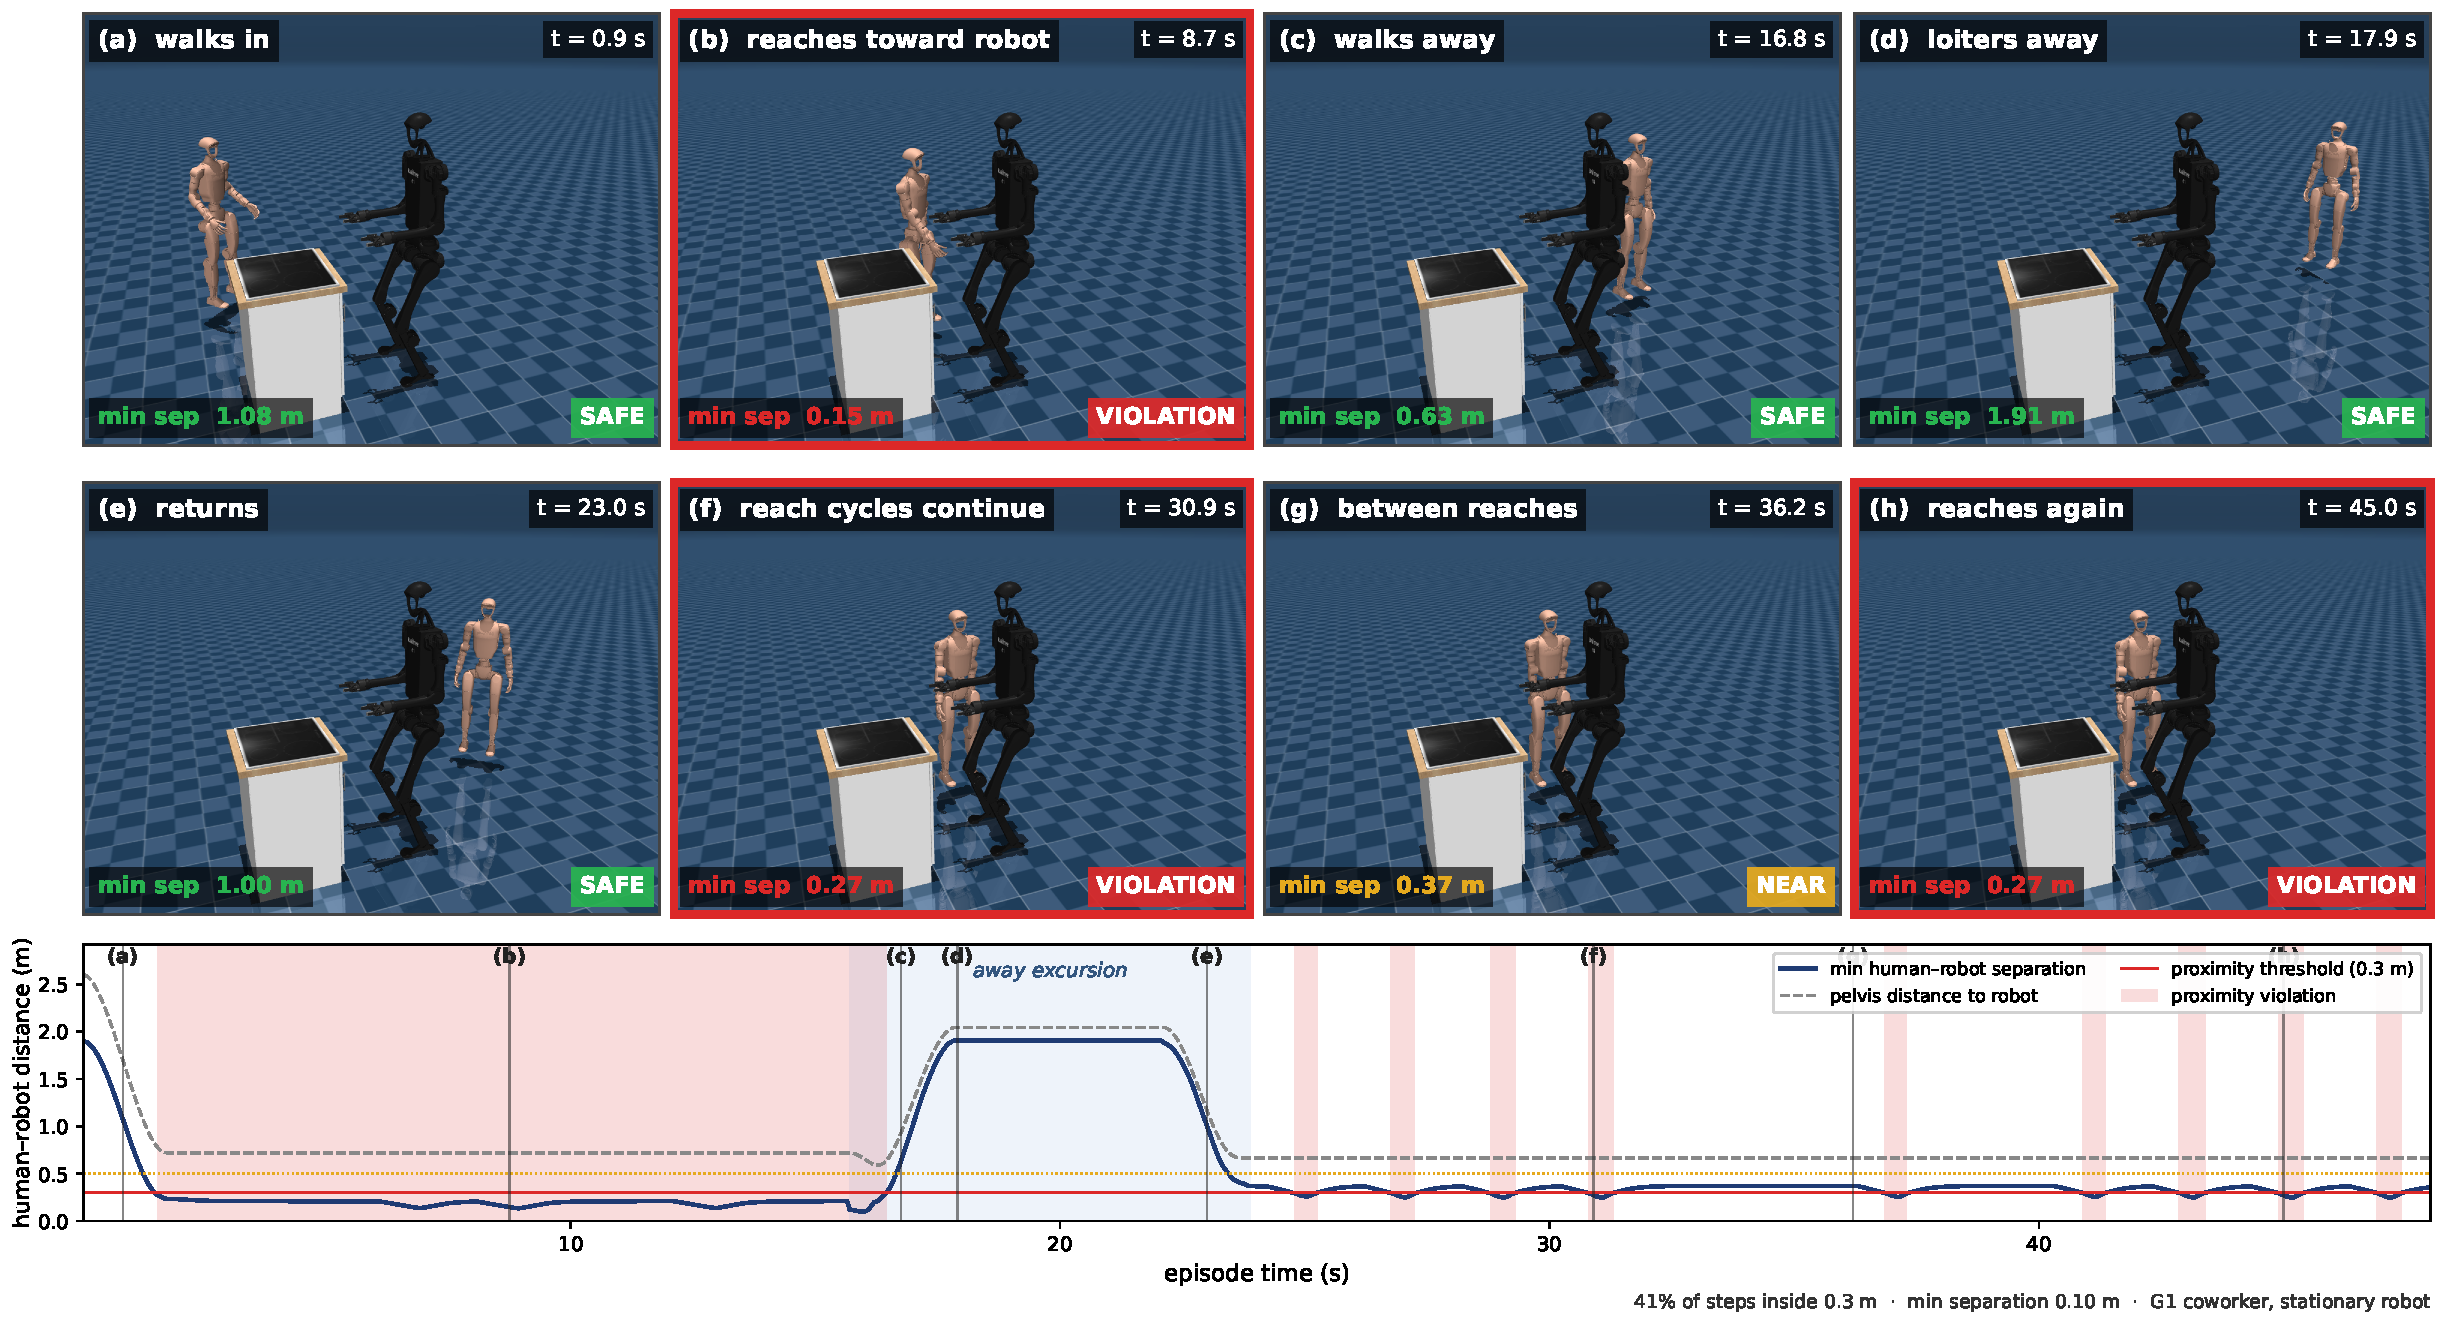
\includegraphics[width=\textwidth]{fig_coworker_patrol_disruption}
\caption{One complete \coworker{} patrol episode, frame by frame
(\texttt{saucepan\_to\_hob}, G1 coworker, stationary robot;
training-band parameters with closest approach $0.72$\,m, reach-target
mix $p_{\mathrm{EE}} = 0.7$, reach period $2.0$\,s). Panels: the
coworker walks in (a) and holds reaches toward the robot's arm and the
task object, driving the closest-pair separation to $0.15$\,m, well
inside $\tau_{\mathrm{prox}} = 0.3$\,m (b); departs (c) to the
\textsc{away} position (d), giving the robot a safe window; returns (e)
to a new \textsc{near} pose and resumes reach cycles (f, h), with
separation recovering above the threshold between reaches (g). Each
panel's HUD shows episode time, closest-pair separation, and status
against $\tau_{\mathrm{prox}}$; red borders mark proximity violations.
Bottom: closest-pair separation (solid) and pelvis distance (dashed)
over the episode; red bands mark proximity violations and the blue band
the \textsc{away} excursion. Over this episode $41\,\%$ of steps fall
inside $0.3$\,m, with minimum separation $0.10$\,m. The robot holds its
home pose (zero-action policy) so every violation is attributable to
the coworker's behaviour; the scenario parameters sit inside the
\coworker{} train band and the episode seed was selected to show a
complete depart--return cycle
(\texttt{scripts/render\_disruption\_figure.py}).}
\label{fig:coworker-patrol}
\end{figure}

\section{Proactive Avoidance: Lagrangian versus Baseline}
\label{app:walk-lagrangian}

Figure~\ref{fig:lagrangian-vs-baseline} contrasts the two behaviours
behind the headline persistent-regime result
(Section~\ref{sec:results:filter-pareto}): the unconstrained baseline
holds its task posture straight through the coworker's reach windows,
while the fixed-$\lambda = 0.1$ Lagrangian yields the base away as the
coworker closes in and returns to the task once they depart, showcasing graceful
avoidance rather than freezing or fleeing.

\begin{figure}[htbp]
\centering
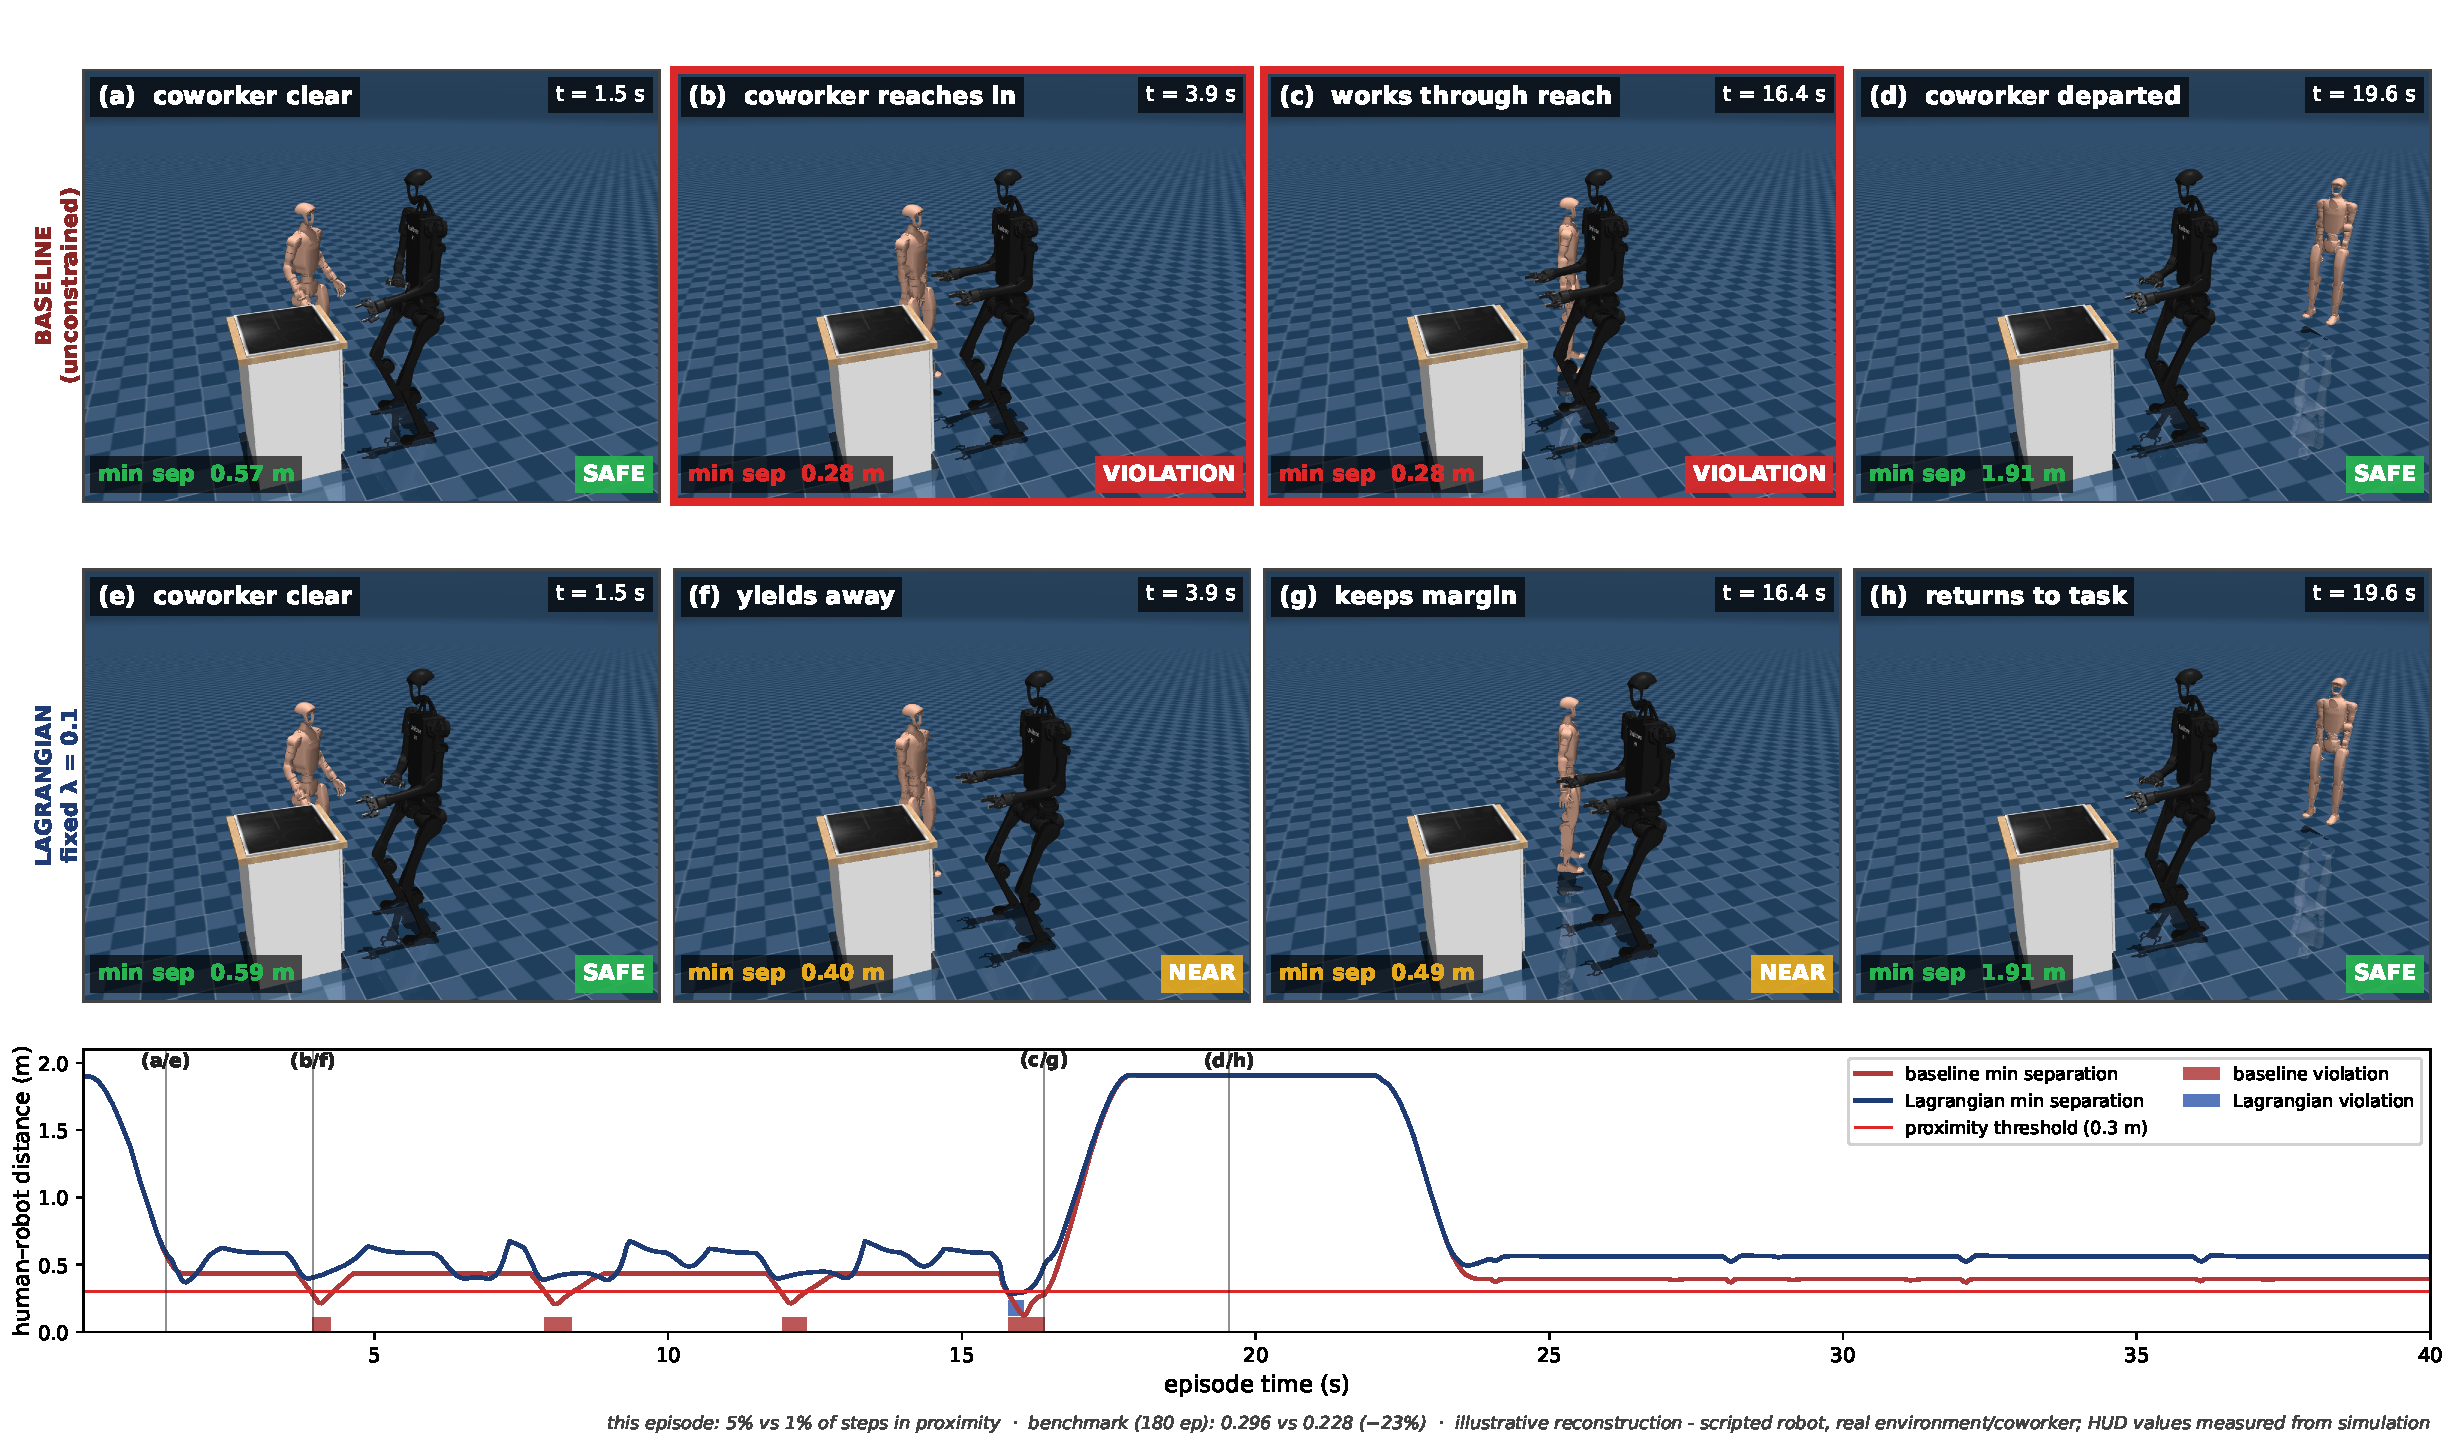
\includegraphics[width=\textwidth]{fig_lagrangian_vs_baseline}
\caption{Proactive avoidance, frame by frame (illustrative
reconstruction; same episode scenario as
Figure~\ref{fig:coworker-patrol}). Top row: the unconstrained baseline
keeps working at the counter through the coworker's reaches — the
closest-pair separation falls to $0.18$\,m and repeated proximity
violations accumulate (red borders, red bands in the timeline). Bottom
row: from the same scenario, the constrained policy's signature
behaviour. It yields the base away when the coworker closes in
(f--g), holds an amber-margin distance instead of a red violation, and
returns to the task when the coworker departs (h). Timeline: both
separation traces with per-policy violation ribbons. In the benchmark
this graceful avoidance gives proximity-violation rate $0.228$ vs
$0.296$ ($-23\,\%$) at success $0.76$ over $180$ episodes
(Section~\ref{sec:results:headline-feature-table},
Figure~\ref{fig:fixlam}).}
\label{fig:lagrangian-vs-baseline}
\end{figure}

\section{The Reactive SVF Veto: Classification and Fallbacks}
\label{app:walk-veto}

Figure~\ref{fig:svf-veto-anatomy} walks through one veto event of the
learned safety-value-function filter
(Section~\ref{sec:results:reactive-taxonomy}). The filter scores every
proposed action, $\hat{Q}(s,a)$ against the threshold $R = 2.25$:
clear-coworker actions PASS unchanged, while a reach-window action is
vetoed and replaced by the fallback. Branching the \emph{same} veto
state three ways exposes the freeze-versus-flee dilemma: executing the
original action walks into proximity. The zero-velocity fallback stops
the robot, which then \emph{dwells} in the danger zone the coworker
creates. The retreat fallback buys separation only by abandoning the
task at high velocity.

\begin{figure}[htbp]
\centering
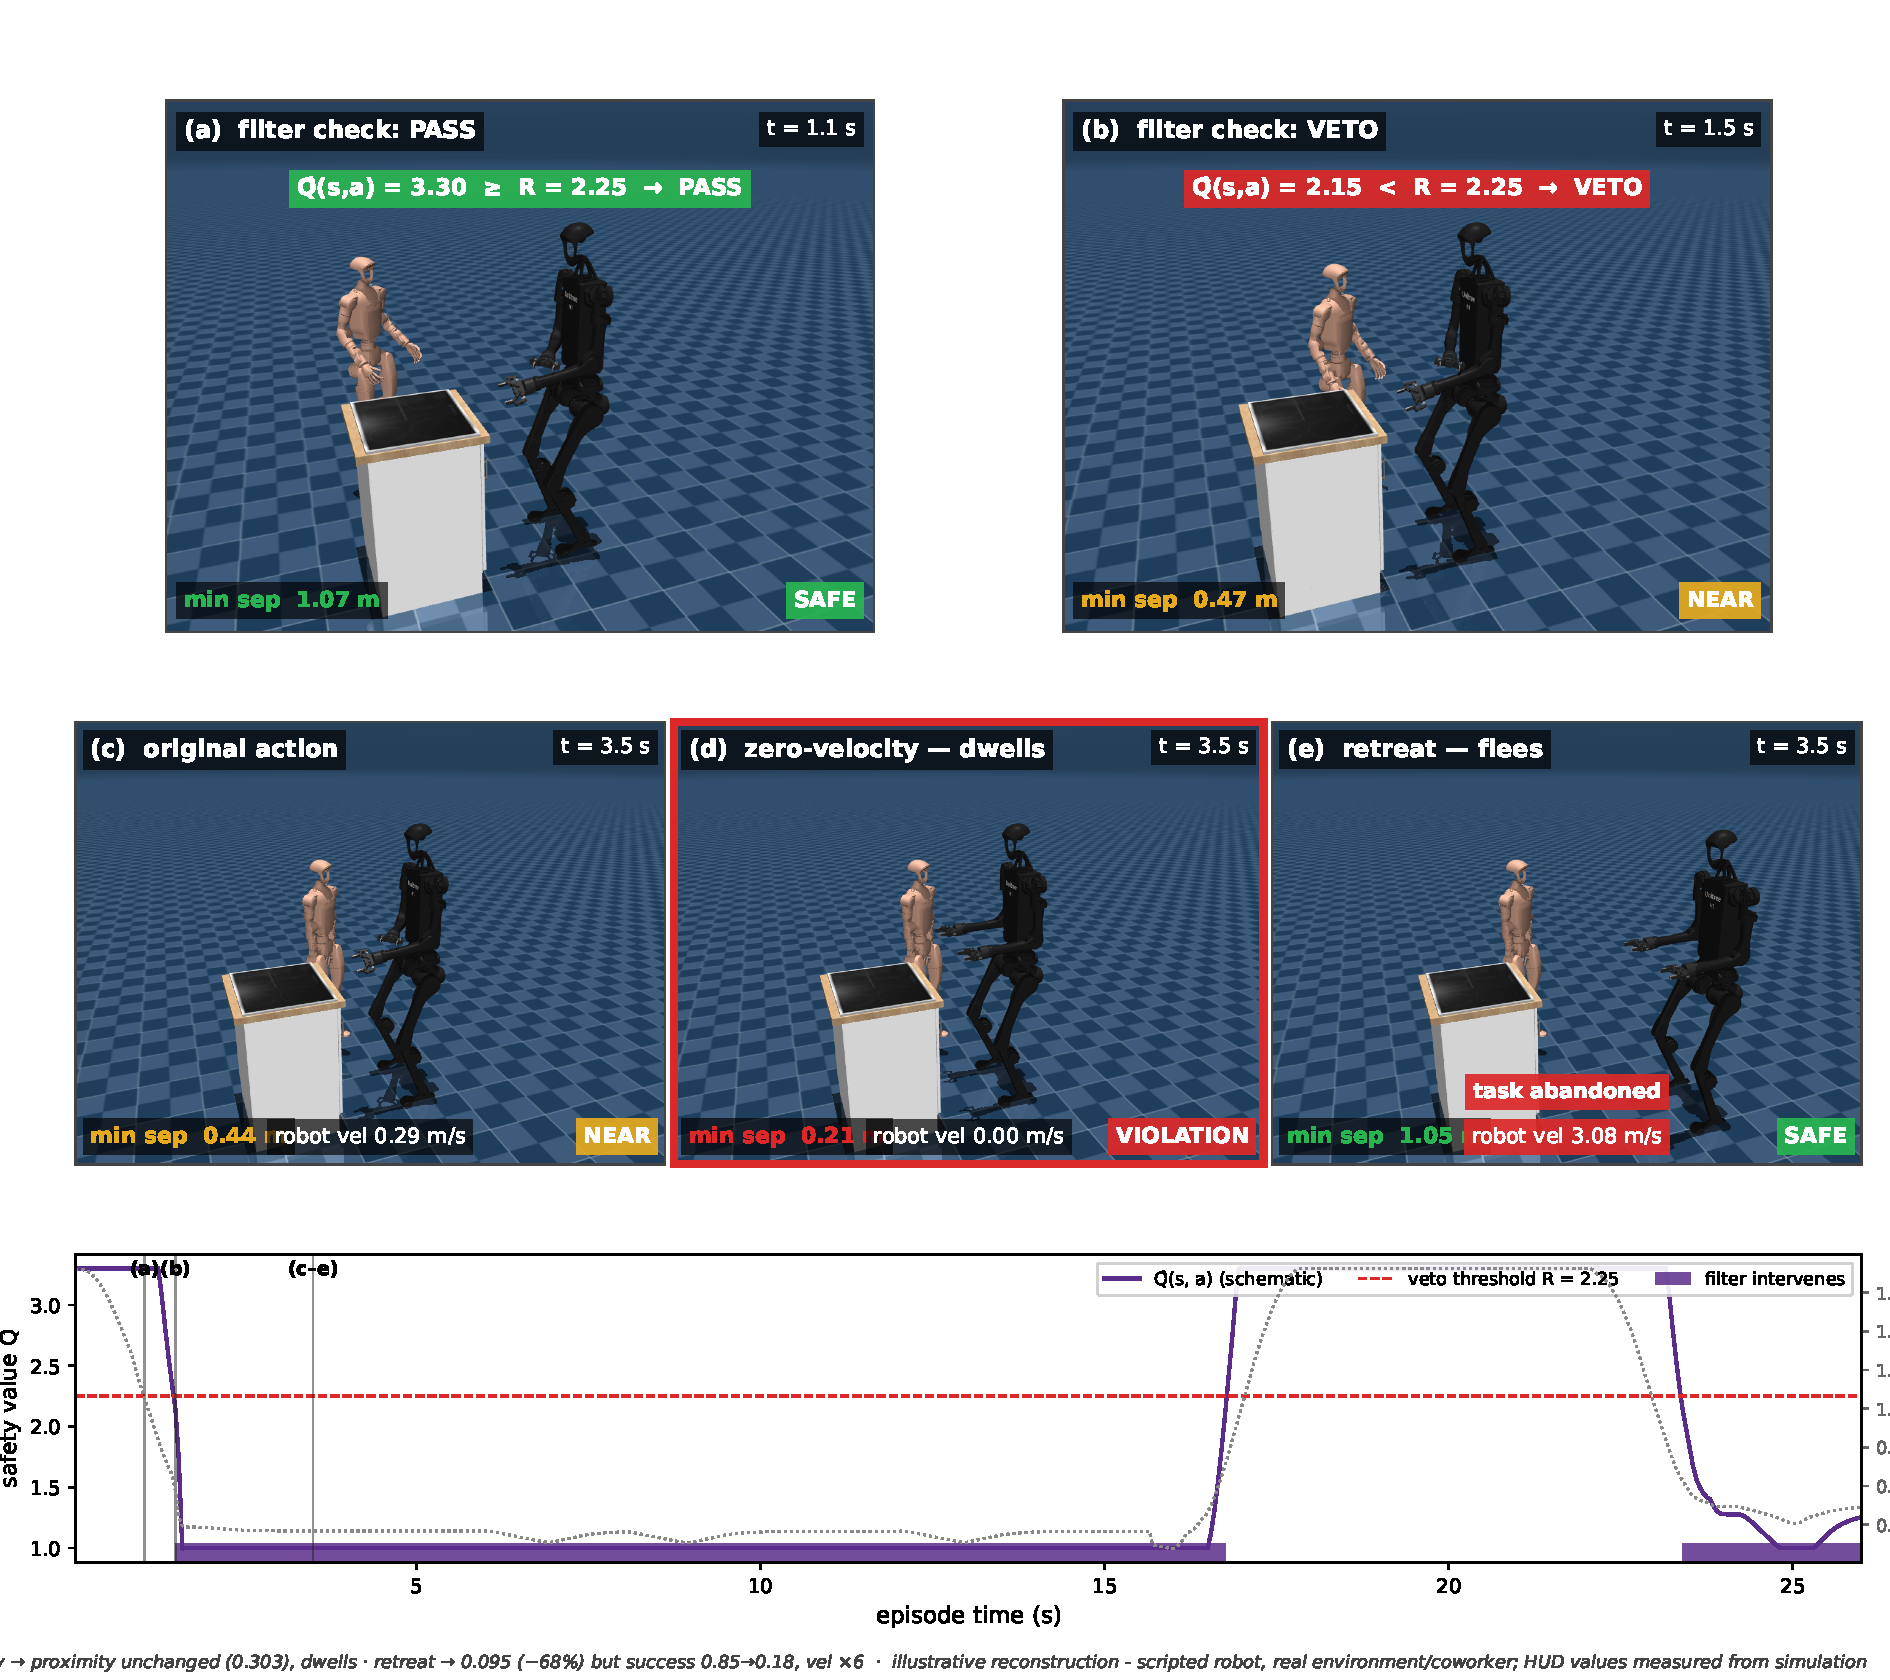
\includegraphics[width=\textwidth]{fig_svf_veto_anatomy}
\caption{Anatomy of the reactive SVF veto (illustrative reconstruction;
the $\hat{Q}$ trace is a schematic of the v3 critic's behaviour, and the
two fallbacks are the deployed implementations' semantics). Top: the
filter classifies a proposed action as safe (a) and, in the coworker's
reach window, unsafe (b). Middle: three continuations of the same veto
state, (c) the original action proceeds into the reach; (d) the
zero-velocity fallback freezes and \emph{dwells} in proximity as the
coworker keeps closing; (e) the retreat fallback flees, restoring
separation at the cost of the task and a velocity spike. Bottom:
$\hat{Q}$ against $R$ with intervention bands and the separation trace.
Benchmark aggregates (60 episodes each): zero-velocity leaves the
proximity-violation rate unchanged ($0.296 \to 0.303$) while dwelling;
retreat cuts it to $0.095$ ($-68\,\%$) but collapses success
$0.85 \to 0.18$ with $6\times$ mean velocity
(Table~\ref{tab:filter-taxonomy}).}
\label{fig:svf-veto-anatomy}
\end{figure}

\section{ISO-SSM Speed-Scaling}
\label{app:walk-speedscale}

Figure~\ref{fig:speedscale-mechanism} shows the velocity-axis
specialist (Section~\ref{sec:results:r2}): the graded speed-scaling
filter leaves the commanded \emph{direction} untouched and scales the
commanded per-step \emph{motion} by the closest separation,
$\mathrm{scale} = \mathrm{clip}\!\left((\mathrm{sep} - 0.15)/(0.40 -
0.15),\, 0,\, 1\right)$. It operates at full speed when the coworker is clear, a
graded slow-down as they approach, and a hold near contact.

\begin{figure}[htbp]
\centering
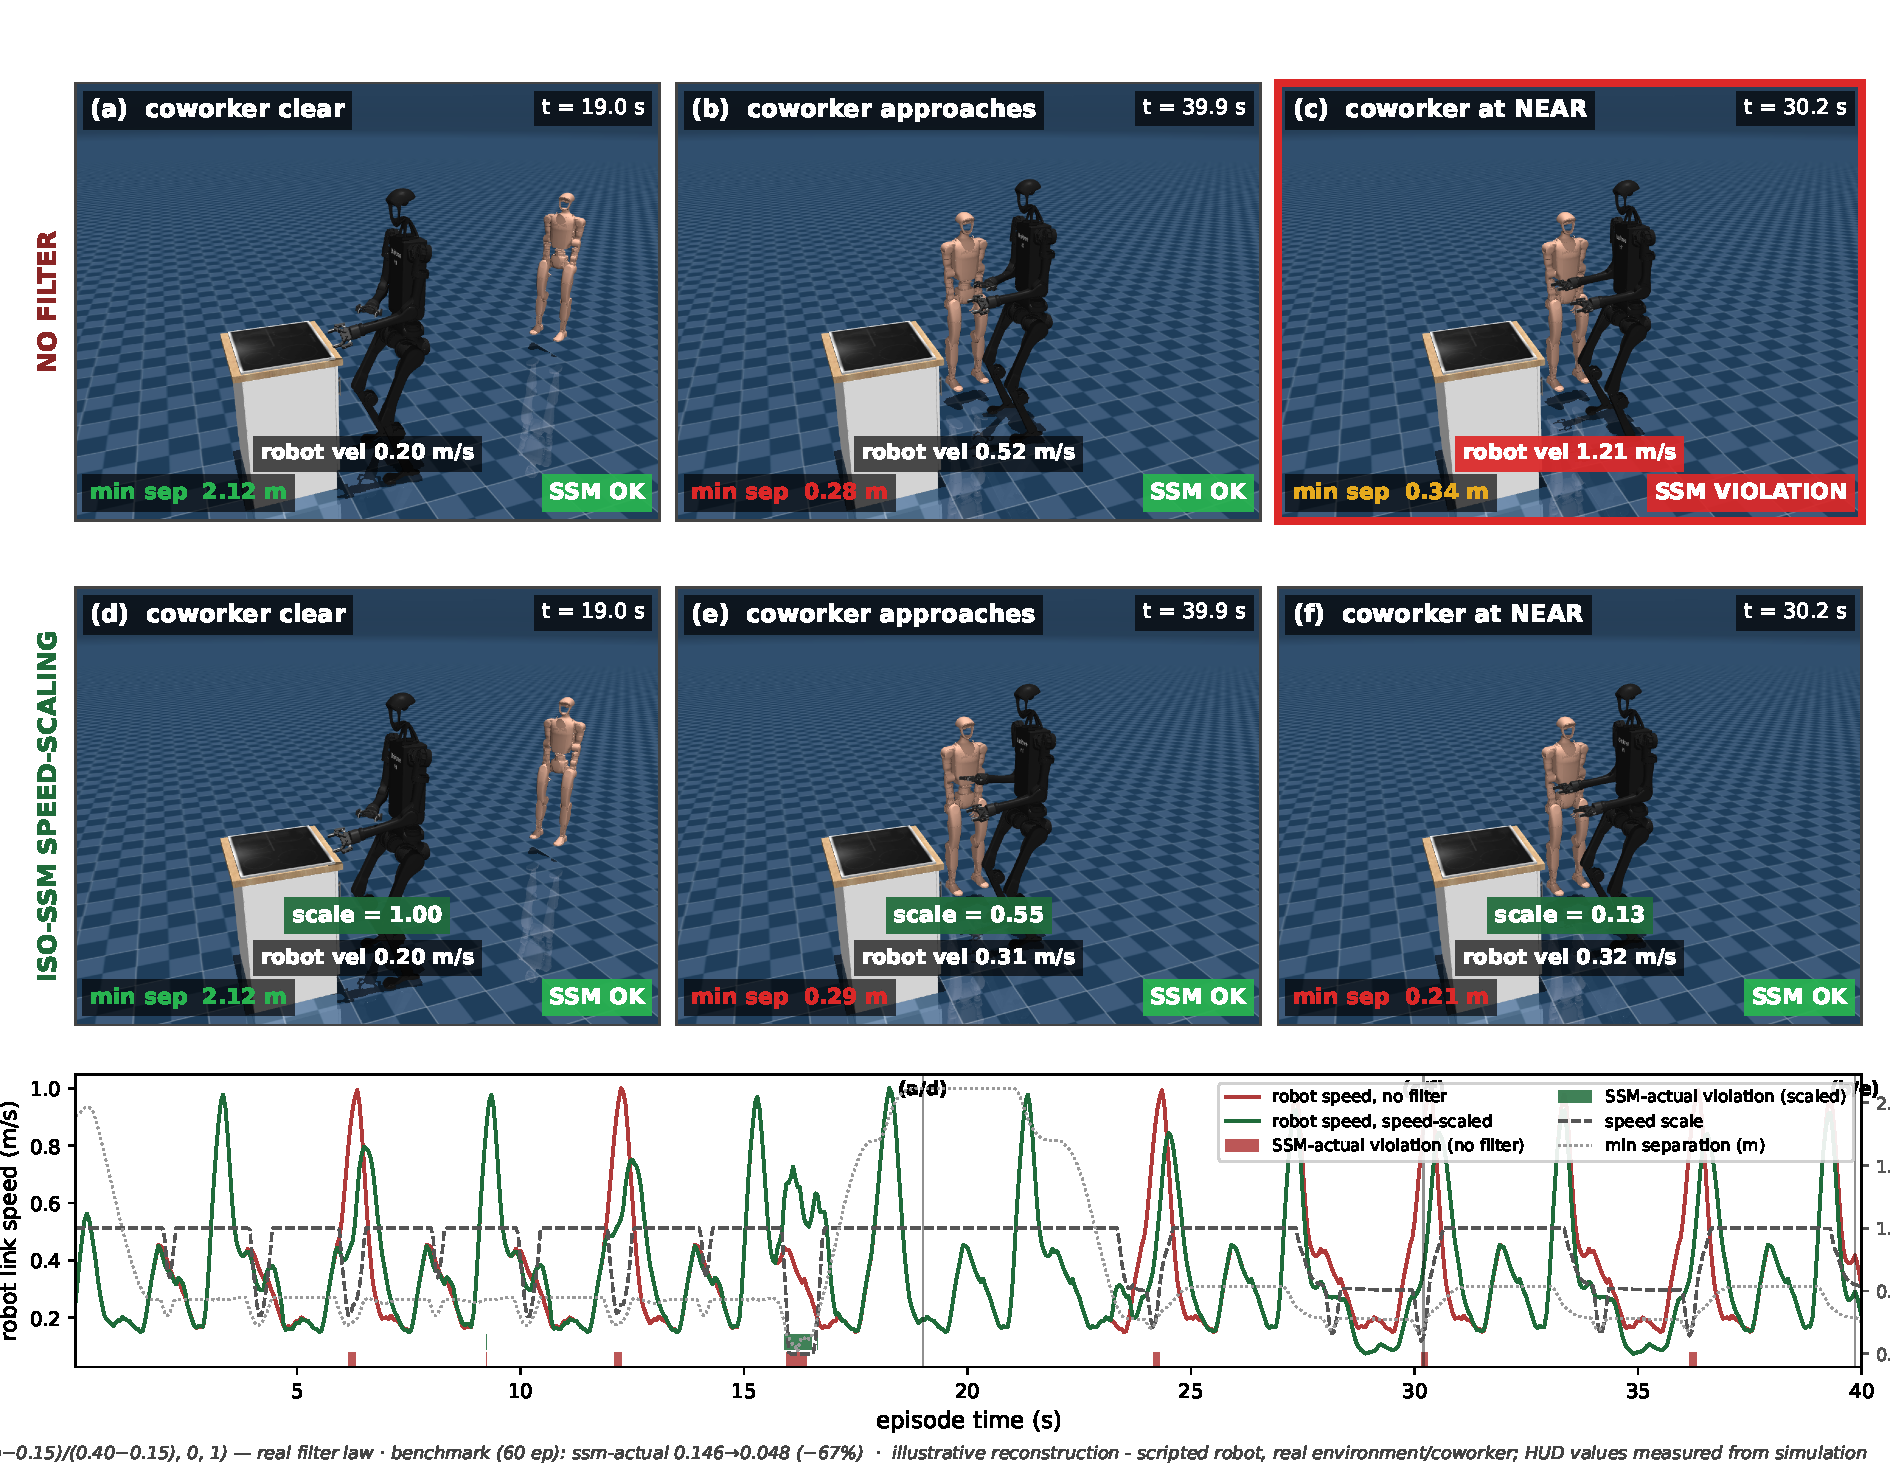
\includegraphics[width=\textwidth]{fig_speedscale_mechanism}
\caption{The ISO-SSM speed-scaling filter, frame by frame (illustrative
reconstruction; the scaling law shown is the deployed implementation's
formula acting on the same scripted task motion as the no-filter row,
which shuttles between work spots so it carries realistic velocity near
the coworker). \textbf{Borders and status chips on this figure mark the
\ssm{}-actual (velocity-adaptive) violation, the axis this filter
targets, not proximity, which it leaves unchanged by design.} Columns:
coworker clear (scale $= 1$, full speed), coworker approaching (graded
slow-down), coworker at \textsc{near}, where the unfiltered robot's
speed beside the coworker triggers an \ssm{} violation (top, red) while
the scaled robot moving at the same place and time does not (bottom,
green). Timeline: smoothed link speed for both runs with \ssm{}-actual
violation ribbons, the scale trace, and separation. In the benchmark,
\ssm{}-actual falls $0.146 \to 0.048$ ($-67\,\%$) at
$d_{\mathrm{slow}} = 0.40$\,m with geometric proximity essentially
unchanged ($0.296 \to 0.273$) (Figure~\ref{fig:velocity-axis}).}
\label{fig:speedscale-mechanism}
\end{figure}

\chapter{Use of Generative AI}
\label{app:genai}

Generative AI tools (Anthropic Claude, OpenAI ChatGPT) were used during
this project, and their use is declared here in full. Their role was
assistive and reviewable:
\begin{itemize}[topsep=2pt,itemsep=1pt]
\item \textbf{Literature search and triage.} AI tools helped shortlist
  candidate work in safe RL, CBF filtering, shielding, and human-aware
  robotics. Every retained citation was then checked manually against a
  primary source (arXiv, IEEE/ACM/PMLR/AAAI/NeurIPS/JMLR, ISO
  catalogue, or publisher page). 
\item \textbf{Code scaffolding.} AI tools drafted repetitive
  infrastructure such as data-loading helpers, wrapper boilerplate, and
  plotting scripts. Correctness-bearing code, including training loops,
  loss functions, cost signals, evaluation metrics, and aggregation
  logic, was reviewed, modified where necessary, and tested by the
  author before use.
\item \textbf{Experiment-log summarisation.} AI tools helped summarise
  large collections of CSVs, JSONL logs, and draft result notes into
  candidate tables or prose. Every numerical claim in the report was
  checked back to an artifact in \texttt{results/}, a documented script,
  or a saved figure-data note before inclusion.
\item \textbf{\LaTeX{} and prose.} AI tools assisted with \LaTeX{}
  formatting, restructuring, drafting, and proofreading. No AI-generated
  passage is included verbatim without author editing; the author chose
  the final framing, claims, section ordering, and wording.
\end{itemize}

The tools' limitations shaped the workflow. They sometimes overstated
ISO compliance or treated simulated \ssm{} improvements as real-world
certification, so all safety claims were edited back to the qualified
\ssm{}/proximity language of Section~\ref{sec:disc:pfl-bug}. All experimental design decisions, all
choices of what to run and measure, all quantitative results, and all
scientific claims are the author's responsibility.

\chapter{Ethical Considerations}
\label{app:ethics}

The project involves no human-subjects research and no personal data.
All human-motion data is from the publicly released AMASS
dataset~\cite{mahmood2019amass}, used under its research-only licence. No
real-robot deployment was conducted; the simulated humanoid--human
contact forces are not safety-validated for real-world use. The work
targets a safety standard (\iso{}) and aims to improve safety outcomes;
the principal ethical risk is over-claiming compliance and thereby
prompting under-validated deployment. This is mitigated by the qualified,
\ssm{}-only compliance claim of Section~\ref{sec:disc:pfl-bug}, by the
honest reporting of the safety--throughput trade rather than presenting
the safe configuration as free, and by the explicit recommendation in
Section~\ref{sec:disc:broader} that any real-world deployment require
independent validation and, for vulnerable users, stronger guarantees
than this work provides.

\chapter{Sustainability}
\label{app:sustainability}

Total compute was roughly $450$--$500$\,GPU-hours on NVIDIA A100
(40\,GB) GPUs (Section~\ref{sec:setup:compute}): $\approx$220\,h for
the persistent-co-location arc, reconstructed from run logs, plus
$\approx$230--280\,h for the intermittent-co-location arc and the
WCSAC external baseline, of which the six 150k-frame from-scratch
WCSAC runs dominate and are estimated rather than log-reconstructed.
At an assumed mean board power of $0.3$\,kW and a data-centre
power-usage effectiveness of $1.4$, the midpoint ($\approx$475\,h) is
approximately $200$\,kWh; at the 2024 UK grid carbon intensity of
$0.21$\,kg\,CO\textsubscript{2}e/kWh, approximately
$40$\,kg\,CO\textsubscript{2}e. Several practices kept this figure low: resumable
training with checkpoint reuse; CPU smoke gates before every multi-hour
training launch; deliberate seed-count selection (3--5) balancing
statistical confidence against compute; warm-starting the constrained
policy from the Phase~1 base-policy snapshot rather than retraining the
task from scratch (Section~\ref{sec:method:lagrangian:warmstart}); and
snapshot-only Phase~2 dataset collection, which avoids a separate, slow
random-rollout pass. The dominant cost is policy training, not
evaluation; the snapshot harness makes re-evaluation effectively free
relative to a retrain.

\chapter{Code and Data Availability}
\label{app:data}

The code, including the \sbigym{} benchmark, all runtime-filter
implementations, the training entry points, and the
snapshot-evaluation harness
(\texttt{scripts/benchmark\_policy.py},
Section~\ref{sec:bench:harness}), is available at
\url{https://github.com/ayushpatel4/safety-bigym-2}. Pre-trained weights for
the headline fixed-$\lambda$ policy (the three selected checkpoints
listed in Appendix~\ref{app:repro}), the \texttt{saucepan\_to\_hob}
SVF critic and the shared \texttt{dishwasher\_close}/\texttt{drawers\_open\_all}
SVF critic together with their dataset shards
(37{,}883 and 52{,}794 transitions respectively), the WCSAC
checkpoints, and the per-cell benchmark CSVs behind every results
table (including the gated, ablation, and boundary sweeps) are
archived on the project's experiment workstation and are available
from the author on request while a hosted release is prepared. Every
quantitative table in this report is regenerable from those
snapshots with the harness, without any retraining. 

% =============================================================================
\end{document}
% =============================================================================